\documentclass{book}
\usepackage[utf8]{inputenc}
\usepackage[greek.polutoniko,french]{babel}
\usepackage{ebgaramond-maths}
\usepackage{arabtex}
\usepackage[normalem]{ulem}
\usepackage{graphicx}
\usepackage[colorlinks]{hyperref}
\usepackage{glossaries}

\title{Lettres d'Auguste Mariette}
\author{Thomas Lebée}
\date{Février 2020}

\hypersetup{
    colorlinks=true,
    linkcolor=blue,
    filecolor=blue,      
    urlcolor=blue,
}
\graphicspath{ {./images/} }

\newglossary[]{place}{}{}{Lieux}{}
\newglossary[]{contemp}{}{}{Contemporains de Mariette}{}
\newglossary[]{hist}{}{}{Personnages historiques}{}
\newglossary[]{myth}{}{}{Figures mythiques et religieuses}{}
\newglossary[]{abbr}{}{}{Abréviations}{}
\newglossary[]{boat}{}{}{Bateaux}{}
\newglossary[]{term}{}{}{Glossaire}{}
\newglossary[]{stela}{}{}{Stèles}{}
\newglossary[]{statue}{}{}{Statues}{}
\newglossary[]{misc}{}{}{Divers}{}
\newglossary[]{org}{}{}{Institutions}{}
\newglossary[]{bibl}{}{}{Publications}{}

\makenoidxglossaries

\newglossaryentry{CoEg_pers_00000001}{name={Mariette [Pacha], Auguste},type={contemp},text=*,description={Égyptologue (1821-1881) [\href{https://www.wikidata.org/wiki/Q311850}{Wikidata}]}}
\newglossaryentry{CoEg_pers_imn}{name={À identifier},sort={aaa},type={contemp},text=*,description={Personne non encore identifiée}}
\newglossaryentry{CoEg_pers_00000002}{name={Nieuwerkerke (de), Émilien},type={contemp},text=*,description={Artiste et homme d'État (1811-1892).  Il fut successivement directeur général des musées, intendant des beaux-arts et surintendant des musées impériaux [\href{https://www.wikidata.org/wiki/Q1232403}{Wikidata}]}}
\newglossaryentry{CoEg_pers_00000003}{name={Esquirou de Parieu, Félix},type={contemp},text=*,description={Homme d'État (1815-1893). Ministre de l'Instruction publique en 1850 [\href{https://www.wikidata.org/wiki/Q535804}{Wikidata}]}}
\newglossaryentry{CoEg_pers_00000004}{name={Baroche, Jules},type={contemp},text=*,description={Homme d'État (1802-1870). Ministre de l'Intérieur en 1850 [\href{https://www.wikidata.org/wiki/Q3385651}{Wikidata}]}}
\newglossaryentry{CoEg_pers_00000005}{name={Millon (épouse Mariette), Éléonore},type={contemp},text=*,description={Épouse de Mariette (1827-1865)}}
\newglossaryentry{CoEg_pers_00000006}{name={Mariette, Marguerite Louise},type={contemp},text=*,description={Fille de Mariette (1846-1861)}}
\newglossaryentry{CoEg_pers_00000007}{name={Mariette, Joséphine Cornélie},type={contemp},text=*,description={Fille de Mariette (1847-1873)}}
\newglossaryentry{CoEg_pers_00000008}{name={Mariette, Sophie Éléonore},type={contemp},text=*,description={Fille de Mariette (1849-1885)}}
\newglossaryentry{CoEg_pers_00000009}{name={Néphéritès Ier},type={hist},text=*,description={Roi égyptien [\href{https://www.wikidata.org/wiki/Q450994}{Wikidata}]}}
\newglossaryentry{CoEg_pers_00000010}{name={Amyrtée},type={hist},text=*,description={Roi égyptien [\href{https://www.wikidata.org/wiki/Q318000}{Wikidata}]}}
\newglossaryentry{CoEg_pers_00000011}{name={Apis},type={myth},text=*,description={Taureau sacré de Ptah à Memphis [\href{https://www.wikidata.org/wiki/Q208150}{Wikidata}]}}
\newglossaryentry{CoEg_pers_00000012}{name={Seth},type={myth},text=*,description={Dieu égyptienMariette utilise la désignation grecque \og ~Typhon~\fg [\href{https://www.wikidata.org/wiki/Q131795}{Wikidata}]}}
\newglossaryentry{CoEg_pers_00000013}{name={Nectanébo},type={hist},text=*,description={Roi égyptien}}
\newglossaryentry{CoEg_pers_00000014}{name={Lafuente},type={contemp},text=*,description={}}
\newglossaryentry{CoEg_pers_00000015}{name={D'Anastasi, Giovanni},type={contemp},text=*,description={Marchand et antiquaire (1765-1860) [\href{https://www.wikidata.org/wiki/Q5563656}{Wikidata}]}}
\newglossaryentry{CoEg_pers_00000016}{name={Abbas Pacha},type={contemp},text=*,description={Vice-roi d'Égypte (1813-1854) [\href{https://www.wikidata.org/wiki/Q305882}{Wikidata}]}}
\newglossaryentry{CoEg_pers_00000017}{name={Méhémet Ali},type={contemp},text=*,description={Vice-roi d'Égypte (1769-1849) [\href{https://www.wikidata.org/wiki/Q182781}{Wikidata}]}}
\newglossaryentry{CoEg_pers_00000018}{name={Murray, Charles},type={contemp},text=*,description={Diplomate (1806-1895). Consul britannique en Égypte de 1846 à 1853 [\href{https://www.wikidata.org/wiki/Q1063616}{Wikidata}]}}
\newglossaryentry{CoEg_pers_00000019}{name={Linant de Bellefonds [Pacha], Louis Maurice Adolphe},type={contemp},text=*,description={Ingénieur (1798-1883) [\href{https://www.wikidata.org/wiki/Q960740}{Wikidata}]}}
\newglossaryentry{CoEg_pers_00000020}{name={Lambert [Bey], Charles Joseph},type={contemp},text=*,description={Ingénieur (1804-1864) [\href{https://www.wikidata.org/wiki/Q18744680}{Wikidata}]}}
\newglossaryentry{CoEg_pers_00000021}{name={Clot [Bey], Antoine},type={contemp},text=*,description={Médecin[\href{https://www.wikidata.org/wiki/Q2372786}{Wikidata}]}}
\newglossaryentry{CoEg_pers_00000022}{name={Varin [Bey], Noël},type={contemp},text=*,description={Militaire (1784-1863)}}
\newglossaryentry{CoEg_pers_00000023}{name={Walker [Bey]},type={contemp},text=*,description={Boulanger britannique d'Abbas Pacha}}
\newglossaryentry{CoEg_pers_00000024}{name={Le Moyne, A.},type={contemp},text=*,description={DiplomateConsul général et agent de France en Égypte ; remplacé par Sabatier à l'été 1852}}
\newglossaryentry{CoEg_pers_00000025}{name={Benedetti, Vincent},type={contemp},text=*,description={Diplomate (1817-1900). Gendre d'Anastasi\gls{CoEg_pers_00000015} [\href{https://www.wikidata.org/wiki/Q1350848}{Wikidata}]}}
\newglossaryentry{CoEg_pers_00000026}{name={Ramsès II},type={hist},text=*,description={Roi égyptien [\href{https://www.wikidata.org/wiki/Q1523}{Wikidata}]}}
\newglossaryentry{CoEg_pers_00000027}{name={Batissier, Louis},type={contemp},text=*,description={ (1813-1882). Vice-consul à Suez entre 1848 et 1861}}
\newglossaryentry{CoEg_pers_00000028}{name={Safar-Pacha},type={contemp},text=*,description={Moudir\gls{CoEg_term_00000004} de Giza\gls{CoEg_place_00000007}}}
\newglossaryentry{CoEg_pers_00000029}{name={Stéphan Bey},type={contemp},text=*,description={ministre égyptien des Affaires étrangères}}
\newglossaryentry{CoEg_pers_00000030}{name={Cambyse},type={hist},text=*,description={Roi perse [\href{https://www.wikidata.org/wiki/Q182483}{Wikidata}]}}
\newglossaryentry{CoEg_pers_00000031}{name={Diodore de Sicile},type={hist},text=*,description={Historien grec [\href{https://www.wikidata.org/wiki/Q171241}{Wikidata}]}}
\newglossaryentry{CoEg_pers_00000032}{name={Rougé (de), Emmanuel},type={contemp},text=*,description={Égyptologue (1811-1872) [\href{https://www.wikidata.org/wiki/Q2087467}{Wikidata}]}}
\newglossaryentry{CoEg_pers_00000033}{name={Longpérier (de), Adrien},type={contemp},text=*,description={Archéologue (1816-1882) [\href{https://www.wikidata.org/wiki/Q127218}{Wikidata}]}}
\newglossaryentry{CoEg_pers_00000034}{name={Viel-Castel (de), Horace},type={contemp},text=*,description={Historien d'art (1802-1864) [\href{https://www.wikidata.org/wiki/Q3140481}{Wikidata}]}}
\newglossaryentry{CoEg_pers_00000035}{name={Villot, Frédéric},type={contemp},text=*,description={Graveur et historien d'art (1809-1875) [\href{https://www.wikidata.org/wiki/Q3090265}{Wikidata}]}}
\newglossaryentry{CoEg_pers_00000036}{name={Dieu},type={myth},text=*,description={[\href{https://www.wikidata.org/wiki/Q190}{Wikidata}]}}
\newglossaryentry{CoEg_pers_00000037}{name={Victor Fialin de Persigny},type={contemp},text=*,description={ (1808-1872). Ministre de l'Intérieur et des Beaux-Arts [\href{https://www.wikidata.org/wiki/Q3174556}{Wikidata}]}}
\newglossaryentry{CoEg_pers_00000038}{name={Boujon},type={contemp},text=*,description={}}
\newglossaryentry{CoEg_pers_00000039}{name={Verrier},type={contemp},text=*,description={}}
\newglossaryentry{CoEg_pers_00000040}{name={Sabatier},type={contemp},text=*,description={Diplomate. Consul général de France en Égypte ; succède à Le Moyne au cours de l'été 1852}}
\newglossaryentry{CoEg_pers_00000041}{name={Drouyn de Lhuys, Édouard},type={contemp},text=*,description={ (1805-1881). Ministre français des Affaires étrangères [\href{https://www.wikidata.org/wiki/Q274294}{Wikidata}]}}
\newglossaryentry{CoEg_pers_00000042}{name={Osiris},type={myth},text=*,description={Dieu égyptien [\href{https://www.wikidata.org/wiki/Q46491}{Wikidata}]}}
\newglossaryentry{CoEg_pers_00000043}{name={An/ugn/uiot ?},type={contemp},text=*,description={}}
\newglossaryentry{CoEg_pers_00000044}{name={Sauzay/Lanzay (de) ?},type={contemp},text=*,description={}}
\newglossaryentry{CoEg_pers_00000045}{name={N.},type={contemp},text=*,description={second drogman du consulat général à l'été 1852}}
\newglossaryentry{CoEg_pers_00000046}{name={Pastré, Eugène},type={contemp},text=*,description={ (1806-1868) [\href{https://www.wikidata.org/wiki/Q5408576}{Wikidata}]}}
\newglossaryentry{CoEg_pers_00000047}{name={Ptah},type={myth},text=*,description={Dieu égyptien. Patron de Memphis [\href{https://www.wikidata.org/wiki/Q146321}{Wikidata}]}}
\newglossaryentry{CoEg_pers_00000048}{name={Hékékyan Bey},type={contemp},text=*,description={}}
\newglossaryentry{CoEg_pers_00000049}{name={Fleury Hérard},type={contemp},text=*,description={BanquierBanquier ordinaire à Paris du corps diplomatique}}
\newglossaryentry{CoEg_pers_00000050}{name={Aïdi},type={contemp},text=*,description={}}
\newglossaryentry{CoEg_pers_00000051}{name={Brunet de Presle, Wladimir},type={contemp},text=*,description={ (1809-1875) [\href{https://www.wikidata.org/wiki/Q4097433}{Wikidata}]}}
\newglossaryentry{CoEg_pers_00000052}{name={Le Moyne, Auguste},type={contemp},text=*,description={Fils de Le Moyne\gls{CoEg_pers_00000024}}}
\newglossaryentry{CoEg_pers_00000053}{name={Le Moyne, madame},type={contemp},text=*,description={Épouse de Le Moyne\gls{CoEg_pers_00000024}}}
\newglossaryentry{CoEg_pers_00000054}{name={Brey de Prusser},type={contemp},text=*,description={}}
\newglossaryentry{CoEg_pers_00000055}{name={Artaxerxes III},type={hist},text=*,description={Roi perse [\href{https://www.wikidata.org/wiki/Q192867}{Wikidata}]}}
\newglossaryentry{CoEg_pers_00000057}{name={Darius},type={hist},text=*,description={Roi perse [\href{https://www.wikidata.org/wiki/Q44387}{Wikidata}]}}
\newglossaryentry{CoEg_pers_00000058}{name={Amasis},type={hist},text=*,description={Roi égyptien [\href{https://www.wikidata.org/wiki/Q312045}{Wikidata}]}}
\newglossaryentry{CoEg_pers_00000059}{name={Soliman Pacha},type={contemp},text=*,description={Militaire français, né Joseph Seve, passé au service de l'Égypte (1788-1860) [\href{https://www.wikidata.org/wiki/Q745216}{Wikidata}]}}
\newglossaryentry{CoEg_pers_00000060}{name={Sérapis},type={myth},text=*,description={Dieu égyptien [\href{https://www.wikidata.org/wiki/Q214554}{Wikidata}]}}
\newglossaryentry{CoEg_pers_00000061}{name={Lepsius, Karl Richard},type={contemp},text=*,description={Égyptologue (1810-1884) [\href{https://www.wikidata.org/wiki/Q77231}{Wikidata}]}}
\newglossaryentry{CoEg_pers_00000062}{name={Fouad Effendi},type={contemp},text=*,description={}}
\newglossaryentry{CoEg_pers_00000063}{name={Apriès},type={hist},text=*,description={Roi égyptien [\href{https://www.wikidata.org/wiki/Q349291}{Wikidata}]}}
\newglossaryentry{CoEg_pers_00000064}{name={Chechonq III},type={hist},text=*,description={Roi égyptien [\href{https://www.wikidata.org/wiki/Q878396}{Wikidata}]}}
\newglossaryentry{CoEg_pers_00000066}{name={Neshor},type={hist},text=*,description={}}
\newglossaryentry{CoEg_pers_00000067}{name={Delaporte, Pacifique-Henri},type={contemp},text=*,description={ (1816-1877). Consul français au Caire  [\href{https://www.wikidata.org/wiki/Q47461240}{Wikidata}]}}
\newglossaryentry{CoEg_pers_00000068}{name={Anubis},type={myth},text=*,description={Dieu égyptien [\href{https://www.wikidata.org/wiki/Q47534}{Wikidata}]}}
\newglossaryentry{CoEg_pers_00000069}{name={Antef},type={hist},text=*,description={}}
\newglossaryentry{CoEg_pers_00000070}{name={Bonnefoy},type={contemp},text=*,description={}}
\newglossaryentry{CoEg_pers_00000071}{name={Napoléon III},type={contemp},text=*,description={Empereur des Français (1808-1873) [\href{https://www.wikidata.org/wiki/Q7721}{Wikidata}]}}
\newglossaryentry{CoEg_pers_00000072}{name={Allah},type={myth},text=*,description={[\href{https://www.wikidata.org/wiki/Q234801}{Wikidata}]}}
\newglossaryentry{CoEg_pers_00000073}{name={Albatros (L')},type={boat},text=*,description={}}
\newglossaryentry{CoEg_pers_00000074}{name={Bonaparte, Napoléon-Jérôme},type={contemp},text=*,description={Prince français (1822-1891) [\href{https://www.wikidata.org/wiki/Q434077}{Wikidata}]}}
\newglossaryentry{CoEg_pers_00000075}{name={ Fould, Achille},type={contemp},text=*,description={Homme d'État (1800-1867) [\href{https://www.wikidata.org/wiki/Q340215}{Wikidata}]}}
\newglossaryentry{CoEg_pers_00000076}{name={Eugénie (impératrice)},type={contemp},text=*,description={Impératrice, épouse de Napoléon III\gls{CoEg_pers_00000071} (1826-1920) [\href{https://www.wikidata.org/wiki/Q157130}{Wikidata}]}}
\newglossaryentry{CoEg_pers_00000077}{name={Louis-Philippe I\textsuperscript{er}},type={contemp},text=*,description={Roi des Français (1773-1850) [\href{https://www.wikidata.org/wiki/Q7771}{Wikidata}]}}
\newglossaryentry{CoEg_pers_00000078}{name={Billaut, Adolphe},type={contemp},text=*,description={Homme d'État (1805-1863). Ministre de l'Intérieur [\href{https://www.wikidata.org/wiki/Q505189}{Wikidata}]}}
\newglossaryentry{CoEg_pers_00000079}{name={Morny (de), Charles},type={contemp},text=*,description={Homme d'État (1811-1865) [\href{https://www.wikidata.org/wiki/Q965335}{Wikidata}]}}
\newglossaryentry{CoEg_pers_00000080}{name={Saïd Pacha},type={contemp},text=*,description={Vice-roi d'Égypte (1822-1863) [\href{https://www.wikidata.org/wiki/Q366744}{Wikidata}]}}
\newglossaryentry{CoEg_pers_00000081}{name={Ferri-Pisani, Camille},type={contemp},text=*,description={Officier militaire. (1819-1893). Aide-de-camp du prince Napoléon\gls{CoEg_pers_00000074} [\href{https://www.wikidata.org/wiki/Q23054685}{Wikidata}]}}
\newglossaryentry{CoEg_pers_00000082}{name={Devéria, Théodule},type={contemp},text=*,description={Égyptologue (1831-1871) [\href{https://www.wikidata.org/wiki/Q406953}{Wikidata}]}}
\newglossaryentry{CoEg_pers_00000083}{name={Mariette, Émilie Marie},type={contemp},text=*,description={Fille de Mariette (1855-1871)}}
\newglossaryentry{CoEg_pers_00000084}{name={Mariette, Alphonse Paulin},type={contemp},text=*,description={Fils de Mariette (1856-1879)}}

\newglossaryentry{CoEg_org_imn}{name={À identifier},sort={aaa},type={org},text=*,description={Institution non encore identifiée}}
\newglossaryentry{CoEg_org_00000011}{name={Beaux-Arts (administration)},type={org},text=*,description={[note : préciser le substantif adapté en 1852 et par la suite]}}
\newglossaryentry{CoEg_org_00000024}{name={Archives nationales},type={org},text=*,description={ [\href{https://www.wikidata.org/wiki/Q182542}{Wikidata}]}}
\newglossaryentry{CoEg_org_00000013}{name={Armée égyptienne},type={org},text=*,description={ [\href{https://www.wikidata.org/wiki/Q1075553}{Wikidata}]}}
\newglossaryentry{CoEg_org_00000005}{name={British Museum},type={org},text=*,description={ [\href{https://www.wikidata.org/wiki/Q6373}{Wikidata}]}}
\newglossaryentry{CoEg_org_00000023}{name={Collège de France},type={org},text=*,description={ [\href{https://www.wikidata.org/wiki/Q202660}{Wikidata}]}}
\newglossaryentry{CoEg_org_00000006}{name={Consulat général de France à Alexandrie},type={org},text=*,description={L'Égypte étant théoriquement une province de l'Empire ottoman, les puissances étrangères ne pouvaient y entretenir d'ambassade ; les intérêts français étaient représentés par l'\og agence diplomatique et consulat général\fg, à Alexandrie\gls{CoEg_place_00000006}. Mariette\gls{CoEg_pers_00000001} connut les consuls généraux successifs Le Moyne\gls{CoEg_pers_00000024} et Sabatier\gls{CoEg_pers_00000040}}}
\newglossaryentry{CoEg_org_00000020}{name={Louvre (musée), département égyptien},type={org},text=*,description={Division du musée du Louvre\gls{CoEg_org_00000002}.}}
\newglossaryentry{CoEg_org_00000014}{name={Gouvernement britannique},type={org},text=*,description={ [\href{https://www.wikidata.org/wiki/Q6063}{Wikidata}]}}
\newglossaryentry{CoEg_org_00000008}{name={Gouvernement égyptien},type={org},text=*,description={ [\href{https://www.wikidata.org/wiki/Q33121876}{Wikidata}]}}
\newglossaryentry{CoEg_org_00000012}{name={Gouvernement français},type={org},text=*,description={Désigne aussi plus généralement l'État [\href{https://www.wikidata.org/wiki/Q1450662}{Wikidata}]}}
\newglossaryentry{CoEg_org_00000004}{name={Institut de France},type={org},text=*,description={ [\href{https://www.wikidata.org/wiki/Q377066}{Wikidata}]}}
\newglossaryentry{CoEg_org_00000010}{name={État et maison de l'empereur (ministère)},type={org},text=*,description={}}
\newglossaryentry{CoEg_org_00000017}{name={Instruction publique (ministère égyptien)},type={org},text=*,description={}}
\newglossaryentry{CoEg_org_00000016}{name={Travaux publics (ministère égyptien)},type={org},text=*,description={}}
\newglossaryentry{CoEg_org_00000009}{name={Intérieur (ministère français)},type={org},text=*,description={ [\href{https://www.wikidata.org/wiki/Q1518496}{Wikidata}]}}
\newglossaryentry{CoEg_org_00000019}{name={Marine (Ministère français)},type={org},text=*,description={}}
\newglossaryentry{CoEg_org_00000007}{name={Affaires étrangères (ministère français)},type={org},text=*,description={ [\href{https://www.wikidata.org/wiki/Q789848}{Wikidata}]}}
\newglossaryentry{CoEg_org_00000022}{name={Boulaq (musée)},type={org},text=*,description={ [\href{https://www.wikidata.org/wiki/Q2399429}{Wikidata}]}}
\newglossaryentry{CoEg_org_00000021}{name={Turin (musée)},type={org},text=*,description={ [\href{https://www.wikidata.org/wiki/Q19877}{Wikidata}]}}
\newglossaryentry{CoEg_org_00000002}{name={Louvre (musée)},type={org},text=*,description={ [\href{https://www.wikidata.org/wiki/Q19675}{Wikidata}]}}
\newglossaryentry{CoEg_org_00000003}{name={Vatican (musée)},type={org},text=*,description={ [\href{https://www.wikidata.org/wiki/Q526381}{Wikidata}]}}
\newglossaryentry{CoEg_org_00000018}{name={Louvre (musée), musée ethnographique},type={org},text=*,description={Division du musée du Louvre\gls{CoEg_org_00000002}.}}
\newglossaryentry{CoEg_org_00000001}{name={Musée nationaux/impériaux (direction)},type={org},text=*,description={}}
\newglossaryentry{CoEg_org_00000015}{name={Société géologique de Londres},type={org},text=*,description={ [\href{https://www.wikidata.org/wiki/Q1230936}{Wikidata}]}}

\newglossaryentry{CoEg_place_imn}{name={À identifier},sort={aaa},type={place},text=*,description={Lieu non encore identifié}}
\newglossaryentry{CoEg_place_00000008}{name={Abousyr},type={place},text=*,description={ [\href{https://www.wikidata.org/wiki/Q336098}{Wikidata}]}}
\newglossaryentry{CoEg_place_00000026}{name={Abydos},type={place},text=*,description={ [\href{https://www.wikidata.org/wiki/Q192268}{Wikidata}]}}
\newglossaryentry{CoEg_place_00000006}{name={Alexandrie},type={place},text=*,description={ [\href{https://www.wikidata.org/wiki/Q87}{Wikidata}]}}
\newglossaryentry{CoEg_place_00000022}{name={Algérie},type={place},text=*,description={ [\href{https://www.wikidata.org/wiki/Q262}{Wikidata}]}}
\newglossaryentry{CoEg_place_00000033}{name={Assiout},type={place},text=*,description={ [\href{https://www.wikidata.org/wiki/Q29962}{Wikidata}]}}
\newglossaryentry{CoEg_place_00000030}{name={Atfih},type={place},text=*,description={Poste de douane entre Boulaq\gls{CoEg_place_00000029} et Alexandrie\gls{CoEg_place_00000006} (Al-'Atf, près de Mahmudiyya, sur le canal de Rosette ?)}}
\newglossaryentry{CoEg_place_00000031}{name={Badrashyn},type={place},text=*,description={Village sur le Nil\gls{CoEg_place_00000021}, au voisinnage immédiat de Saqqara\gls{CoEg_place_00000001} et de Mit Rahineh\gls{CoEg_place_00000025}.Mariette\gls{CoEg_pers_00000001} écrit \og ~Bédréchyn~\fg.}}
\newglossaryentry{CoEg_place_00000029}{name={Boulaq},type={place},text=*,description={ [\href{https://www.wikidata.org/wiki/Q1003523}{Wikidata}]}}
\newglossaryentry{CoEg_place_00000023}{name={Citadelle du Caire},type={place},text=*,description={ [\href{https://www.wikidata.org/wiki/Q1988240}{Wikidata}]}}
\newglossaryentry{CoEg_place_00000028}{name={Dachour},type={place},text=*,description={ [\href{https://www.wikidata.org/wiki/Q685414}{Wikidata}]}}
\newglossaryentry{CoEg_place_00000003}{name={Égypte},type={place},text=*,description={ [\href{https://www.wikidata.org/wiki/Q79}{Wikidata}]}}
\newglossaryentry{CoEg_place_00000013}{name={Europe},type={place},text=*,description={ [\href{https://www.wikidata.org/wiki/Q46}{Wikidata}]}}
\newglossaryentry{CoEg_place_00000016}{name={France},type={place},text=*,description={ [\href{https://www.wikidata.org/wiki/Q142}{Wikidata}]}}
\newglossaryentry{CoEg_place_00000007}{name={Giza},type={place},text=*,description={ [\href{https://www.wikidata.org/wiki/Q81788}{Wikidata}]}}
\newglossaryentry{CoEg_place_00000020}{name={Haute-Egypte},type={place},text=*,description={ [\href{https://www.wikidata.org/wiki/Q203751}{Wikidata}]}}
\newglossaryentry{CoEg_place_00000024}{name={Héliopolis},type={place},text=*,description={ [\href{https://www.wikidata.org/wiki/Q191687}{Wikidata}]}}
\newglossaryentry{CoEg_place_00000010}{name={Le Caire},type={place},text=*,description={ [\href{https://www.wikidata.org/wiki/Q85}{Wikidata}]}}
\newglossaryentry{CoEg_place_00000027}{name={Le Havre},type={place},text=*,description={ [\href{https://www.wikidata.org/wiki/Q42810}{Wikidata}]}}
\newglossaryentry{CoEg_place_00000012}{name={Livourne},type={place},text=*,description={ [\href{https://www.wikidata.org/wiki/Q6761}{Wikidata}]}}
\newglossaryentry{CoEg_place_00000011}{name={Londres},type={place},text=*,description={ [\href{https://www.wikidata.org/wiki/Q84}{Wikidata}]}}
\newglossaryentry{CoEg_place_00000018}{name={Marseille},type={place},text=*,description={ [\href{https://www.wikidata.org/wiki/Q23482}{Wikidata}]}}
\newglossaryentry{CoEg_place_00000005}{name={Memphis},type={place},text=*,description={ [\href{https://www.wikidata.org/wiki/Q5715}{Wikidata}]}}
\newglossaryentry{CoEg_place_00000025}{name={Myt Rahineh},type={place},text=*,description={ [\href{https://www.wikidata.org/wiki/Q3317039}{Wikidata}]}}
\newglossaryentry{CoEg_place_00000021}{name={Nil},type={place},text=*,description={ [\href{https://www.wikidata.org/wiki/Q3392}{Wikidata}]}}
\newglossaryentry{CoEg_place_00000002}{name={Paris},type={place},text=*,description={ [\href{https://www.wikidata.org/wiki/Q90}{Wikidata}]}}
\newglossaryentry{CoEg_place_00000015}{name={Royaume-Uni},type={place},text=*,description={ [\href{https://www.wikidata.org/wiki/Q145}{Wikidata}]}}
\newglossaryentry{CoEg_place_00000001}{name={Saqqara},type={place},text=*,description={ [\href{https://www.wikidata.org/wiki/Q192134}{Wikidata}]}}
\newglossaryentry{CoEg_place_00000004}{name={Sérapéum},type={place},text=*,description={ [\href{https://www.wikidata.org/wiki/Q287375}{Wikidata}]}}
\newglossaryentry{CoEg_place_00000014}{name={Suède},type={place},text=*,description={ [\href{https://www.wikidata.org/wiki/Q34}{Wikidata}]}}
\newglossaryentry{CoEg_place_00000009}{name={Suez},type={place},text=*,description={ [\href{https://www.wikidata.org/wiki/Q134514}{Wikidata}]}}
\newglossaryentry{CoEg_place_00000019}{name={Thèbes},type={place},text=*,description={ [\href{https://www.wikidata.org/wiki/Q101583}{Wikidata}]}}
\newglossaryentry{CoEg_place_00000034}{name={Turin},type={place},text=*,description={ [\href{https://www.wikidata.org/wiki/Q495}{Wikidata}]}}
\newglossaryentry{CoEg_place_00000032}{name={Vincennes},type={place},text=*,description={ [\href{https://www.wikidata.org/wiki/Q193819}{Wikidata}]}}

\newglossaryentry{CoEg_abbr_00000005}{name={1\textsuperscript{o}},type={abbr},description={\textit{primo}}}
\newglossaryentry{CoEg_abbr_00000006}{name={2\textsuperscript{o}},type={abbr},description={\textit{secundo}}}
\newglossaryentry{CoEg_abbr_00000007}{name={3\textsuperscript{o}},type={abbr},description={\textit{tertio}}}
\newglossaryentry{CoEg_abbr_00000002}{name={Aug.},type={abbr},description={Auguste}}
\newglossaryentry{CoEg_abbr_00000012}{name={Eug.},type={abbr},description={Eugène}}
\newglossaryentry{CoEg_abbr_00000013}{name={fr.},type={abbr},description={francs}}
\newglossaryentry{CoEg_abbr_00000016}{name={LL. MM.},type={abbr},description={Leurs Majestés}}
\newglossaryentry{CoEg_abbr_00000001}{name={M\textsuperscript{\underline{r}}},type={abbr},description={Monsieur}}
\newglossaryentry{CoEg_abbr_00000009}{name={MM.},type={abbr},description={Messieurs}}
\newglossaryentry{CoEg_abbr_00000014}{name={Mons.},type={abbr},description={Monsieur ; forme plus rare que \gls{CoEg_abbr_00000001}}}
\newglossaryentry{CoEg_abbr_00000010}{name={n\textsuperscript{o}},type={abbr},description={numéro}}
\newglossaryentry{CoEg_abbr_00000011}{name={n\textsuperscript{os}},type={abbr},description={numéros}}
\newglossaryentry{CoEg_abbr_00000008}{name={P. S.},type={abbr},description={\textit{post-scriptum}}}
\newglossaryentry{CoEg_abbr_00000003}{name={S. A.},type={abbr},description={Son Altesse ; prédicat notamment porté par le vice-roi d'Égypte}}
\newglossaryentry{CoEg_abbr_00000015}{name={S. A. I.},type={abbr},description={Son Altesse Impériale ; prédicat des princes de la famille impériale française}}
\newglossaryentry{CoEg_abbr_00000004}{name={S. E.},type={abbr},description={Son Excellence ; prédicat des ministres}}
\newglossaryentry{CoEg_abbr_00000017}{name={fr},type={abbr},description={francs ; variante de l'abréviation habituelle (\gls{CoEg_abbr_00000013}) sans point abréviatif}}
\newglossaryentry{CoEg_abbr_00000018}{name={X\textsuperscript{bre}},type={abbr},description={décembre}}

\newglossaryentry{CoEg_obj_imn}{name={À identifier},sort={aaa},type={misc},text=*,description={Objet non encore identifié}}
\newglossaryentry{CoEg_obj_00000013}{name={À identifier },type={statue},text=*,description={Tête vraisemblablement saïte envoyée par Mariette\gls{CoEg_pers_00000001} à Nieuwerkerke\gls{CoEg_pers_00000002}}}
\newglossaryentry{CoEg_obj_00000001}{name={Louvre A 26},type={statue},text=*,description={[ \href{http://cartelfr.louvre.fr/cartelfr/visite?srv=car_not_frame&idNotice=31644}{Atlas}]}}
\newglossaryentry{CoEg_obj_00000011}{name={Louvre A 90},type={statue},text=*,description={Statue de Neshor\gls{CoEg_pers_00000066} présentant une triade thébaine. Autre numéro d'inventaire : N 91}}
\newglossaryentry{CoEg_obj_00000003}{name={Louvre C 318},type={stela},text=*,description={[ \href{http://cartelfr.louvre.fr/cartelfr/visite?srv=car_not_frame&idNotice=18925}{Atlas}]}}
\newglossaryentry{CoEg_obj_00000008}{name={Louvre E 3023},type={statue},text=*,description={Le \og ~Scribe accroupi~\fg. [\href{http://cartelfr.louvre.fr/cartelfr/visite?srv=car_not_frame&idNotice=14135}{Atlas}]}}
\newglossaryentry{CoEg_obj_00000007}{name={Louvre N 390},type={statue},text=*,description={[ \href{http://cartelfr.louvre.fr/cartelfr/visite?srv=car_not_frame&idNotice=20284}{Atlas}]}}
\newglossaryentry{CoEg_obj_00000002}{name={Louvre N 391},type={statue},text=*,description={[ \href{http://cartelfr.louvre.fr/cartelfr/visite?srv=car_not_frame&idNotice=18923}{Atlas}]}}
\newglossaryentry{CoEg_obj_00000009}{name={Louvre N 405},type={stela},text=*,description={[ \href{http://cartelfr.louvre.fr/cartelfr/visite?srv=car_not_frame&idNotice=20285}{Atlas}]}}
\newglossaryentry{CoEg_obj_00000010}{name={Louvre N 413},type={stela},text=*,description={[\href{http://cartelfr.louvre.fr/cartelfr/visite?srv=car_not_frame&idNotice=27866}{Atlas}]}}
\newglossaryentry{CoEg_obj_00000012}{name={Louvre N 420},type={misc},text=*,description={Porte du Sérapéum\gls{CoEg_place_00000004}. Mariette\gls{CoEg_pers_00000001} lui a attribué le numéro 5. [\href{http://cartelfr.louvre.fr/cartelfr/visite?srv=car_not_frame&idNotice=18928}{Atlas}]}}
\newglossaryentry{CoEg_obj_00000004}{name={Louvre N 432 A},type={statue},text=*,description={[\href{http://cartelfr.louvre.fr/cartelfr/visite?srv=car_not_frame&idNotice=18924}{Atlas}]}}
\newglossaryentry{CoEg_obj_00000005}{name={Louvre N 432 B},type={statue},text=*,description={[\href{http://cartelfr.louvre.fr/cartelfr/visite?srv=car_not_frame&idNotice=18934}{Atlas}]}}
\newglossaryentry{CoEg_obj_00000006}{name={Louvre N 432 C},type={statue},text=*,description={[\href{http://cartelfr.louvre.fr/cartelfr/visite?srv=car_not_frame&idNotice=18930}{Atlas}]}}

\newglossaryentry{CoEg_author_00000001}{name={},type={bibl},description={\textsc{Brunet de Presle}, Wladimir}}
\newglossaryentry{CoEg_author_00000002}{name={},type={bibl},description={\textsc{Lepsius} Karl Richard\gls{CoEg_pers_00000061}}}
\newglossaryentry{CoEg_author_00000003}{name={},type={bibl},description={\textsc{Rougé (de)} Emmanuel\gls{CoEg_pers_00000032}}}
\newglossaryentry{CoEg_bibl_00000001}{name={},type={bibl},text={*},sort={1852},description={\og ~Mémoire sur le Sérapéum de Memphis~\fg, \textit{Mémoires présentés par divers savants étrangers à l’Académie} 2, 1852, p. 552-576 [\href{https://www.persee.fr/doc/mesav_0398-3587_1852_num_2_1_1014}{en ligne}]},parent={CoEg_author_00000001}}
\newglossaryentry{CoEg_bibl_00000002}{name={},type={bibl},text={*},sort={1849},description={\textit{Denkmäler aus Ägypten und Äthiopien}, Berlin, Nicolaische Buchhandlung, 1849-1859 [\href{http://edoc3.bibliothek.uni-halle.de/lepsius/start.html}{en ligne}]},parent={CoEg_author_00000002}}
\newglossaryentry{CoEg_bibl_00000003}{name={},type={bibl},text={*},description={\textit{Le Moniteur} [\href{https://gallica.bnf.fr/ark:/12148/cb34452336z/date.item}{en ligne}]}}
\newglossaryentry{CoEg_bibl_00000004}{name={},type={bibl},text={*},sort={1853},description={\og ~Ouverture des salles égyptiennes du premier étage, au Louvre. Nouveaux monuments envoyés par M. Mariette~\fg, \textit{Le Moniteur}\gls{CoEg_bibl_00000003}, 8 juillet 1853, p. 2 [\href{https://www.retronews.fr/journal/gazette-nationale-ou-le-moniteur-universel/8-juillet-1853/149/1538523/2}{en ligne}]},parent={CoEg_author_00000003}}

\newglossaryentry{CoEg_term_00000018}{name={ad hoc},type={term},text={ad hoc},description={Latin, \og ~à cet effet~\fg.}}
\newglossaryentry{CoEg_term_00000013}{name={arnaoute},type={term},text={arnaoute},description={Du turc ottoman \RL{\novocalize{'ArnAw|wd}} [\textit{ārnāvut}] \og ~Albanais~\fg, notamment des guerriers formant des corps mercenaires dans le monde ottoman}}
\newglossaryentry{CoEg_term_00000003}{name={bey},type={term},text={bey},description={Du turc ottoman \RL{bk} [\textit{beg}] \og ~seigneur~\fg. Titre honorifique ottoman. Les officiers civils et militaires le portent après leur nom. Dans ce cas, Mariette\gls{CoEg_pers_00000001} le joint par un tiret, sans majuscule}}
\newglossaryentry{CoEg_term_00000016}{name={sheikh el-beled},type={term},text={sheikh el-beled},plural={sheikhs el-belled},description={De l'arabe \RL{^say_h al-balad} [\arabfalse \transtrue \RL{^say_h al-balad}], \og ~chef de village~\fg\transfalse \arabtrue}}
\newglossaryentry{CoEg_term_00000012}{name={dahabieh},type={term},text={dahabieh},description={De l'arabe \RL{_dahabiyyaT} [\textit{\d{d}ahabiyya}] \og ~dorée~\fg. Embarcation nilotique à faible tirant d’eau et naviguant à l’aide de deux mâts à voile latine}}
\newglossaryentry{CoEg_term_00000007}{name={divan},type={term},text={divan},description={Du persan \RL{diyw|An} [\textit{dīwān}] \og ~rassemblement, réunion, conseil~\fg. Administration, gouvernement}}
\newglossaryentry{CoEg_term_00000015}{name={djirid},type={term},text={djirid},description={Jeu équestre}}
\newglossaryentry{CoEg_term_00000006}{name={drogman},type={term},text={drogman},description={De l'arabe \RL{turjumaan} [\textit{turjuman}] \og ~guide, interprète~\fg. Agent auxiliaire des consulats ou des étrangers en voyage}}
\newglossaryentry{CoEg_term_00000010}{name={effendi},type={term},text={effendi},description={Du turc ottoman \RL{Afndy} [\textit{efendi}]. Titre de respect et de courtoisie, notamment propre aux lettrés}}
\newglossaryentry{CoEg_term_00000014}{name={fantasia},type={term},text={fantasia},description={Jeu équestre}}
\newglossaryentry{CoEg_term_00000009}{name={fellah},type={term},text={fellah},description={De l'arabe \RL{fallaa.h} [\textit{fall\={a}\d{h}}], \og ~paysan~\fg}}
\newglossaryentry{CoEg_term_00000005}{name={firman},type={term},text={firman},description={Du turc ottoman \RL{frmnAn} [\textit{ferm\={a}n}] \og ~ordre, décret~\fg. Autorisation officielle quelconque}}
\newglossaryentry{CoEg_term_00000017}{name={medjidie},type={term},text={midjidi},description={ Pièce de monnaie ottomane. Mariette\gls{CoEg_pers_00000001} semble écrire \og ~midjidi~\fg}}
\newglossaryentry{CoEg_term_00000004}{name={moudir},type={term},text={moudir},description={De l'arabe \RL{mudiyr} [\textit{mudīr}] \og ~directeur~\fg. Gouverneur ottoman}}
\newglossaryentry{CoEg_term_00000002}{name={pacha},type={term},text={pacha},description={Du turc ottoman \RL{p"A^s"A} [\textit{p\={a}\v{s}\={a}}]. Désigne les plus hauts dignitaires et les souverains. Porté après le nom}}
\newglossaryentry{CoEg_term_00000008}{name={para},type={term},text={para},description={Pièce ottomane de petite monnaie en cuivre}}
\newglossaryentry{CoEg_term_00000011}{name={proscynème},type={term},text={proscynème},description={Du grec ancien \textgreek{προσκύνημα} [\textit{proskynèma}] \og ~adoration~\fg. Désigne les formules d’offrandres et les stèles qui les portent}}
\newglossaryentry{CoEg_term_00000001}{name={simoun},type={term},text={simoun},description={De l'arabe \RL{samuwm} [\textit{sam\={u}m}]. Vent chaud, sec et violent qui souffle sur les côtes orientales de la mer Méditerranée. Mariette\gls{CoEg_pers_00000001} utilise le terme avec une majuscule}}


\begin{document}
\selectlanguage{french}
\begin{titlepage}
\centering

\hspace{0pt}
\vfill
\large
C O R R E S P O N D A N C E S\space\space\space É G Y P T O L O G I Q U E S \vspace{3\baselineskip}

\Large L E T T R E S\space\space\space D ’ A U G.\space\space\space M A R I E T T E
\vspace{15\baselineskip}
\vfill
\hspace{0pt}

\pagebreak

\hspace{0pt}
\vfill
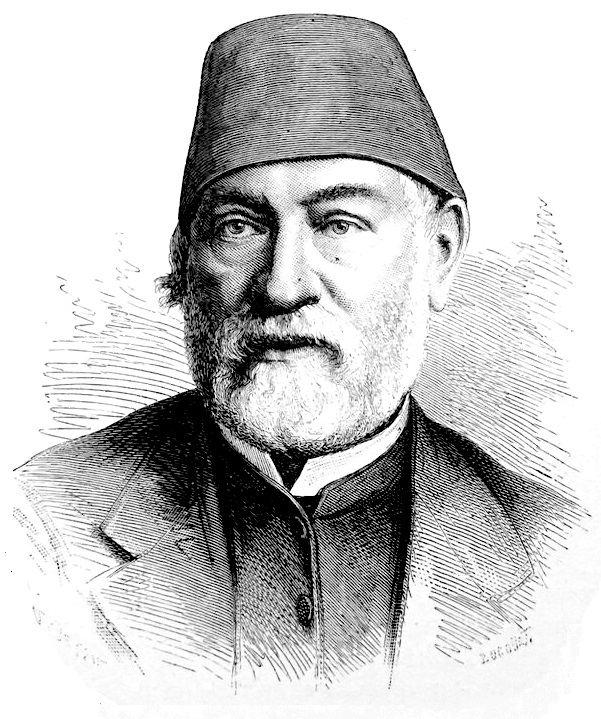
\includegraphics[height=12cm]{CoEg_Mariette_portrait.jpg}
\vfill
\hspace{0pt}

\pagebreak


\LARGE{C O R R E S P O N D A N C E S}
    
\Huge{É G Y P T O L O G I Q U E S}
\vspace{1\baselineskip}

\large C O N T E N A N T\space\space\space D E S
\vspace{1\baselineskip}

\Large L E T T R E S\space\space\space D ’ É G Y P T O L O G U E S
\vspace{2\baselineskip}

\large dispersées dans diverses institutions
\vspace{1\baselineskip}

et qui n’ont pas encore été rassemblées jusqu’à ce jour
\vspace{9\baselineskip}

\LARGE L E T T R E S\space\space\space D\space ’\space A U G .\space\space\space M A R I E T T E
\vspace{4\baselineskip}

\normalsize É D I T É E S\space\space\space P A R \space\space\space T H .\space\space\space L E B É E
\vspace{4\baselineskip}

Version 0,18 bis
\vspace{1\baselineskip}

Juin 2020
\end{titlepage}

\frontmatter

\chapter*{Introduction}
\addcontentsline{toc}{chapter}{Introduction}

\section*{Le projet des \textit{Correspondances égyptologiques}}
\addcontentsline{toc}{section}{Le projet des Correspondances égyptologiques}

Ce fichier résulte d’un projet personnel d’édition numérique des lettres écrites par l’égyptologue Auguste Mariette. Il s’agit d’une initiative dont l’objectif est de rendre librement accessibles ces documents et de permettre leur exploitation scientifique.
\par Le corpus édité ici a vocation à intégrer chaque lettre repérée de Mariette. Les brouillons de lettres seront aussi incorporés, dans la mesure où il n’est pas toujours possible d’établir si une lettre a véritablement été transmise à son destinataire et que les hésitations et repentirs de la rédactions peuvent être riches d’enseignements.
\par L’édition des lettres sera progressive, afin de publier les documents régulièrement et d’en améliorer le format au moyen des suggestions qui pourront être recueillies au cours de l’entreprise. Les sources parisiennes seront dépouillées en priorité pour commencer (par pure commodité matérielle), mais bien d’autres devraient suivre.
\par Les publications successives du corpus sont disponibles sur le site \href{https://thlebee.github.io/CoEg_test_forty/}{\textit{Correspondances égyptologiques}}, à la fois au format XML-TEI et en une version PDF réalisée au moyen de Latex (que vous consultez en ce moment). Les métadonnées du corpus sont aussi disponibles. Chaque enrichissement sera signalé sur le carnet de recherche \href{https://hef.hypotheses.org/}{\textit{Histoire de l’égyptologie en formation}}.
\par Toute remarque, critique ou suggestion d’amélioration sera la bienvenue à l’adresse suivante~: \href{mailto:correspondances.egyptologiques@laposte.net}{correspondances.egyptologiques@laposte.net} (merci également d’y signaler toute utilisation qui pourra être faite de ces ressources, à titre d’information).
\par Le contenu de ce document est publié sous licence CC-BY~: toute réutilisation en est permise, et encouragée~– sous réserve de la mention de la source (par exemple~: «~Auguste Mariette (Thomas Lebée, éd.), \textit{Correspondances égyptologiques. Lettres d’Auguste Mariette}~»).

\section*{Encodage et principes éditoriaux}
\addcontentsline{toc}{section}{Encodage et principes éditoriaux}

\par L’encodage résulte de plusieurs étapes, destinées à transcrire le document tel qu’il apparaît, puis à baliser ses composants structurels et un certain nombre de termes d’indexations.
\par Le corpus édité ici a vocation à intégrer chaque lettre repérée de Mariette. Les brouillons de lettres seront aussi incorporés, dans la mesure où il n’est pas toujours possible d’établir si une lettre a véritablement été transmise à son destinataire et que les hésitations et repentirs de la rédactions peuvent être riches d’enseignements.
\par Chaque lettre a été considérée comme une unité documentaire distincte, dont les références bibliographiques et administratives sont rappelées en tête de notice, avec le cas échéants toutes remarques jugées utile à sa compréhension. Les lettres peuvent dès lors être arrangées dans l’ordre chronologique pour retrouver leur continuité malgré la dispersion des fonds.
\par La ponctuation de Mariette a été conservée sans modification autant qu’elle était lisible. Pour être compréhensibles, les signes de ponctuation barrés ont parfois été remplacés par leur description entre crochets.
\par Cette édition recherche la plus grande fidélité au texte de Mariette. Les graphies variables des noms propres et l’absence d’accents sur les majuscules ont ainsi été conservées telles quelles. Les fautes d’orthographe, systématiques ou incidentes, ont également été conservées, et marquées par un balisage aproprié dès lors qu’elles s’éloignaient de l’orthographe et de l’usage contemporain. Toute intervention ou doute dans la lecture du texte manuscrit est signalée explicitement par le balisage ou la ponctuation.
\par La copie numérique, comme la transcription par des caractères mécaniques, comporte cependant une part d’interprétation et de standardisation. Puisqu’il s’agissait de reproduire un texte manuscrit en caractères typographiques, les codes habituels ont été appliqués~: le texte souligné à la main a été rendu en italiques, le double soulignement par de petites capitales et les guillemets ont systématiquement été transcrits comme des guillemets typographiques (en chevrons).
\par L’écriture de Mariette n'est pas des plus régulières et les hampes de ses lettres sont parfois trompeuses. En cas de doute entre une majuscule ou une minuscule, ou même sur l’orthographe utilisée, la graphie régulière a été privilégiée en l’absence d’erreur manifeste. Les lectures hasardeuses sont signalées par le balisage, mais il est aussi à noter que les mots courts sont régulièrement hasardeux. Si le contexte permet d’en confirmer la plupart, certaines distinctions restent largement conjecturales (notamment la différence entre «~notre~»/«~votre~» et «~nos~»/«~vos~»). Les ratures ont été déchiffrées dans la mesure du possible, ou juste indiquées en tant que telles.

\section*{Le corpus}
\addcontentsline{toc}{section}{Le corpus}
\subsection*{Archives nationales}
\addcontentsline{toc}{subsection}{Archives nationales}
\subsubsection*{20150497/118, dossier 145}
\addcontentsline{toc}{subsubsection}{20150497/118, dossier 145}
\label{CoEg_Mariette_ms_001}
\noindent Ancienne cote : Paris, Bibliothèque centrale des musées nationaux, O/30/145 (cote utilisée avant le versement aux Archives nationales en 2015).
\begin{itemize}
\item \nameref{CoEg_Mariette_1851-02-28} ;
\item \nameref{CoEg_Mariette_1851-08-31} ;
\item \nameref{CoEg_Mariette_1852-01-16} ;
\item \nameref{CoEg_Mariette_1852-08-04} ;
\item \nameref{CoEg_Mariette_1852-08-20} ;
\item \nameref{CoEg_Mariette_1852-09-03} ;
\item \nameref{CoEg_Mariette_1852-09-04} ;
\item \nameref{CoEg_Mariette_1852-11-12} ;
\item \nameref{CoEg_Mariette_1852-12-28} ;
\item \nameref{CoEg_Mariette_1853-01-01} ;
\item \nameref{CoEg_Mariette_1853-05-06} ;
\item \nameref{CoEg_Mariette_1853-07-30} ;
\item \nameref{CoEg_Mariette_1853-08-10} ;
\item \nameref{CoEg_Mariette_1853-08-28} ;
\item \nameref{CoEg_Mariette_1857-10-26} ;
\item \nameref{CoEg_Mariette_1857-11-29} ;
\item \nameref{CoEg_Mariette_1858-01-23} ;
\item \nameref{CoEg_Mariette_1860-12-20}.
\end{itemize} \par
Ces lettres ont été conservées dans le dossier personnel de Mariette\gls{CoEg_pers_00000001} au sein des archives de l'administration des musées nationaux\gls{CoEg_org_00000001}. Elles forment trois groupes inégaux correspondant à plusieurs étapes de la carrière de Mariette\gls{CoEg_pers_00000001} et à ses voyages successifs en Égypte\gls{CoEg_place_00000003}. Malgré leur cordialité de ton et quelques anecdotes, il s’agit ainsi surtout d’une correspondance professionnelle, dans laquelle l’égyptologue évoque les progrès de ses missions et ses préoccupations en ce qui concerne l’entretien matériel de sa famille.\par
Les quatorze premières lettres datent du premier voyage de Mariette\gls{CoEg_pers_00000001} en Égypte\gls{CoEg_place_00000003} (1850-1853). Les lettres concernent surtout les communications entre Mariette\gls{CoEg_pers_00000001} en mission et son autorité de tutelle, pour l’informer de la situation du terrain, réclamer périodiquement des fonds et demander des directives ou expliquer ses initiatives. Les négociations avec le gouvernement égyptien\gls{CoEg_org_00000008}, les stratagèmes de Mariette\gls{CoEg_pers_00000001} pour interpréter très libéralement les accords conclus avec celui-ci (ou le contourner tout à fait) et la coordination de ses efforts avec ceux du ministère des Affaires étrangères\gls{CoEg_org_00000007}, par le truchement du consulat général\gls{CoEg_org_00000006} de France\gls{CoEg_place_00000016} à Alexandrie\gls{CoEg_place_00000006} sont les principaux objets de ces lettres, qui renferment également des indications précises sur l’avancée des fouilles et quelques détails de sa vie quotidienne.\par
Trois lettres datent du second voyage en Égypte\gls{CoEg_place_00000003} de Mariette\gls{CoEg_pers_00000001} (1857-1858). Elles traitent surtout de la préparation du voyage du prince Napoléon\gls{CoEg_pers_00000074}, prétexte officiel à cette nouvelle mission, qui n’eut finalement pas lieu ; de l’annonce par Mariette\gls{CoEg_pers_00000001} d’acquisitions destinées au prince, mais dont il espère qu’elles rejoindront le Louvre\gls{CoEg_org_00000002} ; et enfin de la régularisation de ses congés prolongés le temps de la mission, afin qu'il puisse rester éloigné du Louvre\gls{CoEg_org_00000002} sans déroger au règlement et que sa famille touche ses appointements.\par
La dernière lettre, du 20 décembre 1860, est la réponse à celle envoyée à Mariette\gls{CoEg_pers_00000001} par Nieuwerkerke\gls{CoEg_pers_00000002} le 29 novembre (conservée dans le dossier et transcrite en note) et dans laquelle il lui annonçait être contraint de nommer un conservateur adjoint à sa place, et le nommait lui-même conservateur adjoint honoraire, Mariette\gls{CoEg_pers_00000001} se trouvant alors déjà engagé au service du vice-roi\gls{CoEg_pers_00000080} d’Égypte\gls{CoEg_place_00000003} pour diriger le service des antiquités.\par
Trois de ses lettres sont destinées au ministre de l’Intérieur (dont dépendaient les musées nationaux\gls{CoEg_org_00000001} jusqu’en 1852) ; sept s’adressent au directeur du musée du Louvre\gls{CoEg_org_00000002}, le comte de Nieuwerkerke\gls{CoEg_pers_00000002} ; enfin, le destinataire de neuf d’entre elles n’est pas explicitement nommé, mais il s’agissait manifestement d’un fonctionnaire parisien en relation avec les autres administrations et qui fréquentait les collègues de Mariette\gls{CoEg_pers_00000001} au Louvre\gls{CoEg_org_00000002} : il est très probable qu’il s’agisse là aussi du comte de Nieuwerkerke\gls{CoEg_pers_00000002}.\par
Ces archives originellement conservées à la bibliothèque centrale des musées nationaux ont été versées aux Archives nationales en 2015.

\section*{Historique du fichier}
\addcontentsline{toc}{section}{Historique du fichier}
\begin{itemize}
\item Février 2020 : v. 0,18 : essais sur un premier échantillon de lettres issus du dossier de carrière de Mariette\gls{CoEg_pers_00000001} dans l'administration des musées nationaux\gls{CoEg_org_00000001}.
\item Juin 2020 : v. 0,18 bis : toujours sur le même corpus restreint, essai de traitement complet de l'ensemble documentaire selon une procédure plus cadrée et essais de publications sur \href{https://thlebee.github.io/CoEg_test_forty/}{GitHub}.
\end{itemize}

\mainmatter

\chapter*{Lettres d'Auguste Mariette}
\addcontentsline{toc}{chapter}{Lettres d'Aug. Mariette}
\section*{Le 28 février 1851, de Saqqara, à Nieuwerkerke} \label{CoEg_Mariette_1851-02-28} \addcontentsline{toc}{section}{Le 28 février 1851, de Saqqara, à Nieuwerkerke}
{\footnotesize
\noindent Institution et lieu de conservation : Archives nationales\gls{CoEg_org_00000024}, Pierrefitte-sur-Seine.\\
Cote : \hyperref[CoEg_Mariette_ms_001]{20150497/118}, dossier 145 (Mariette, Auguste), lettre s. n.\\
Support : 1 feuille double.
\begin{center} {[1\textsuperscript{re} page, r\textsuperscript{o}]}\end{center}}
\noindent [Donné par\\
M Maspero ?]\footnote{Courtes annotations au crayon, de lecture très incertaine, au coin supérieur gauche de la page.}
\begin{flushright}
Saqqarah\gls{CoEg_place_00000001}, le 28 février 1851.
\end{flushright}
A Monsieur
\begin{center} Monsieur le Directeur des Musées Nationaux\gls{CoEg_org_00000001}\end{center}
\begin{flushright}à Paris\gls{CoEg_place_00000002}.\end{flushright}

\hspace{1cm} Monsieur le Directeur\gls{CoEg_pers_00000002},\\

\par Au mois d’Août de l’année passée, vous avez bien voulu m’accorder\\
un congé de six mois.\\
\indent L’espoir que la mission qui m’a été confiée par \gls{CoEg_abbr_00000001} le Ministre de
\\l’Instruction Publique\gls{CoEg_pers_00000003} et \gls{CoEg_abbr_00000001} le Ministre de l’Intérieur\gls{CoEg_pers_00000004} aurait pour\\
résultat l’accroissement des Antiquités Egyptiennes du Louvre\gls{CoEg_org_00000002}, vous a\\
décidé à me faire une faveur dont je vous suis reconnaissant.\\
\indent Mais ce congé expire le 31 mars prochain, et à cette époque je\\
serai encore en Egypte\gls{CoEg_place_00000003} pour deux mois au moins.\\
\indent Vous me rendriez donc un nouveau service, Monsieur le Directeur,\\
si vous vouliez prolonger la permission d’absence que vous m’avez donnée\\
jusqu’à la fin du mois de mai, c’est-à-dire pendant deux nouveaux\\
mois.\\
\indent Je vous demanderai aussi de m’accorder pour le même temps mes\\
appointements ordinaires. S’il m’était permis de faire intervenir dans\\
cette affaire des questions toutes personnelles, je vous rappellerais\\
que je ne suis pas riche, et qu’en mon absence les deux mois\\
d’appointements que je sollicite de vous sont le seul moyen que\\
j’aie de subvenir aux besoins de ma famille\footnote{La famille Mariette est alors composée de son épouse Éléonore (née Millon)\gls{CoEg_pers_00000005} et leurs filles Marguerite Louise\gls{CoEg_pers_00000006}, Joséphine Cornélie\gls{CoEg_pers_00000007}, Sophie Éléonore\gls{CoEg_pers_00000008}.} que j’ai laissée à Paris\gls{CoEg_place_00000002}.\\
\indent J’attends donc de votre justice et de l’intérêt si vif que vous\\
m’avez souvent témoigné le double service que j’ai l’honneur de\\
solliciter de vous.
\begin{flushright}Je vous dirai\end{flushright}
{\footnotesize \begin{center} {[1\textsuperscript{re} page, v\textsuperscript{o}]}\end{center}}
\indent Je vous dirai d’ailleurs que si, contre toutes mes prévisions, je reste\\
en Egypte\gls{CoEg_place_00000003} plus long-temps que je ne le pensais, chaque jour de\\
retard apporte au Louvre\gls{CoEg_org_00000002} un monument nouveau. Le hasard\\
m’a en effet réservé une des plus curieuses découvertes de l’archéologie\\
Egyptienne. Quatre mois me séparent déjà du premier jour où je\\
tentai mes premiers essais pour retrouver le Sérapéum\gls{CoEg_place_00000004} de Memphis\gls{CoEg_place_00000005},\\
et les deux autres mois que je vous prie de m’accorder ne me mèneront\\
tout au plus qu’à la moitié des travaux qu’il faudrait faire pour\\
épuiser la mine si riche en monuments de toute espèce que j’ai\\
trouvée.\\
\indent Pour vous en convaincre, Monsieur le Directeur, je vous dirai que,\\
\textit{dès maintenant}, je tiens à votre disposition \textit{comme monuments\\
principaux} :\\
\indent 1.160 = De 150 à 160 sphinx en grès, de la grandeur de ceux de\\
Néphéritès\gls{CoEg_pers_00000009} au Louvre\gls{CoEg_org_00000002}\footnote{Le musée du Louvre conserve deux sphinx tardifs dont l'un (A 26\gls{CoEg_obj_00000001}) est inscrit au nom de Néphéritès I\textsuperscript{er}\gls{CoEg_pers_00000009}.} ; j’en emporterai le nombre que vous voudrez bien\\
m’indiquer, et, en attendant, j’en ai choisi six\gls{CoEg_obj_00000002} qui vont bientôt\\
partir pour Alexandrie\gls{CoEg_place_00000006} ;\\
\indent 161 = un sphinx plus grand avec les légendes d’Amyrtés\gls{CoEg_pers_00000010} ; ce roi\\
n’est pas, je crois, représenté au Louvre\gls{CoEg_org_00000002} ;\\
\indent 162-163 = deux très-beaux bas-reliefs représentant Amyrtés\gls{CoEg_pers_00000010}\\
en adorateur devant Apis\gls{CoEg_pers_00000011} ;\\
\indent 164 = une base en grès, commune à deux statues en basalte, avec\\
dix-neuf lignes en démotique ;\\
\indent 165 = une statue de grandeur naturelle du Dieu Typhon\gls{CoEg_pers_00000012} ;\\
\indent 166 à 176 = onze statues \textit{grecques} plus ou moins mutilées ; l’une\\
d’elles, d’une conservation assez remarquable, représente un personnage\\
assis, et portant sur l’épaule gauche ce qu’il m’est impossible
{\footnotesize \begin{center} {[2\textsuperscript{e} page, r\textsuperscript{o}]}\end{center}}
\noindent de ne pas prendre pour une colonne vertébrale humaine ;\\
\indent 177 = un groupe colossal de style grec représentant un\\
jeune homme à cheval sur un \textit{monstre} à tête humaine, à corps de\\
chien, à pattes de lion et à griffes d’aigle ;\\
\indent 178 = 179 = deux groupes représentant, chacun, un enfant\\
à cheval sur un \textit{paon} ; la queue de l’animal, développée\\
derrière lui, forme une roue qui a plus de six pieds de diamètre ;\\
\indent 180 = une stèle\gls{CoEg_obj_00000003}, trouvée encore en place à l’entrée du Sérapéum\gls{CoEg_place_00000004},\\
et représentant Nectanébo\gls{CoEg_pers_00000013} en adoration devant neuf divinités en\\
tête desquelles figure la triade thébaine ;\\
\indent 181.182 \footnote{Mariette\gls{CoEg_pers_00000001} a d’abord écrit \og 181 = \fg puis a barré l’égal et ajouté \og .182 \fg par-dessus.} = deux \textit{magnifiques lions}\footnote{Le Louvre obtint finalement trois de ces lions, conservés sous les numéros d'inventaire N 432 A\gls{CoEg_obj_00000004} (sous lequel était encastré la stèle C 318\gls{CoEg_obj_00000003}), N 432 A\gls{CoEg_obj_00000005} et N 432 A\gls{CoEg_obj_00000006}.}, d’une conservation admirable,\\
qui sont la reproduction \textit{très-exacte} de ceux du Vatican\gls{CoEg_org_00000003} dont des\\
moulages de bronze servent de fontaines devant le Palais de l’Institut\gls{CoEg_org_00000004}\\
à Paris\gls{CoEg_place_00000002} ;\\
\indent 183 = un sarcophage rectangulaire que j’ai rencontré par hasard\\
dans mes fouilles ; il reproduit à l’extérieur l’ornementation\\
du cercueil de la 3\textsuperscript{e} pyramide de Gyzeh\gls{CoEg_place_00000007}, et offre cet intérêt particulier\\
qu’il n’a jamais été achevé ; d’un côté les sculptures sont parfaites,\\
de l’autre elles ne sont qu’ébauchées à grands traits ; quelques\\
figures sont simplement dessinées à l’ocre rouge ; la plupart\\
des légendes sont aussi en [rature] ocre rouge ; on y remarque des\\
corrections, des additions tracées en surcharge avec de l’encre noire.\\
\indent Ces monuments, Monsieur le Directeur, ne sont que les\\
principaux de ceux que j’ai trouvés. Je vous les cite parce que je\\
les ai tous vus et dessinés. D’un autre côté mes fouilles ne sont\\
pas encore à leur première moitié, puisque je suis à peine entré\\
dans le Sérapéum\gls{CoEg_place_00000004}. Il y a une huitaine de jours, des fouilles
\begin{flushright}partielles\end{flushright}
{\footnotesize \begin{center} [2\textsuperscript{e} page, v\textsuperscript{o}]\end{center}}
\noindent partielles m’ont révélé la place de huit autres groupes de style\\
grec (l’un d’entre eux représente un enfant à cheval sur un coq),\\
et de onze stèles en place, dont trois, m’ont assuré mes Arabes,\\
sont en basalte. Je n’ai pas introduit ces monuments dans la\\
liste qui précède, parce que je n’ai pas pu les bien voir. Un\\
accident trop fréquent dans les sables du désert de Saqqarah\gls{CoEg_place_00000001} a\\
en effet bouleversé tout le Sérapéum\gls{CoEg_place_00000004} ; pendant trois jours le\\
\Gls{CoEg_term_00000001} a soufflé avec une telle violence que toutes mes excavations\\
ont été bouchées, mes tentes enlevées dans les airs, et que depuis\\
cinq jours, je n’ai pu encore réparer les désastres de cette tempête.\\
\indent Mais quoi qu’il en soit, ce que j’ai déjà et dont je vous ai donné\\
une liste très-sommaire, vous fait assez voir qu’en vous demandant\\
de m’accorder mes appointements pendant deux nouveaux mois,\\
je vous offre en retour des compensations plus que suffisantes.\\
\indent Permettez-moi donc d’espérer, Monsieur le Directeur, que vous\\
ne vous refuserez pas à faciliter, autant que vous le pouvez,\\
des recherches que je poursuis moi-même avec toute la persévérance\\
dont je suis capable et que je n’abandonnerai que lorsque les\\
chaleurs rendront impossibles le travail des sables du désert.
\par J’ai l’honneur d’être,
\begin{center} Monsieur le Directeur,\end{center}
\begin{center} \hspace{5cm}Votre très-humble\\
\hspace{5cm}et très-obéissant serviteur\\
\hspace{5cm} \gls{CoEg_abbr_00000002} Mariette\end{center}
\section*{Le 31 août 1851, de Saqqara, à Nieuwerkerke} \label{CoEg_Mariette_1851-08-31} \addcontentsline{toc}{section}{Le 31 août 1851, de Saqqara, à Nieuwerkerke}
{\footnotesize
\noindent Institution et lieu de conservation : Archives nationales\gls{CoEg_org_00000024}, Pierrefitte-sur-Seine\\
Cote : \hyperref[CoEg_Mariette_ms_001]{20150497/118}, dossier 145 (Mariette, Auguste), lettre s. n.\\
Support : 1 feuille double.\\
Note : une copie non datée de cette lettre se trouve dans les papiers Mariette\gls{CoEg_pers_00000001} conservés au sein du fonds Maspero à la bibliothèque de l'Institut de France\gls{CoEg_org_00000004} (ms. 4061 (2), f\textsuperscript{os} 11-13 pour cette lettre), parmi la copie de douze de ses lettres dont la plupart sont issues de son dossier personnel de l'administration des musées nationaux (aujourd'hui aux Archives nationales\gls{CoEg_org_00000024} sous la cote \hyperref[CoEg_Mariette_ms_001]{20150497/118}, dossier 145), et de sept lettres envoyées par lui à Kabis\gls{CoEg_pers_imn} (aujourd'hui aux Archives nationales\gls{CoEg_org_00000024} aussi sous la cote AB/XIX/4195). Ces copies ne sont pas de la main de Mariette\gls{CoEg_pers_00000001}, mais correspondent à une écriture ancienne (parmi elles, la lettre la plus récente est de 1869) ; leur interprétation n'est d'ailleurs pas toujours très fiable.
\begin{center} {[1\textsuperscript{re} page, r\textsuperscript{o}]}\end{center}}
\begin{flushright}Saqqarah\gls{CoEg_place_00000001}, le 31 août 1851.\end{flushright}
A Monsieur
\begin{center}Monsieur le Directeur des Musées Nationaux\gls{CoEg_org_00000001}\end{center}
\begin{flushright}à Paris\gls{CoEg_place_00000002}.\end{flushright}

\indent \hspace{1cm}Monsieur le Directeur\gls{CoEg_pers_00000002},\\

J’ai reçu en son temps votre lettre du 17 avril. Mais atteint alors\\
d’une ophtalmie qui me privait de l’usage de mes yeux, je n’ai pu\\
prendre connaissance de cette lettre que le 4 Juin suivant.\\
\indent Le 6 Juin j’envoyai au Caire\gls{CoEg_place_00000010} un exprès chargé – ou de rencontrer\\
\gls{CoEg_abbr_00000001} Lafuente\gls{CoEg_pers_00000014} et de lui remettre un mot de moi – ou de chercher à savoir\\
où il se trouvait.\\
\indent Malheureusement \gls{CoEg_abbr_00000001} Lafuente\gls{CoEg_pers_00000014} était alors à Londres\gls{CoEg_place_00000011}, et ce n’est\\
qu’au commencement de ce mois que j’appris son retour à Alexandrie\gls{CoEg_place_00000006}, sa\\
résidence ordinaire.\\
\indent Je lui écrivis immédiatement dans le sens de vos instructions. Je lui\\
demandai :\\
\indent \gls{CoEg_abbr_00000005} le prix de \gls{CoEg_abbr_00000001} d’Anastasy\gls{CoEg_pers_00000015} pour la partie de la collection égyptienne\\
de Livourne\gls{CoEg_place_00000012}, qui comprend les stèles ;\\
\indent \gls{CoEg_abbr_00000006} le prix de la seconde partie qui comprend les papyrus ;\\
\indent \gls{CoEg_abbr_00000007} enfin le prix des deux sections réunies.\\
\indent J’ai reçu il y a peu de jours la réponse de \gls{CoEg_abbr_00000001} Lafuente\gls{CoEg_pers_00000014} – \gls{CoEg_abbr_00000001}\\
d’Anastasy\gls{CoEg_pers_00000015} consent à couper sa collection, non pas en trois, mais
{\footnotesize \begin{center} [1\textsuperscript{re} page, v\textsuperscript{o}]\end{center}}
\noindent en deux ; il distrait du tout les \textit{bijoux} et les \textit{scarabées}, et demande\\
du reste 80,000 francs.\\
\indent J’ai l’honneur, Monsieur le Directeur, de vous soumettre les\\
propositions de \gls{CoEg_abbr_00000001} d’Anastasy\gls{CoEg_pers_00000015}, et dans le cas où vous auriez\\
de nouvelles instructions à me donner, je suis naturellement\\
à vos ordres.\\
\indent Je\footnote{Mariette\gls{CoEg_pers_00000001} a d'abord écrit \og J' \fg puis a barré l'apostrophe.} dois ajouter que j’avais profité de mes bonnes relations avec\\
\gls{CoEg_abbr_00000001} Lafuente\gls{CoEg_pers_00000014} pour le prier officieusement d’intervenir dans cette\\
affaire, en usant de son influence sur \gls{CoEg_abbr_00000001} d’Anastasy\gls{CoEg_pers_00000015} pour\\
engager celui-ci – soit à vous offrir un prix plus raisonnable\\
de la collection – soit à choisir le Louvre\gls{CoEg_org_00000002}, dans le cas où il\\
se déciderait définitivement à faire don de cette même collection\\
à l’un des Musées de l’Europe\gls{CoEg_place_00000013}.\\
\indent Sur la première de ces deux questions, \gls{CoEg_abbr_00000001} Lafuente\gls{CoEg_pers_00000014} me fait\\
savoir que les 80,000 francs ne représentent pas le prix définitif de\\
la collection, mais qu’il semble à \gls{CoEg_abbr_00000001} d’Anastasy\gls{CoEg_pers_00000015} que c’est sur\\
cette première base que peuvent commencer les pourparlers.\\
\indent Sur le second point, \gls{CoEg_abbr_00000001} Lafuente\gls{CoEg_pers_00000014} ne se prononce aucunement.\\
Je n’aurai donc rien à ajouter à ce que je vous ai déjà dit à\\
ce sujet, puisque je ne sais pas mieux qu’avant si \gls{CoEg_abbr_00000001}\\
d’Anastasy\gls{CoEg_pers_00000015} veut réellement doter l’un des établissements scientifiques\\
de l’Europe\gls{CoEg_place_00000013} des richesses archéologiques qu’il a réunies à\\
Livourne\gls{CoEg_place_00000012}, ou si, en parlant à tout le monde du plaisir\\
qu’il aurait à attacher son nom à une belle collection, il ne\\
veut pas se donner à lui-même l’honneur d’une intention\\
généreuse. Cependant, Monsieur le Directeur, si vous voulez\\
bien me permettre de vous exprimer mon opinion personnelle
{\footnotesize \begin{center} [2\textsuperscript{e} page, r\textsuperscript{o}]\end{center}}
\noindent je vous dirai que, pour le [moment ?], toutes les distinctions honorifiques\\
dont vous pouvez disposer ne tenteront pas \gls{CoEg_abbr_00000001} d’Anastasy\gls{CoEg_pers_00000015}.\\
\indent \gls{CoEg_abbr_00000001} d’Anastasy\gls{CoEg_pers_00000015} n’est en effet consul-général de Suède\gls{CoEg_place_00000014} que\\
pour l’honneur de ce titre. Négociant et banquier de Son Altesse\\
le Vice-Roi\gls{CoEg_pers_00000016}, il est ce qu’on appelle un homme d’argent, et\\
par conséquent de ceux que n’éblouissent pas les distinctions\\
honorifiques. En [rature] général, \gls{CoEg_abbr_00000001} d’Anastasy\gls{CoEg_pers_00000015} ne donnerait donc\\
la collection de Livourne\gls{CoEg_place_00000012}, que s’il lui devient bien prouvé qu’il ne\\
peut la vendre.\\
\indent Je dirai de plus que, dans les circonstances actuelles, \gls{CoEg_abbr_00000001}\\
d’Anastasy\gls{CoEg_pers_00000015} est moins porté que jamais à céder à un mouvement\\
de générosité. Permettez-moi, pour être clair, de vous parler en\\
insistant le langage familier du Caire\gls{CoEg_place_00000010}. En ce moment, les choses\\
{[s’arrangent ?]} ainsi en Egypte\gls{CoEg_place_00000003} que, de quelque nation que l’on\\
soit, on n’est jamais qu’\textit{anglais} ou \textit{français}. Ces [discriminations ?],\\
pour ceux qui voient de près les affaires publiques de ce pays,\\
indiquent de la manière la plus expressive les deux extrêmes qui\\
sont en présence. Méhémet-Ali\gls{CoEg_pers_00000017} était \textit{français} ; Abbas-\Gls{CoEg_term_00000002}\gls{CoEg_pers_00000016}\\
est \textit{anglais}. Le premier faisait de la France\gls{CoEg_place_00000016} son alliée ; il\\
appelait des français au gouvernement de l’Egypte\gls{CoEg_place_00000003} ; Abbas-\Gls{CoEg_term_00000002}\gls{CoEg_pers_00000016}\\
les congédie, un à un et systématiquement. C’est ainsi que\\
Linant-\gls{CoEg_term_00000003}\gls{CoEg_pers_00000019}, Lambert-\gls{CoEg_term_00000003}\gls{CoEg_pers_00000020}, Clot-\gls{CoEg_term_00000003}\gls{CoEg_pers_00000021}, Varin-\gls{CoEg_term_00000003}\gls{CoEg_pers_00000022} sont en disgrâce,\\
tandis que le Vice-Roi\gls{CoEg_pers_00000016} actuel élève aux hautes fonctions des\\
sujets anglais. Il est vrai qu’il n’a encore fait qu’un \gls{CoEg_term_00000003}\\
anglais, et que ce \gls{CoEg_term_00000003} est son \textit{boulanger}. Il s’appelle\\
Walker-\gls{CoEg_term_00000003}\gls{CoEg_pers_00000023}.\\
\indent Quoi qu’il en soit, les deux systèmes sont aujourd’hui\\
parfaitement définis et il ne faut pas être venu deux fois\\
au Caire\gls{CoEg_place_00000010} pour s’apercevoir que rien n’est plus exact que les\\
deux grandes divisions qui partagent les colonies européennes
de l’Egypte\gls{CoEg_place_00000003}.
{\footnotesize \begin{center} [2\textsuperscript{e} page, v\textsuperscript{o}]\end{center}}
\indent Or \gls{CoEg_abbr_00000001} d’Anastasy\gls{CoEg_pers_00000015} est Anglais. Et il l’est d’autant plus en\\
ce moment que, banquier de \gls{CoEg_abbr_00000003}\gls{CoEg_pers_00000016}, il va être pour beaucoup dans\\
la grande entreprise de Chemin de fer d’Alexandrie\gls{CoEg_place_00000006} au Caire\gls{CoEg_place_00000010} qui\\
vient d’être concédé à une compagnie anglaise sur la demande\\
expresse de \gls{CoEg_abbr_00000001} Murray\gls{CoEg_pers_00000018}, consul-général d’Angleterre\gls{CoEg_place_00000015}.\\
\indent Dans les circonstances présentes, il me semble donc que vous n’avez\\
guère à espérer de \gls{CoEg_abbr_00000001} d’Anastasy\gls{CoEg_pers_00000015} le don, à titre gratuit, de\\
sa magnifique collection de Livourne\gls{CoEg_place_00000012}. J’ai la conviction que,\\
s’il la donnait à quelqu’un, ce serait au Musée Britannique\gls{CoEg_org_00000005}.\\
\indent Mais je crois qu’il y aurait peut-être, plus tard, un moyen\\
d’obtenir ce cadeau ; ce serait celui d’\textit{attendre}. On parle en effet\\
du remplacement de \gls{CoEg_abbr_00000001} Lemoyne\gls{CoEg_pers_00000024}, notre consul-général, par \gls{CoEg_abbr_00000001}\\
Benedetti\gls{CoEg_pers_00000025} – Or \gls{CoEg_abbr_00000001} Benedetti\gls{CoEg_pers_00000025} est le gendre de \gls{CoEg_abbr_00000001} d’Anastasy\gls{CoEg_pers_00000015}.\\
\indent Je vous transmets, Monsieur le Directeur, ces renseignements pour\\
vous éclairer dans la décision que \textsuperscript{vous} voudrez bien prendre. Je n’ai plus\\
maintenant qu’à attendre vos ordres.\\
\indent J’ajouterai que, connaissant le caractère et la situation présente\\
de \gls{CoEg_abbr_00000001} d’Anastasy\gls{CoEg_pers_00000015}, j’aurai peut-être dû m’abstenir d’entamer les\\
négociations dont vous m’avez chargé ; pour obtenir un cadeau de\\
\gls{CoEg_abbr_00000001} d’Anastasy\gls{CoEg_pers_00000015}, il ne faut pas en effet commencer par lui laisser\\
voir qu’on est disposé à acheter. Mais j’ai cru devoir parler haut\\
de l’argent du Louvre\gls{CoEg_org_00000002}, et je pense que traîner les pourparlers en\\
longueur est le seul moyen que nous ayons d’empêcher \gls{CoEg_abbr_00000001}\\
d’Anastasy\gls{CoEg_pers_00000015} de céder aux obsessions de quelques personnes et\\
d’honorer de sa générosité un autre établissement que le Louvre\gls{CoEg_org_00000002}.\\
Je vous répète en effet que tant que \gls{CoEg_abbr_00000001} d’Anastasy\gls{CoEg_pers_00000015} croira\\
que le Louvre\gls{CoEg_org_00000002} veut acheter, il ne donnera à personne, pas même\\
au Musée Britannique\gls{CoEg_org_00000005}.\\
\indent J’ai l’honneur d’être,
\begin{center}Monsieur le Directeur,\end{center}
\begin{center}\hspace{5cm}Votre très-humble serviteur.\\
\hspace{5cm}\gls{CoEg_abbr_00000002} Mariette\end{center}
\noindent \gls{CoEg_abbr_00000008} Je continue à être satisfait de\\
mes fouilles. Le Sérapéum\gls{CoEg_place_00000004} de Memphis\gls{CoEg_place_00000005}\\
a été décidément construit par Ramsès II\gls{CoEg_pers_00000026}.\\
Quelques parties \textit{grecques} sont du temps de Nectanébo\gls{CoEg_pers_00000013}.
\section*{Le 16 janvier 1852, d'Abousir, à [Nieuwerkerke]} \label{CoEg_Mariette_1852-01-16} \addcontentsline{toc}{section}{Le 16 janvier 1852, d'Abousir, à [Nieuwerkerke]}
{\footnotesize
\noindent Institution et lieu de conservation : Archives nationales\gls{CoEg_org_00000024}, Pierrefitte-sur-Seine\\
Cote : \hyperref[CoEg_Mariette_ms_001]{20150497/118}, dossier 145 (Mariette, Auguste), lettre s. n.\\
Support : 1 feuille double.\\
Note : une copie non datée de cette lettre se trouve dans les papiers Mariette\gls{CoEg_pers_00000001} conservés au sein du fonds Maspero à la bibliothèque de l'Institut de France\gls{CoEg_org_00000004} (ms. 4061 (2), f\textsuperscript{os} 20-23 pour cette lettre), parmi la copie de douze de ses lettres dont la plupart sont issues de son dossier personnel de l'administration des musées nationaux (aujourd'hui aux Archives nationales\gls{CoEg_org_00000024} sous la cote \hyperref[CoEg_Mariette_ms_001]{20150497/118}, dossier 145), et de sept lettres envoyées par lui à Kabis\gls{CoEg_pers_imn} (aujourd'hui aux Archives nationales\gls{CoEg_org_00000024} aussi sous la cote AB/XIX/4195). Ces copies ne sont pas de la main de Mariette\gls{CoEg_pers_00000001}, mais correspondent à une écriture ancienne (parmi elles, la lettre la plus récente est de 1869) ; leur interprétation n'est d'ailleurs pas toujours très fiable.
\begin{center} {[1\textsuperscript{re} page, r\textsuperscript{o}]}\end{center}}
\begin{flushright}Du désert d’Abousyr\gls{CoEg_place_00000008}, le 16 Janvier 1852\end{flushright}

\hspace{1cm}Monsieur\gls{CoEg_pers_00000002},\\

\indent Permettez-moi de vous entretenir d’une affaire dont j’attends de vous la\\
solution comme un véritable service.\\
\indent Je me hâte d’abord de vous rassurer. Il ne s’agit pas de moi, mais de\\
l’excellent \gls{CoEg_abbr_00000001} Batissier\gls{CoEg_pers_00000027} auquel, je crois, vous devez vous intéresser à cause des\\
services très-importants qu’il nous a rendus dans l’affaire de la confiscation des\\
monuments du Sérapéum\gls{CoEg_place_00000004}.\\
\indent Voici ce qui arrive :\\
\indent \gls{CoEg_abbr_00000001} Batissier\gls{CoEg_pers_00000027}, comme vous le savez, est Vice-Consul de France\gls{CoEg_place_00000016} à Suez\gls{CoEg_place_00000009},\\
et en cette qualité est tenu de faire sa résidence dans cette dernière ville.\\
\indent Mais comme il y est absolument inutile et comme, d’un autre côté,\\
son intelligence des affaires lui permet d’aider \gls{CoEg_abbr_00000001} Le Moyne\gls{CoEg_pers_00000024} pendant le temps\\
de la résidence de celui-ci au Caire\gls{CoEg_place_00000010}, il s’est décidé, non pas à\\
venir résider définitivement avec \gls{CoEg_abbr_00000001} Le Moyne\gls{CoEg_pers_00000024}, mais à venir passer ici\\
une partie de l’hiver. Il travaille alors dans les bureaux du Consulat-Général\gls{CoEg_org_00000006},\\
et je sais, par \gls{CoEg_abbr_00000001} Le Moyne\gls{CoEg_pers_00000024} lui-même, que \gls{CoEg_abbr_00000001} Batissier\gls{CoEg_pers_00000027} lui est de\\
la plus grande utilité.\\
\indent Tout ceci, bien entendu, se passe à l’insu du Ministère des Affaires\\
Etrangères\gls{CoEg_org_00000007} qui ne veut pas permettre que ses agents se fixent dans d’autres\\
localités que [rature] celles qui leur sont assignées.\\
\indent Malheureusement \gls{CoEg_abbr_00000001} Batissier\gls{CoEg_pers_00000027} vient d’être dénoncé à Paris\gls{CoEg_place_00000002}\\
comme résidant habituellement au Caire\gls{CoEg_place_00000010}, et il m’écrit aujourd’hui qu’il se\\
trouve placé entre une destitution et un séjour forcé à Suez\gls{CoEg_place_00000009}.\\
\indent Mon premier mouvement, Monsieur, est de m’adresser à vous pour\\
vous prier d’intervenir. Je vous dirai que, sans faire de tout ceci une\\
affaire personnelle, vous rendez un grand service au Louvre\gls{CoEg_org_00000002} en obtenant,\\
non pas que le Ministère\gls{CoEg_org_00000007} autorise \gls{CoEg_abbr_00000001} Batissier\gls{CoEg_pers_00000027} à résider au Caire\gls{CoEg_place_00000010},\\
mais qu’il ferme simplement les yeux pendant quelques temps encore.\\
\gls{CoEg_abbr_00000001} Batissier\gls{CoEg_pers_00000027} a été en effet l’homme le plus utile au Sérapéum\gls{CoEg_place_00000004}. Si\\
j’avais voulu vous ennuyer de réclamations et de plaintes, vous auriez su\\
de combien d’avanies j’ai été poursuivi par [rature] Safar-\Gls{CoEg_term_00000002}\gls{CoEg_pers_00000028}, \gls{CoEg_term_00000004} de\\
Gyzeh\gls{CoEg_place_00000007}, et Stéphan-\gls{CoEg_term_00000003}\gls{CoEg_pers_00000029}, Ministre des affaires Etrangères, tous deux des\\
dévoués de \gls{CoEg_abbr_00000001} le Consul-Général Anglais\gls{CoEg_pers_00000018}. Or sans \gls{CoEg_abbr_00000001} Batissier\gls{CoEg_pers_00000027}, je\\
ne serais jamais sorti de là. \gls{CoEg_abbr_00000001} Le Moyne\gls{CoEg_pers_00000024} lui-même vous dira de\\
quel secours il lui a été dans toutes les affaires très-délicates que nous\\
avons eu à traiter avec le gouvernement égyptien\gls{CoEg_org_00000008}. Je vous répète donc
{\footnotesize \begin{center} [1\textsuperscript{re} page, v\textsuperscript{o}]\end{center}}
\noindent qu’en laissant même de côté la question de faire plaisir à \gls{CoEg_abbr_00000001} Batissier\gls{CoEg_pers_00000027},\\
vous avez intérêt à conserver celui-ci au Caire\gls{CoEg_place_00000010}. D’ailleurs, l’avenir nous\\
réserve peut-être encore bien des négociations difficiles à entamer, et je\\
ne vois pas que vous puissiez les faire aboutir aisément si \gls{CoEg_abbr_00000001} Batissier\gls{CoEg_pers_00000027}\\
n’est pas là pour profiter de sa position particulière auprès de \gls{CoEg_abbr_00000001} Le Moyne\gls{CoEg_pers_00000024}\\
et lui expliquer l’état réel des choses à mesure que je lui fais connaître.\\
\indent Ayez donc la bonté, Monsieur, de prendre cette affaire en main.\\
Je \textsuperscript{vous} la recommande d’une manière toute particulière en vous priant\\
d’agir en faveur d’un excellent homme qui mérite à tous les égards\\
votre protection. \gls{CoEg_abbr_00000001} Batissier\gls{CoEg_pers_00000027}, qui ne sait pas d’ailleurs que je\\
vous écris, ne demande pas, je pense, à être autorisé à fixer\\
son séjour au Caire\gls{CoEg_place_00000010} ; il demande seulement que, quand il y\\
vient, on ferme les yeux. Voyez, s’il-vous-plaît, les Bureaux\\
des affaires Etrangères\gls{CoEg_org_00000007} et tâchez d’arranger cette affaire à\\
l’amiable.\\
\indent Je vais profiter de l’occasion pour vous donner quelques détails\\
sur la position de notre affaire du Sérapéum\gls{CoEg_place_00000004}.\\
\indent Les travaux sont toujours suspendus et quoique vivant au\\
{[désert ?]} je n’ai personne autour de moi, que quelques gardiens sur\\
lesquels je puis à peu près compter. Mais les négociations de\\
\gls{CoEg_abbr_00000001} Le Moyne\gls{CoEg_pers_00000024} avec Son Altesse\gls{CoEg_pers_00000016} sont en très-bon chemin. Si \gls{CoEg_abbr_00000001}\\
Le Moyne\gls{CoEg_pers_00000024} voulait, le \gls{CoEg_term_00000005} nécessaire pour reprendre les travaux\\
serait même déjà entre mes mains. Malheureusement l’Intérieur\gls{CoEg_org_00000009}\\
ne m’a pas encore envoyé d’argent et \gls{CoEg_abbr_00000001} Le Moyne\gls{CoEg_pers_00000024} le regrette\\
beaucoup. L’affaire des négociations a été en effet très-chaude ;\\
\gls{CoEg_abbr_00000001} Le Moyne\gls{CoEg_pers_00000024} s’est presque fâché avec Son Altesse\gls{CoEg_pers_00000016}. Maintenant\\
que dirait le gouvernement égyptien\gls{CoEg_org_00000008} si, la permission obtenue\\
après tant d’efforts, nous ne pouvions reprendre les fouilles faute\\
d’argent. \gls{CoEg_abbr_00000001} Le Moyne\gls{CoEg_pers_00000024} ne veut pas vous donner ce ridicule,\\
et il attend que j’aie reçu mon argent pour voir une dernière fois\\
le Vice-Roi\gls{CoEg_pers_00000016} et en finir définitivement.\\
\indent Par suite des mêmes circonstances, l’affaire de l’emballage\\
des monuments donnés n’est pas encore terminée. Vous vous rappelez\\
que \gls{CoEg_abbr_00000001} Le Moyne\gls{CoEg_pers_00000024} n’a pas voulu accepter les 515 monuments\\
dont je vous ai envoyé la liste et depuis ce temps cet incident\\
n’a pas fait un pas. Les monuments sont donc encore la
{\footnotesize \begin{center} [2\textsuperscript{e} page, r\textsuperscript{o}]\end{center}}
\noindent propriété du gouvernement égyptien\gls{CoEg_org_00000008}, et comme celui-ci les regarde\\
encore comme tels, je n’ai pas, jusqu’à un certain point, le droit\\
d’y toucher. Néanmoins d’accord avec \gls{CoEg_abbr_00000001} Le Moyne\gls{CoEg_pers_00000024}, j’ai forcé\\
quelque peu la consigne, et j’ai réussi à confectionner sans bruit\\
72 caisses de toutes grandeurs, contenant ensemble 1471 monuments,\\
lesquelles partiront pour Alexandrie\gls{CoEg_place_00000006} le jour même où l’affaire\\
sera réglée avec Son Altesse\gls{CoEg_pers_00000016}.\\
\indent Malheureusement ces caisses ne contiennent pas ceux des grands\\
monuments auxquels vous tenez peut-être le plus. L’emballage\\
de ces objets exige, d’abord des machines qu’on ne trouve pas ici\\
et qu’il me faudrait faire faire à grands frais, et ensuite des\\
hommes que le \Gls{CoEg_term_00000004} me refuserait parfaitement. Je suis donc\\
obligé de les laisser encore sous le sable et de les réserver pour des\\
temps meilleurs.\\
\indent Néanmoins j’attache une grande importance à vous les expédier.\\
J’ai un Cerbère, un Lion et une Lionne, de proportions très-\\
-grandes, et ces monuments me paraissent tout-à-fait dignes du\\
Louvre\gls{CoEg_org_00000002}. Ils feraient avec la statue\gls{CoEg_obj_00000007} d’Apis\gls{CoEg_pers_00000011}, les \textit{trois} beaux \sout{de}\\
lions\footnote{N 432 A\gls{CoEg_obj_00000004}, N 432 B\gls{CoEg_obj_00000005} et N 432 C\gls{CoEg_obj_00000006}.} de Nectanébo\gls{CoEg_pers_00000013} et quelques autres figures de marbre, une\\
très-bonne salle que les stèles et les bronzes compléteraient\\
admirablement.\\
\indent Je suis aussi en négociation avec \gls{CoEg_abbr_00000001} Le Moyne\gls{CoEg_pers_00000024} pour obtenir\\
que \gls{CoEg_abbr_00000003}\gls{CoEg_pers_00000016} ajoute 16 sphinx à sa liste. Quatre nous sont\\
déjà donnés, ce qui porterait le nombre de ces monuments à 20\footnote{D'après la  \hyperref[CoEg_Mariette_1851-02-28]{lettre du 28 février 1851}, Mariette\gls{CoEg_pers_00000001} avait déjà envoyé six de ces sphinx au Louvre\gls{CoEg_org_00000002} - qui n'en obtint pas d'autres -, où ils furent enregistrés collectivement sous le numéro d'inventaire N 391\gls{CoEg_obj_00000002}.}.\\
\indent Voilà, Monsieur, où nous en sommes. Si le courrier\\
anglais, qui arriver demain, nous apporte de l’argent, je\\
ne doute que, dans quatre ou cinq jours, nous n’ayons recom-\\
-mencé nos travaux.\\
\indent Depuis ma dernière lettre, j’ai fait de nombreuses visites nocturnes\\
aux souterrains d’Apis\gls{CoEg_pers_00000011}. Je les avais jugés, à première vue,\\
Ptolémaïques : ils sont au contraire Pharaoniques et tous\\
antérieurs à Cambyse\gls{CoEg_pers_00000030}. Les souterrains Ptolémaïques sont [rature]\\
par conséquent encore à trouver et c’est de ces souterrains que\\
Diodore de Sicile\gls{CoEg_pers_00000031} veut parler quand il blâme l’extravagance
{\footnotesize \begin{center} [2\textsuperscript{e} page, v\textsuperscript{o}]\end{center}}
\noindent des prêtres qui dépensaient plus d’un demi-million pour chacun\\
des dieux qu’ils y introduisaient. Je connais l’emplacement de ces\\
souterrains, et à la reprise des travaux, je ne les manquerai pas.\\
\indent Je me suis aussi aperçu avec satisfaction d’un fait assez\\
singulier. On arrivait à la porte de la sépulture d’Apis\gls{CoEg_pers_00000011} par\\
un plan incliné qui servait en même temps à introduire les énormes\\
sarcophages dont je vous ai parlé. Voici à peu près le \sout{plan} dessin\\
de ce chemin en pente :\\
\begin{center}
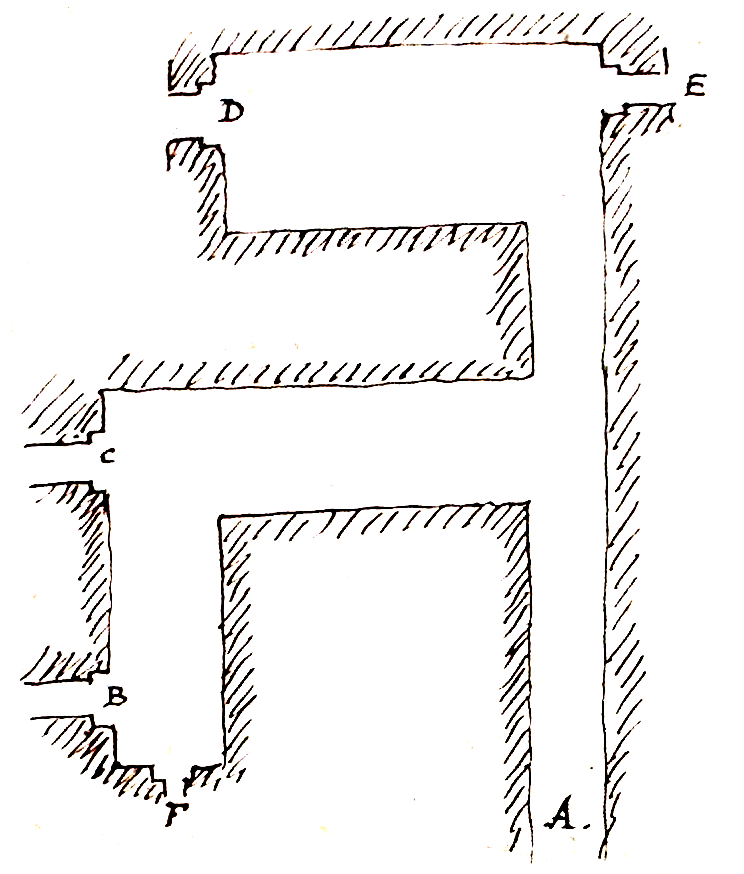
\includegraphics{CoEg_Mariette_1852-01-16_fig-1.png}
\end{center}
\indent Le plan incliné commence en A = B, C, D, E sont des portes qui\\
communiquent dans l’intérieur des souterrains à l’est par la porte B\\
que j’ai pénétrée le 12 novembre. F est une 5\textsuperscript{e} porte qui conduit\\
à des galeries inconnues, car elles sont ensablées jusqu’aux voutes [\textit{sic}].\\
{[rature]} Le plan incliné tout entier est, bien entendu, taillé dans\\
le roc. Or à hauteur d’appui sur chacune de ses parois, se\\
voient encore une quantité incroyable de stèles votives en\\
hiéroglyphes ou en démotiques. Le même fait se répète dans un\\
grand nombre de chambres de l’intérieur = Ce fait singulier\\
mérite, je crois, une grande attention et mon premier soin, à\\
la reprise des travaux, sera d’enlever toutes celles de ces stèles\\
que je pourrai rencontrer.\\
\indent J’ai encore bien des choses à vous dire. Mais, vous le voyez,\\
la place me manque. Ayez la complaisance de présenter mes hommages\\
à \gls{CoEg_abbr_00000001} de Rougé\gls{CoEg_pers_00000032}, à \gls{CoEg_abbr_00000001} de Longpérier\gls{CoEg_pers_00000033}, à \gls{CoEg_abbr_00000001} de Viel-Castel\gls{CoEg_pers_00000034}\\
et à \gls{CoEg_abbr_00000001} Villot\gls{CoEg_pers_00000035}. Si Dieu\gls{CoEg_pers_00000036} me conserve l’excellente santé dont je\\
jouis, je compte avoir encore ici du travail pour une année.\\
\indent Mais que de choses à faire.
\begin{center} \hspace{5cm} Votre tout dévoué serviteur :\\
\hspace{5cm} \gls{CoEg_abbr_00000002} Mariette\end{center}
\section*{Le 4 août 1852, d'Abousir, à [Nieuwerkerke]} \label{CoEg_Mariette_1852-08-04} \addcontentsline{toc}{section}{Le 4 août 1852, d'Abousir, à [Nieuwerkerke]}
{\footnotesize \noindent Institution et lieu de conservation : Archives nationales\gls{CoEg_org_00000024}, Pierrefitte-sur-Seine\\
Cote : \hyperref[CoEg_Mariette_ms_001]{20150497/118}, dossier 145 (Mariette, Auguste), lettre s. n.\\
Support : 1 feuille double.\\
Note : une copie non datée de cette lettre se trouve dans les papiers Mariette\gls{CoEg_pers_00000001} conservés au sein du fonds Maspero à la bibliothèque de l'Institut de France\gls{CoEg_org_00000004} (ms. 4061 (2), f\textsuperscript{os} 24-27 pour cette lettre), parmi la copie de douze de ses lettres dont la plupart sont issues de son dossier personnel de l'administration des musées nationaux (aujourd'hui aux Archives nationales\gls{CoEg_org_00000024} sous la cote \hyperref[CoEg_Mariette_ms_001]{20150497/118}, dossier 145), et de sept lettres envoyées par lui à Kabis\gls{CoEg_pers_imn} (aujourd'hui aux Archives nationales\gls{CoEg_org_00000024} aussi sous la cote AB/XIX/4195). Ces copies ne sont pas de la main de Mariette\gls{CoEg_pers_00000001}, mais correspondent à une écriture ancienne (parmi elles, la lettre la plus récente est de 1869) ; leur interprétation n'est d'ailleurs pas toujours très fiable.
\begin{center} {[1\textsuperscript{re} page, r\textsuperscript{o}]}\end{center}}
\begin{flushright} Du désert d’Abousyr\gls{CoEg_place_00000008}, le 4 août 1852.\end{flushright}

\hspace{1cm}Monsieur\gls{CoEg_pers_00000002},\\

\indent J’ai écrit avant-hier à \gls{CoEg_abbr_00000001} le Ministre de l’Intérieur\gls{CoEg_pers_00000037} pour l’avertir\\
du départ très-prochain d’Alexandrie\gls{CoEg_place_00000006} de trois de mes caisses. Ces\\
caisses seront vers le 15 août à Marseille\gls{CoEg_place_00000018}, et si le commissionnaire\footnote{La fin du mot est écrite par-dessus un autre mot illisible.}\\
de roulage de l’Intérieur\gls{CoEg_org_00000009} veut bien se hâter, vous les recevrez quelques\\
jours après.\\
\indent J’ai joint à ma lettre à \gls{CoEg_abbr_00000001} le Ministre\gls{CoEg_pers_00000037} [rature] une autre\\
lettre pour \gls{CoEg_abbr_00000009} B{[oujon ?]}\gls{CoEg_pers_00000038} et Verrier\gls{CoEg_pers_00000039}, 75, rue de Rambuteau, aujourd’hui\\
chargé des transports de votre Ministère\footnote{Mariette\gls{CoEg_pers_00000001} se réfère-t-il au ministère de l'Intérieur\gls{CoEg_org_00000009} ou au ministère d'État et de la maison de l'empereur\gls{CoEg_org_00000010} ? l'administration des musées nationaux (bientôt impériaux) et du Louvre était passée de la tutelle de celui-là à celui-ci entre décembre 1851 et février 1852.}. Ayez la bonté, Monsieur,\\
de faire dire à ce Monsieur l’intérêt que vous avez à posséder ces\\
caisses, et recommandez-leur surtout de ne les manier qu’avec\\
précautions, car les objets qu’ils contiennent, tout en pierre qu’ils\\
sont, sont des plus fragiles.\\
\indent Je prie aussi \gls{CoEg_abbr_00000001} le Ministre de l’Intérieur\gls{CoEg_pers_00000037} de vous faire passer\\
une copie de l’extrait de mon catalogue que je lui ai envoyé. Cet\\
extrait concerne les monuments renfermés dans les trois colis. Je\\
vous serait très-obligé si vous vouliez bien réclamer cette copie\\
aux Beaux-Arts\gls{CoEg_org_00000011}.\\
\indent J’aurais voulu joindre à cet envoi quelque monument qui, pour\\
son exécution artistique, vous intéressât plus particulièrement. Mais\\
les caisses sont trop lourdes, ou bien elles sont encore ici et vont\\
faire partie d’une seconde expédition pour Alexandrie\gls{CoEg_place_00000006}. Je tâcherai\\
néanmoins de vous faire passer un de ces jours mon \textit{écrivain\gls{CoEg_obj_00000008}}. Ce\\
monument est au moins de la IV\textsuperscript{e} dynastie et il surpasse, pour le\\
modelé des chairs et l’expression générale du personnage, tout ce\\
que vous avez vu jusqu’ici, même de ce qu’on appelle la bonne époque.\\
La photographie que je vous en ai envoyée a mal rendu ces formes si\\
naturelles, et vous ne devez pas la regarder comme une copie exacte du modèle.
{\footnotesize \begin{center} {[1\textsuperscript{re} page, v\textsuperscript{o}]}\end{center}}
\indent J’ai jusqu’ici livré au gouvernement égyptien\gls{CoEg_org_00000008} 656 monuments, et je\\
m’arrange de manière à passer pour n’en garder aucun par devers moi,\\
ce qui, entre nous, est tout de la contraire de la vérité. Son Altesse\gls{CoEg_pers_00000016} sera\\
enchantée quand elle apprendra mon empressement à obéir à ses\\
ordres et elle n’en sera que plus disposée à nous faire plus tard\\
un second cadeau. Mais pour cela je pense qu’il faudrait, dès-\\
-à-présent, que le nouveau consul-général\gls{CoEg_pers_00000040} d’Egypte\gls{CoEg_place_00000003} (de qui tout\\
dépend) fût instruit par le Ministre des Affaires Etrangères\gls{CoEg_pers_00000041} de l’importance\\
que le gouvernement français\gls{CoEg_org_00000012} attache aux fouilles du Sérapéum\gls{CoEg_place_00000004}, afin\\
qu’il ne soit plus, comme \gls{CoEg_abbr_00000001} Le Moyne\gls{CoEg_pers_00000024}, qu’on a laissé un an\\
sans instruction, exposé à pêcher {[\textit{sic}]} par ignorance. Causez-en avec\\
\gls{CoEg_abbr_00000001} Batissier\gls{CoEg_pers_00000027}, et celui-ci vous dira que si le nouveau Consul-\\
-général\gls{CoEg_pers_00000040} le veut bien, il peut obtenir de Son Altesse\gls{CoEg_pers_00000016} même le droit\\
de fouiller dans l’Egypte\gls{CoEg_place_00000003} entière, ce que je désire bien vivement,\\
Monsieur, car il m’en coûterait beaucoup de retourner en France\\
sans avoir visité Thèbes\gls{CoEg_place_00000019} et la Haute-Egypte\gls{CoEg_place_00000020}.\\
\indent \gls{CoEg_abbr_00000001} D’Anastasy\gls{CoEg_pers_00000015} est mort il y a quelques jours\footnote{Il s'agissait d'une fausse rumeur (voir la \hyperref[CoEg_Mariette_1852-09-04]{lettre du 4 septembre 1852}) ; D'Anastasi\gls{CoEg_pers_00000015} mourrut en 1860.} et peut-être\\
ses héritiers n’auront-ils pas la même prétention quant à la\\
collection de Livourne\gls{CoEg_place_00000012}. J’ai déjà écrit à Alexandrie\gls{CoEg_place_00000006} pour qu’on\\
sonde le terrain à ce sujet et je vous ferai part de toutes les\\
informations que je pourrai recueillir. De votre côté, dites-moi\\
si, avec une réduction considérable de prix, vous seriez disposé à\\
terminer cette affaire.\\
\indent Rien de nouveau ici. J’attends avec impatience le moment de\\
reprendre les travaux et les souterrains grecs m’empêchent de\\
dormir. Du reste, si on m’accorde des fonds, je pousserai les fouilles\\
avec la plus grande activité, car j’ai hâte d’en finir. En six mois\\
j’espère que tout sera fait.
{\footnotesize \begin{center} {[2\textsuperscript{e} page, r\textsuperscript{o}]}\end{center}}
\indent Mais le plus difficile sera d’emballer les grands lions grecs\\
et les autres statues de même style. Ces objets ont été taillés dans\\
une pierre très-friable qui s’écaille et je ne vois pas de moyen de\\
les ramener sans les briser. Aussi, Monsieur, je m’adresse à vous\\
et je vous prie de me faire savoir si vous ne connaissez pas\\
quelque composition chimique qui rende à la pierre sa dureté\\
primitive.\footnote{En juillet 1851, Rochas publia dans les comptes rendus de l'Académie des sciences une lettre sur le procédé de silicatisation ; il mentionnait un voyage en Orient au cours duquel il avait observé les monuments du Sérapéum et échangé avec Mariette à ce sujet ; le département égyptien du Louvre constitua d'ailleurs en 1853 un dossier à ce sujet - conservé sous la cote 20144775/24 aux Archives nationales. Rochas obtint l'autorisation de faire des essais de son procédé sur des statues égyptiennes du Louvre (voir aussi l'article 20144793/33 des Archives nationales où se trouvent des courriers archivés par le département des sculptures).} Dans ce cas, veuillez me la faire connaître, afin que\\
je l’applique ici, car les monuments dont je vous entretiens, sans\\
être très-précieux au point de vue de l’art, le sont beaucoup\\
pour les archéologues, et dans tous les cas feront toujours au\\
Louvre\gls{CoEg_org_00000002} un excellent fond de salle. En attendant que vous veuillez\\
bien me répondre, ces monuments sont sous le sable à l’abri de\\
toute cause de destruction.\\
\indent Je ne compte pas vous envoyer toutes les statues grecques de\\
l’hémicycle de l’Apéum. Elles sont trop mauvaises. J’en ferai\\
un choix d’une ou deux. Mais je vous demanderai à mouler\\
les autres à cause des inscriptions grecques qu’on y lit.\\
\indent Vous aurez remarqué sans doute dans mon plan général\\
de la tombe d’Apis\gls{CoEg_pers_00000011} et d’Osiris\gls{CoEg_pers_00000042} l’indication, dans la tombe\\
d’Osiris\gls{CoEg_pers_00000042}, de quelques salles éboulées. J’ai oublié de noter, dans\\
mon programme des travaux qui restent à faire, le déblaiement\\
de ces salles. Je les ai bien nettoyées jusqu’à un mètre du sol,\\
mais pas assez pour être sûr qu’ils n’y reste rien. Il existe là\\
en effet d’énorme rochers qui recouvrent peut-être des monuments\\
précieux et que j’ai craint de faire sauter. Je crois bien que\footnote{Mariette\gls{CoEg_pers_00000001} avait écrit \og ~qu'~\fg, mais a biffé l'apostrophe et complété en \og ~que~\fg.} des\\
fouilles plus attentives dans cette partie du Sérapéum\gls{CoEg_place_00000004} pourront\\
ne pas être improductives.
{\footnotesize \begin{center} {[2\textsuperscript{e} page, v\textsuperscript{o}]}\end{center}}
\indent J’ai à vous remercier beaucoup, Monsieur, à vous remercier du\\
fond de mon cœur de ce que vous avez bien voulu [pour ma femme\gls{CoEg_pers_00000005} ?]\footnote{Si \og ~ma~\fg est assez clair, le premier mot pourrait se lire \og ~fait~\fg.}.\\
Vous savez bien que mon dévouement et celui de toute ma famille\\
vous est acquis et je n’ai pas besoin de vous exprimer par de\\
plus longues phrases un sentiment que vous savez sincère. Je suis\\
tout entier à vos ordres et prêt pour vous à aller, si vous le voulez,\\
au bout du monde.\\
\indent Hier j’ai fait cuire des œufs sous le sable. Le soleil nous dévore\\
et le sable est si chaud qu’on ne peut littéralement en tenir une\\
poignée dans la main. Heureusement nous touchons au terme\\
de ces chaleurs accablantes. Le Nil\gls{CoEg_place_00000021} monte et couvre déjà les\\
campagnes ; la fraîcheur vient avec lui. Quel beau pays que\\
l’Egypte\gls{CoEg_place_00000003} et comme le temps des\footnote{Le mot a été inscrit sur d'autres lettres.} Ramsès reviendrait pour lui\\
s’il était à la France\gls{CoEg_place_00000016}. En attendant les Anglais le convoitent\\
bien et ne tarderont pas à en faire leur Algérie\gls{CoEg_place_00000022}. Adieu alors\\
les antiquités pour le Louvre\gls{CoEg_org_00000002}, adieu le Sérapéum\gls{CoEg_place_00000004} que le sable\\
recouvre encore.\\
\indent Présentez, s’il vous plaît, mes civilités à \gls{CoEg_abbr_00000001} de Viel-Castel\gls{CoEg_pers_00000034},\\
à \gls{CoEg_abbr_00000001} de Longpérier\gls{CoEg_pers_00000033}, à \gls{CoEg_abbr_00000001}\\
Villot\gls{CoEg_pers_00000035}, à \gls{CoEg_abbr_00000001} {[A[n/u]g[n/u]iot ?]}\gls{CoEg_pers_00000043}, à \gls{CoEg_abbr_00000001} {[Lauzay/Sanzay ?]}\gls{CoEg_pers_00000044},\\
et à bien d’autres que j’oublie sans doute, car depuis bientôt\\
deux ans j’ai eu le temps de laisser une pauvre mémoire s’envoler\\
avec le vent du désert. Quant à vous, Monsieur, je n’ai pas\\
besoin de vous renouveler l’assurance de tous mes sentiments\\
de respect. Vous savez que je suis tout à vous
\begin{center} \hspace{5cm}\gls{CoEg_abbr_00000002} Mariette\end{center}
Je vous fais mes excuses pour une bien mauvaise petite boîte qui s’est\\
glissée dans le colis qui vous a été apportée par Batissier\gls{CoEg_pers_00000027}. Cette petite\\
boîte ne contenait que du rebut, et elle a été envoyée par erreur au\\
Caire\gls{CoEg_place_00000010}.\\
\indent Faites-moi le plaisir de bien remercier pour moi Batissier\gls{CoEg_pers_00000027} de tous\\
les services qu’il m’a rendu au Caire\gls{CoEg_place_00000010}. Dieu\gls{CoEg_pers_00000036} veuille que je revoie bientôt cet excellent
\begin{flushright}ami.\end{flushright}
\section*{Le 20 août 1852, d'Abousir, au ministre de l'Intérieur} \label{CoEg_Mariette_1852-08-20} \addcontentsline{toc}{section}{Le 20 août 1852, d'Abousir, au ministre de l'Intérieur}
{\footnotesize \noindent Institution et lieu de conservation : Archives nationales\gls{CoEg_org_00000024}, Pierrefitte-sur-Seine\\
Cote : \hyperref[CoEg_Mariette_ms_001]{20150497/118}, dossier 145 (Mariette, Auguste), lettre s. n.\\
Support : 1 feuille double.\\
Note : une copie non datée de cette lettre se trouve dans les papiers Mariette\gls{CoEg_pers_00000001} conservés au sein du fonds Maspero à la bibliothèque de l'Institut de France\gls{CoEg_org_00000004} (ms. 4061 (2), f\textsuperscript{os} 28-29 pour cette lettre), parmi la copie de douze de ses lettres dont la plupart sont issues de son dossier personnel de l'administration des musées nationaux (aujourd'hui aux Archives nationales\gls{CoEg_org_00000024} sous la cote \hyperref[CoEg_Mariette_ms_001]{20150497/118}, dossier 145), et de sept lettres envoyées par lui à Kabis\gls{CoEg_pers_imn} (aujourd'hui aux Archives nationales\gls{CoEg_org_00000024} aussi sous la cote AB/XIX/4195). Ces copies ne sont pas de la main de Mariette\gls{CoEg_pers_00000001}, mais correspondent à une écriture ancienne (parmi elles, la lettre la plus récente est de 1869) ; leur interprétation n'est d'ailleurs pas toujours très fiable.}
\begin{center} {\footnotesize[1\textsuperscript{re} page, r\textsuperscript{o}]}\\
Du désert d’Abousyr\gls{CoEg_place_00000008}, le 20 août 1852.\end{center}
\indent A Monsieur\\
\begin{center}Monsieur le Ministre Secrétaire d’État au département\end{center}
\begin{flushright}de l’Intérieur\gls{CoEg_org_00000009}, à Paris\gls{CoEg_place_00000002}.\end{flushright}

\hspace{1cm} Monsieur le Ministre\gls{CoEg_pers_00000037},\\

\indent Par ma lettre en date du 1\textsuperscript{er} Août dernier, j’ai eu l’honneur\\
de vous faire savoir que je venais de m’entendre avec \gls{CoEg_abbr_00000001} le Consul-\\
Général\gls{CoEg_pers_00000024} de France\gls{CoEg_place_00000016} à Alexandrie\gls{CoEg_place_00000006} à l’effet d’expédier, à destination\\
de Marseille\gls{CoEg_place_00000018}, trois colis d’antiquités provenant du Sérapéum\gls{CoEg_place_00000004}\\
de Memphis\gls{CoEg_place_00000005}. – J’avais alors entre les mains une lettre de \gls{CoEg_abbr_00000001} le\\
second \gls{CoEg_term_00000006}\gls{CoEg_pers_imn} du Consulat-Général\gls{CoEg_org_00000006} qui m’autorisait à vous\\
faire cette déclaration, et d’un autre côté je savais officieusement\\
notre honorable consul-général\gls{CoEg_pers_00000024} tout disposé à seconder mes intentions\\
à l’égard du transport de ces mêmes colis.\\
\indent Mais à l’époque où nous décidions ensemble cette mesure,\\
le vapeur qui devait être chargé du transport n’était pas encore\\
à Alexandrie\gls{CoEg_place_00000006} et nous ne devions pas supposer qu’un empêchement\\
quelconque pût se présenter. C’est pourtant ce qui advint et il\\
résulte de la copie de la lettre de \gls{CoEg_abbr_00000001} Le Moyne\gls{CoEg_pers_00000024} jointe ici\footnote{La lettre en question est recopiée par Mariette\gls{CoEg_pers_00000001} à la main sur la deuxième page de la feuille, en-tête compris.} qu’à\\
son arrivée à Alexandrie\gls{CoEg_place_00000006} le capitaine du bâtiment, consulté\\
à ce sujet, déclara ne pouvoir se charger de l’embarquement
\begin{flushright}de trois\end{flushright}
{\footnotesize \begin{center} {[1\textsuperscript{re} page, v\textsuperscript{o}]}\end{center}}
de trois caisses. J’ai donc à vous prier aujourd’hui de regarder comme\\
non avenue ma lettre du 1\textsuperscript{er} Août ; les antiquités que j’eusse\\
désiré expédier en France\gls{CoEg_place_00000016} le plus promptement possible attendront\\
avec les autres dans les magasins du Consulat-Général\gls{CoEg_org_00000006} le\\
navire de guerre que je vous supplie de nouveau de vouloir\\
bien nous faire envoyer.\\
\indent D’ailleurs, Monsieur le Ministre, vous voudrez bien\\
considérer que la fausse démarche que j’ai faite le 1\textsuperscript{er} août\\
était inévitable, tant par la nécessité où je me trouvais de\\
vous informer de la résolution prise, que par la distance qui\\
me sépare d’Alexandrie\gls{CoEg_place_00000006} et l’arrivée tardive du bateau-poste\\
dans le port de cette ville. La lettre de \gls{CoEg_abbr_00000001} le Consul-Général\gls{CoEg_pers_00000024}\\
porte en effet la date du 4 août ; elle m’est ainsi arrivée\\
le 7, c’est-à-dire le jour même du départ du paquebot qui\\
qui emportait ma lettre d’avis. Je ne crois donc pas qu’il y ait\\
de ma faute si la nouvelle que je me suis hâté de porter à\\
votre connaissance a pu exposer vos bureaux à des démarches\\
inutiles.\\
\indent J’ai l’honneur d’être avec le plus profond respect,
\begin{center} Monsieur le Ministre,\end{center}
\begin{center}\hspace{5cm} Votre très-humble\\
\hspace{5cm} et très-obéissant serviteur.\\
\hspace{5cm} \gls{CoEg_abbr_00000002} Mariette\end{center}
{\footnotesize \begin{center} {[2\textsuperscript{e} page, r\textsuperscript{o}]}\end{center}}
Copie.\\
Agence et Consulat Général\gls{CoEg_org_00000006}\\
\hspace{3cm} de France\gls{CoEg_place_00000016}\\
\hspace{3cm} en Egypte\gls{CoEg_place_00000003}.
\begin{flushright}Alexandrie\gls{CoEg_place_00000006}, le 4 avril 1852.\end{flushright}
\begin{flushright}Monsieur \gls{CoEg_abbr_00000002} Mariette\gls{CoEg_pers_00000001}, à Abousyr\gls{CoEg_place_00000008}.\end{flushright}

\hspace{1cm} Monsieur,\\

\indent D’après la lettre que vous m’avez fait l’honneur de m’écrire le 29\\
du mois dernier, j’ai prié \gls{CoEg_abbr_00000001} le Commandant du paquebot français qui\\
se trouve actuellement dans le port d’Alexandrie\gls{CoEg_place_00000006} de venir voir les trois\\
caisses que vous désirez faire parvenir aussi promptement que possible\\
en France\gls{CoEg_place_00000016} ; mais ce commandant, après les avoir examinées, m’a\\
dit qu’il n’avait pas à son bord d’appareil assez fort pour soulever\\
et embarquer notamment la caisse \gls{CoEg_abbr_00000010} 40, en un mot, qu’il ne\\
pouvait pas se charger de la prendre à cause de son poids et de\\
sa grandeur ; dans cet état de choses, j’ai pensé qu’il y avait d’autant\\
moins d’inconvénients à suspendre l’envoi des deux autres caisses\\
\gls{CoEg_abbr_00000011} 4 et 7 que, sans doute, un bâtiment de l’État\gls{CoEg_org_00000012} ne devra plus\\
beaucoup tarder maintenant à venir chercher tous vos monuments.\\
Du reste lorsqu’il s’agira de leur départ, je me chargerai volontiers\\
de les adresser à \gls{CoEg_abbr_00000001} l’Agent du Ministère des Affaires Etrangères\gls{CoEg_org_00000007}\\
à Marseille\gls{CoEg_place_00000018} pour les consigner à \gls{CoEg_abbr_00000001} \gls{CoEg_abbr_00000012} Pastré\gls{CoEg_pers_00000046} ....\\
\indent Agréez, Monsieur – etc.
\begin{center} \hspace{5cm} Signé A. Le Moyne \gls{CoEg_pers_00000024}.\end{center}
\section*{Le 3 septembre 1852, d'Abousir, au ministre de l'Intérieur} \label{CoEg_Mariette_1852-09-03} \addcontentsline{toc}{section}{Le 3 septembre 1852, d'Abousir, au ministre de l'Intérieur}
{\footnotesize \noindent Institution et lieu de conservation : Archives nationales\gls{CoEg_org_00000024}, Pierrefitte-sur-Seine\\
Cote : \hyperref[CoEg_Mariette_ms_001]{20150497/118}, dossier 145 (Mariette, Auguste), lettre s. n.\\
Support : 1 feuille double.\\
Note : une copie non datée de cette lettre se trouve dans les papiers Mariette\gls{CoEg_pers_00000001} conservés au sein du fonds Maspero à la bibliothèque de l'Institut de France\gls{CoEg_org_00000004} (ms. 4061 (2), f\textsuperscript{os} 30-33 pour cette lettre), parmi la copie de douze de ses lettres dont la plupart sont issues de son dossier personnel de l'administration des musées nationaux (aujourd'hui aux Archives nationales\gls{CoEg_org_00000024} sous la cote \hyperref[CoEg_Mariette_ms_001]{20150497/118}, dossier 145), et de sept lettres envoyées par lui à Kabis\gls{CoEg_pers_imn} (aujourd'hui aux Archives nationales\gls{CoEg_org_00000024} aussi sous la cote AB/XIX/4195). Ces copies ne sont pas de la main de Mariette\gls{CoEg_pers_00000001}, mais correspondent à une écriture ancienne (parmi elles, la lettre la plus récente est de 1869) ; leur interprétation n'est d'ailleurs pas toujours très fiable.
\begin{center} {[1\textsuperscript{re} page, r\textsuperscript{o}]}\end{center}}
\noindent lettres de \gls{CoEg_abbr_00000001}\\
Mariette\gls{CoEg_pers_00000001}\footnote{Annotation au crayon rouge.}\\

\noindent A classer\footnote{Annotation au crayon gris.}\\
\begin{flushright} Du désert d’Abousyr\gls{CoEg_place_00000008}, le 3 septembre 1852.\end{flushright}
\indent A Monsieur\\
\begin{center}Monsieur le Ministre Secrétaire d’Etat au Département\\
de l’Intérieur\gls{CoEg_org_00000009}\end{center}
\begin{flushright}à Paris\gls{CoEg_place_00000002}.\end{flushright}

\hspace{1cm}Monsieur le Ministre\gls{CoEg_pers_00000037},\\

\indent J’ai déjà eu souvent de vous entretenir de la position\\
difficile qui résulte pour moi des conventions arrêtées au mois de février\\
dernier entre le \gls{CoEg_term_00000002}\gls{CoEg_pers_00000016} d’Egypte\gls{CoEg_place_00000003} et le gouvernement français\gls{CoEg_org_00000012}. En vertu de\\
ces conventions, mon droit de fouiller ne s’étend pas au-delà du Sérapéum\gls{CoEg_place_00000004}\\
de Memphis\gls{CoEg_place_00000005} et chacun des objets découverts appartient de droit au gouvernement\\
égyptien\gls{CoEg_org_00000008} qui s'en empare aussitôt trouvés et les fait transporter à la Citadelle\gls{CoEg_place_00000023}\\
du Caire\gls{CoEg_place_00000010}. Deux officiers d’état-major de l’armée égyptienne\gls{CoEg_org_00000013} stationnent\\
continuellement sur les lieux, enregistrent jour par jour les résultats obtenus\\
et veillent à ce que rien ne soit détourné. C’est ainsi que, depuis le\\
mois de février jusqu’au mois de juin, j’ai été forcé de livrer à ces agents\\
656 objets antiques.\\
\indent Je viens de vous dire que ces conventions me faisaient une position\\
très-difficile. En effet, d’une part, je ne crois pas devoir vous cacher mon\\
désir d’aller visiter, après l’achèvement des travaux du Sérapéum\gls{CoEg_place_00000004}, les ruines\\
de la Haute-Egypte\gls{CoEg_place_00000020} que je n’ai jamais vues et que, pour moi qui fais\\
profession d’égyptologie, il serait trop dur de ne jamais voir après les avoir\\
approchées de si près ; or un voyage de cette sorte, entrepris en érudit plutôt\\
qu’en touriste, exige toujours quelques petites déblaiements, puisque la plupart\\
des inscriptions de l’Egypte\gls{CoEg_place_00000003} ne peuvent être copiées et étudiées qu’à condition\\
d’écarter le sable qui les couvre, ce qui, depuis près d’une année, est formellement\\
interdit à tous les voyageurs. D’autre part je suis obligé de vous rappeler\\
que les circonstances me forcent à violer ces mêmes conventions arrêtées entre\\
\begin{flushright}les deux\end{flushright}
 {\footnotesize \begin{center} {[1\textsuperscript{re} page, v\textsuperscript{o}]}\end{center}}
les deux gouvernements et que loin de livrer au \gls{CoEg_term_00000002}\gls{CoEg_pers_00000016} les monuments découverts\\
je lui laisse ceux de ces objets qui me semblent n’avoir aucune valeur, et que\\
j’organise pour les autre un système de contrebande qu’à cause même de sa\\
hardiesse je crains toujours de voir s’écrouler. C’est là, Monsieur le Ministre,\\
ce qui me fait la situation dont je me plains, situation sur laquelle\\
j’appelle toute votre attention, parce qu’elle est très-délicate et en même\\
temps très-périlleuse.\\
\indent Je viens donc vous prier de vouloir bien, dans le cas où vous\\
adopteriez ces vues, vous avec \gls{CoEg_abbr_00000001} le Ministre des Affaires Etrangères\gls{CoEg_pers_00000041} et\\
faire donner au nouveau Consul-Général\gls{CoEg_pers_00000040} de France\gls{CoEg_place_00000016} en Egypte\gls{CoEg_place_00000003} des instructions\\
au nom desquelles cet agent pourrait travailler à faire obtenir, en ce qui\\
me concerne, des conditions un peu plus libérales. Je crois devoir vous faire\\
observer à ce sujet que ce que j’ai l’honneur de vous proposer me paraît d’autant\\
moins dangereux à solliciter du Vice-Roi\gls{CoEg_pers_00000016} que le gouvernement français\gls{CoEg_org_00000012}, en\\
m’envoyant l’ordre exprès de livrer les objets découverts, a reconnu par là\\
même le droit de \gls{CoEg_abbr_00000003}\gls{CoEg_pers_00000016} et a donné en même temps la preuve de son désir\\
d’entretenir avec elle des relations amicales. Les 656 objets que j’ai livrés me\\
paraissent ainsi un argument en notre faveur. – D’un autre côté, peut-être\\
les conditions dans lesquelles nous nous trouvons aujourd’hui ne sont-elles\\
plus les mêmes qu’au mois de février dernier. Mes travaux, vous vous le\\
rappelez, étaient suspendus depuis le 21 novembre, et le 12 septembre auparavant\\
l’ordre m’avait été donné, de la part du Vice-Roi\gls{CoEg_pers_00000016}, de livrer tous les\\
monuments que j’avais en magasin. Mais le Vice-Roi\gls{CoEg_pers_00000016} n’était, en quelque\\
sorte, pour rien dans cette affaire ; il était poussé aux mesures un peu\\
violentes dont je fus alors l’objet par son conseiller ordinaire, \gls{CoEg_abbr_00000001} le\\
Consul-Général anglais\gls{CoEg_pers_00000018}. C’est n’est pas en effet que le \gls{CoEg_term_00000002}\gls{CoEg_pers_00000016} attache un\\
grand prix aux antiquités qui couvrent son royaume et qu’il ait regardé\\
mes découvertes comme une spoliation de son propre bien : vous savez au\\
contraire avec quelle désolante persévérance ses agents détruisent un à un\\
les vénérables témoins de la grandeur des Pharaons. Ce n’est pas non plus\\
qu’il eût eu sérieusement l’idée, ou de s’approprier mes monuments, ou de\\
m’empêcher de continuer mes travaux ; je crois que si nous avions résolument\\
cédé devant des exigences, en réservant notre recours à l’opinion publique,\\
{\footnotesize \begin{center} {[2\textsuperscript{e} page, r\textsuperscript{o}]}\end{center}}
\noindent nous eussions été moins embarrassés de notre défaite que \gls{CoEg_abbr_00000001} Murray\gls{CoEg_pers_00000018} et lui\\
d’une victoire qu’ils ne cherchaient pas, qu’ils ne désiraient pas, parce que\\
le droit seul \textsuperscript{qu’ils invoquaient} ne suffisait pas pour prendre violemment possession des monuments\\
acquis avec l’argent de la France\gls{CoEg_place_00000016} et l’autorisation régulière du \gls{CoEg_term_00000002}\gls{CoEg_pers_00000016}\\
lui-même. Ce qu’on voulait au contraire, c’était que par nos fautes nous\\
créassions un droit nous même un droit nouveau à \gls{CoEg_abbr_00000003}\gls{CoEg_pers_00000016}, et pour cela\\
on a affecté de traiter directement avec moi sans passer par l’intermédiaire\\
obligé du Consul-Général\gls{CoEg_pers_00000024}, afin de profiter de mon inexpérience et de faire\\
naître par ma propre incapacité une raison légitime de garder les monuments\\
confisqués et de m’interdire l’accès du Sérapéum\gls{CoEg_place_00000004}. Deux mois après, les\\
Anglais se fussent installés sur les ruines que, selon eux, nous n’eussions\\
pas su garder et les 515 monuments confisqués eussent bientôt après avoir pris\\
incognito le chemin de Londres\gls{CoEg_place_00000011} avec ceux que la continuation des fouilles\\
eût fait découvrir. Je vous répète donc, Monsieur le Ministre, que tout cela\\
a été le résultat d’une intrigue anglaise ; mais j’ajoute que peut-être\\
aujourd’hui les réclamations de notre consul-général\gls{CoEg_pers_00000040} ne trouveraient pas\\
\gls{CoEg_abbr_00000003}\gls{CoEg_pers_00000016} dans les mêmes dispositions.\\
\indent En tout cas, \gls{CoEg_abbr_00000001} Sabatier\gls{CoEg_pers_00000040} pourra sans doute à son arrivée\\
sonder le terrain et je pense, Monsieur le Ministre, que si le moment venait\\
où ce fonctionnaire croirait pouvoir risquer la demande que j’ai l’honneur\\
de vous soumettre, il devrait d’autant mieux saisir l’occasion que le\\
changement tout récent de \Gls{CoEg_term_00000004} de la province de Gyzeh\gls{CoEg_place_00000007} va amener\\
un mouvement dans le personnel de mes officier et que je ne sais pas s’il\\
me sera toujours possible d’échapper à la surveillance de ces gens et de\\
sauver au profit du Louvre\gls{CoEg_org_00000002} les monuments nouveaux que la reprise des\\
travaux pourra me faire découvrir.\\
\indent J’ai l’honneur d’être avec le plus profond respect,
\begin{center}Monsieur le Ministre,\end{center}
\begin{center}\hspace{5cm}Votre très-humble\\
\hspace{5cm}et très-obéissant serviteur.\\
\hspace{5cm}\gls{CoEg_abbr_00000002} Mariette\end{center}
{\footnotesize\begin{center} {[2\textsuperscript{e} page, v\textsuperscript{o}]}\end{center}}
\noindent \gls{CoEg_abbr_00000008} Après avoir rappelé au commencement de cette lettre les conditions qui nous sont imposées par le\\
gouvernement\gls{CoEg_org_00000008} du \gls{CoEg_term_00000002}\gls{CoEg_pers_00000016}, je crois devoir vous faire connaître celles que, dans les mêmes circonstances,\\
le Vice-Roi\gls{CoEg_pers_00000016} a consenties en faveur du gouvernement anglais\gls{CoEg_org_00000014}. Il y a un an environ, la Société Géologique\gls{CoEg_org_00000015}\\
de Londres\gls{CoEg_place_00000011} manifesta le désir de faire quelques excavations sur le sol des anciennes capitales de\\
l’Egypte\gls{CoEg_place_00000003}. L’enceinte d’Héliopolis\gls{CoEg_place_00000024} fut explorée l’été passé, et la saison actuelle a été occupée par\\
de grandes fouilles sur l’emplacement de Memphis\gls{CoEg_place_00000005}. Mais, ainsi que j’ai pu m’en assurer par\\
des visites presque quotidiennes, la géologie n’est, à Memphis\gls{CoEg_place_00000005} du moins, que l’accessoire de\\
l’archéologie, et c’est le Musée Britannique\gls{CoEg_org_00000005} qui, surtout, profitera de ces travaux. En effet de\\
longues tranchées ont été ouvertes autour du colosse de Ramsès II\gls{CoEg_pers_00000026} à Myt-Rahyneh\gls{CoEg_place_00000025} et poussées\\
dans toutes les directions à travers les buttes de décombres qui recouvrent Memphis\gls{CoEg_place_00000005}. Chacune\\
de ces buttes a été ouverte, et en ce moment même les travailleurs de la Société\gls{CoEg_org_00000015}, chassés des\\
terres cultivées par l’inondation, viennent s’installer au milieu des sables de la nécropole\\
avec lesquels la géologie ne peut avoir rien à faire. Ces recherches, poursuivies avec\\
persévérance depuis cinq mois, n’ont pas été vaines ; l’emplacement et les limites du temple\\
de Ptah\gls{CoEg_pers_00000047} sont reconnus, les restes d’un nombre incroyable de colosses en granit sont retrouvés,\\
et le British Muséum\gls{CoEg_org_00000005} va s’enrichir d’une cinquantaine de statuettes de toute matière,\\
débris de l’ancienne splendeur du fameux temple de Vulcain\gls{CoEg_pers_00000047}. – Or ces recherches\\
se font toutes exclusivement aux frais du gouvernement égyptien\gls{CoEg_org_00000008}. Aussitôt que l’intention\\
de la Société Géologique\gls{CoEg_org_00000015} a été connue, \gls{CoEg_abbr_00000003}\gls{CoEg_pers_00000016} s’est empressée de mettre à la disposition de\\
\gls{CoEg_abbr_00000001} Murray\gls{CoEg_pers_00000018}, outre \gls{CoEg_abbr_00000004} Hékékyan-\gls{CoEg_term_00000003}\gls{CoEg_pers_00000048} comme directeur, un capitaine d’état-major comme\\
surveillant-général, trois ingénieurs détachés pour ce service du \gls{CoEg_term_00000007} des Travaux Publics\gls{CoEg_org_00000016},\\
et des ouvriers en aussi grand nombre qu’il pourrait en désirer. Le traitement de ces\\
agents et des hommes à leurs ordres constitue, avec les frais d’approvisionnement, de\\
campement, de machines, d’outils etc. – une dépense de près de 6 000 \gls{CoEg_abbr_00000013} par mois que le\\
\gls{CoEg_term_00000002}\gls{CoEg_pers_00000016} supporte en faveur de l’Angleterre\gls{CoEg_place_00000015}. Ajoutez que, loin de contester à \gls{CoEg_abbr_00000001} Murray\gls{CoEg_pers_00000018}\\
le droit de posséder les antiquités provenant de ces fouilles, \gls{CoEg_abbr_00000003}\gls{CoEg_pers_00000016} fait les frais de leur transport\\
jusqu’à Alexandrie\gls{CoEg_place_00000006}. Enfin Hékékyan-\gls{CoEg_term_00000003}\gls{CoEg_pers_00000048} devant incessamment porter ses recherches sur\\
Abydos\gls{CoEg_place_00000026} et Thèbes\gls{CoEg_place_00000019}, le gouvernement égyptien\gls{CoEg_org_00000008} met à sa disposition un bâteau {[\textit{sic}]} à vapeur.\\
– Tels sont, Monsieur le Ministre, les avantages faits en cette circonstance à l’Angleterre\gls{CoEg_place_00000015}.\\
Je n’établis pas ce parallèle parce que je désire jouir des mêmes facilités que Hékékyan-\\
-\gls{CoEg_term_00000003}\gls{CoEg_pers_00000048}, et je ne crois pas non plus que la France\gls{CoEg_place_00000016} se soucie beaucoup de la collaboration\\
d’Abbas-\Gls{CoEg_term_00000002}\gls{CoEg_pers_00000016}. Ce que je demande, c’est que le gouvernement égyptien\gls{CoEg_org_00000008} ne mette\\
pas d’empêchement à mes travaux ; c’est aussi que – maintenant que nous avons\\
suffisamment reconnu le droit de \gls{CoEg_abbr_00000003}\gls{CoEg_pers_00000016} en lui livrant 656 objets – Le Vice-Roi\gls{CoEg_pers_00000016}\\
veuille bien, en étendant mon \gls{CoEg_term_00000005} à toute l’Egypte\gls{CoEg_place_00000003}, me permettre de disposer\\
des objets que j’aurai découverts. –
\section*{Le 4 septembre 1852, d'Abousir, à [Nieuwerkerke]} \label{CoEg_Mariette_1852-09-04} \addcontentsline{toc}{section}{Le 4 septembre 1852, d'Abousir, à [Nieuwerkerke]}
{\footnotesize \noindent Institution et lieu de conservation : Archives nationales\gls{CoEg_org_00000024}, Pierrefitte-sur-Seine\\
Cote : \hyperref[CoEg_Mariette_ms_001]{20150497/118}, dossier 145 (Mariette, Auguste), lettre s. n.\\
Support : 1 feuille double.\\
Note : une copie non datée de cette lettre se trouve dans les papiers Mariette\gls{CoEg_pers_00000001} conservés au sein du fonds Maspero à la bibliothèque de l'Institut de France\gls{CoEg_org_00000004} (ms. 4061 (2), f\textsuperscript{os} 34-35 pour cette lettre), parmi la copie de douze de ses lettres dont la plupart sont issues de son dossier personnel de l'administration des musées nationaux (aujourd'hui aux Archives nationales\gls{CoEg_org_00000024} sous la cote \hyperref[CoEg_Mariette_ms_001]{20150497/118}, dossier 145), et de sept lettres envoyées par lui à Kabis\gls{CoEg_pers_imn} (aujourd'hui aux Archives nationales\gls{CoEg_org_00000024} aussi sous la cote AB/XIX/4195). Ces copies ne sont pas de la main de Mariette\gls{CoEg_pers_00000001}, mais correspondent à une écriture ancienne (parmi elles, la lettre la plus récente est de 1869) ; leur interprétation n'est d'ailleurs pas toujours très fiable.
\begin{center} {[1\textsuperscript{re} page, r\textsuperscript{o}]}\end{center}}
\begin{flushright}Abousyr\gls{CoEg_place_00000008}, le 4 septembre 1852.\end{flushright}

\hspace{1cm} Monsieur\gls{CoEg_pers_00000002},\\

\indent Ayez la bonté de faire remettre à la\\
Direction des Beaux-Arts\gls{CoEg_org_00000011} les deux plis\\
ci-joints. Comme je désire que leur contenu\\
ne soit pas ignoré de vous, je devrais, ou vous\\
en envoyer un duplicata, ou les rédiger pour\\
vous-mêmes à votre propre adresse. Mais à\\
force d’attendre le courrier de France\gls{CoEg_place_00000016} qui\\
est pourtant arrivé à Alexandrie\gls{CoEg_place_00000006} le 31 du\\
mois dernier, je me trouve acculé à la\\
dernière heure du courrier qui part, et\\
le temps me manque. Veuillez donc prendre\\
connaissance de ces deux lettres, les cacheter,\\
et les envoyer au Ministre\gls{CoEg_pers_00000037} [rature] – . Je serais\\
très-aise, dans le cas où vous approuveriez\\
la demande qui fait l’objet de l’une de\\
ces lettres, que vous voulussiez bien l’appuyer\\
de votre influence.\\
\indent Comme je viens de vous le dire, le\\
courrier ne m’a rien apporté, et il me faut
{\footnotesize \begin{center} {[1\textsuperscript{re} page, v\textsuperscript{o}]}\end{center}}
\noindent remettre à 10 jours le plaisir d’avoir de\\
vos nouvelles. Il me tarde pourtant bien\\
de reprendre les travaux. Heureusement cela\\
ne peut plus tarder et permettez-moi de\\
vous dire que je compte surtout sur vous.\\
\indent Dans le cas où le Ministère\gls{CoEg_org_00000009} aurait\\
de l’argent à m’envoyer, priez \gls{CoEg_abbr_00000001} Fleury\\
Hérard\gls{CoEg_pers_00000049} de me permettre de tirer à vue\\
sur lui, au lieu de me remettre des lettres\\
de crédit sur \gls{CoEg_abbr_00000001} Aïdi\gls{CoEg_pers_00000050}. Quoique celui-ci\\
me fasse ses paiements en pièces de 5 \glspl{CoEg_term_00000008},\\
qui sont la monnaie principale du\\
pays, il \sout{veut} s’obstine à convertir\\
toujours les \glspl{CoEg_term_00000008} en piastres et à me\\
payer ces piastres en pièces de cinq\\
francs. Il en résulte un tripotage\\
auquel je n’entends rien. D’un autre\\
côté un négociant du Caire\gls{CoEg_place_00000010}, qui m’est\\
recommandé spécialement par \gls{CoEg_abbr_00000001} Le Moyne\gls{CoEg_pers_00000024},\\
m’offre de me solder en francs, comme\\
si nous étions à Paris\gls{CoEg_place_00000002}. J’aime mille\\
fois mieux cette offre vraisemblable qui\\
me permet de voir clair dans mes
{\footnotesize \begin{center} {[2\textsuperscript{e} page, v\textsuperscript{o}]}\end{center}}
\noindent comptes, et je voudrais pouvoir l’accepter.\\
J’écrirais à \gls{CoEg_abbr_00000001} Fleury Hérard\gls{CoEg_pers_00000049}, si peut-être\\
il n’était déjà trop tard. Dans tous les cas,\\
si vous veniez à le rencontrer, ayez la bonté\\
de l’entretenir de cette affaire sur laquelle\\
d’ailleurs Batissier\gls{CoEg_pers_00000027} vous donnera tous\\
les renseignements désirables.\\
\indent Je clos à la hâte ce billet dont je vous\\
prie d’excuser le désordre. Il se fait\\
tard et le courrier n’attend pas. Veuillez\\
présenter mes civilités à ces Messieurs\\
et en particulier à \gls{CoEg_abbr_00000001} de Rougé\gls{CoEg_pers_00000032}, et\\
croyez-moi
\begin{center} Votre bien dévoué\end{center}
\begin{center}\hspace{1cm}\gls{CoEg_abbr_00000002} Mariette\end{center}
Ayez la bonté de dire à Batissier\gls{CoEg_pers_00000027} que\\
j’attends toujours de ses nouvelles et\\
que je n’ai pas reçu la brochure\footnote{Sans doute \textsc{Brunet de Presle}, Wladimir, \og ~Mémoire sur le Sérapéum de Memphis\gls{CoEg_bibl_00000001}~\fg, \textit{Mémoires présentés par divers savants à l'Académie des inscriptions et belles-lettres de l'Institut de France. 1\textsuperscript{re} série Sujets divers d'érudition}2, 1852, p. 552-576 ; l'auteur, helléniste, y détaille les mentions du Sérapéum qu'il a trouvé dans les papyrus du Louvre\gls{CoEg_org_00000002} (\og ~Je serais heureux si quelques-uns des textes que je vais citer pouvaient guider M. Mariette\gls{CoEg_pers_00000001} dans ses recherches, comme ils recevront certainement de ses découvertes le plus utile commentaire~\fg).} de\\
\gls{CoEg_abbr_00000001} Brunet de Presle\gls{CoEg_pers_00000051}. Le fils de\\
\gls{CoEg_abbr_00000001} Le Moyne\gls{CoEg_pers_00000024} (Auguste\gls{CoEg_pers_00000052}) a été en danger\\
de mort ; il va heureusement mieux.\\
Ceci me remet en mémoire ce pauvre\\
\gls{CoEg_abbr_00000001} D’Anastasy\gls{CoEg_pers_00000015} qui se porte mieux
{\footnotesize \begin{center} {[2\textsuperscript{e} page, v\textsuperscript{o}]}\end{center}}
\noindent que jamais et que les bruits du Caire\gls{CoEg_place_00000010}\\
avaient enterré fort mal-à-propos.\\
\indent Les 23 nouveaux colis sont prêts. Si\\
j’avais de l’argent, ils seraient dans huit\\
jours à Alexandrie\gls{CoEg_place_00000006}. Pressez néanmoins\\
l’envoi d’un navire de guerre. Je\\
crois que j’expédierai le tout au Hâvre\gls{CoEg_place_00000027} {[\textit{sic}]}.\\
Avec les 23 colis s’en vont tous les\\
objets que j’ai trouvés jusqu’ici. Il\\
ne reste que les grosses pièces encore\\
sous le sable. Mais vous savez pour\\
quels motifs je les réserve. Demandez\\
à \gls{CoEg_abbr_00000001} de Rougé\gls{CoEg_pers_00000032} s’il veut d’une\\
grande stèle avec le cartouche de\\
Se{[son ?]}-en-ra\footnote{\og ~Setep-en-Rê~\fg (\textit{stp-n-R'}) était un composant fréquent dans le nom royaux, mais la graphie ne semble pas correspondent à \og ~Setep~\fg ; il ne suffirait de toute façon pas à identifier le personnage en question.}.
\section*{Le 12 novembre 1852, d'Abousir, à [Nieuwerkerke]} \label{CoEg_Mariette_1852-11-12} \addcontentsline{toc}{section}{Le 12 novembre 1852, d'Abousir, à [Nieuwerkerke]}
{\footnotesize
\noindent Institution et lieu de conservation : Archives nationales\gls{CoEg_org_00000024}, Pierrefitte-sur-Seine\\
Cote : \hyperref[CoEg_Mariette_ms_001]{20150497/118}, dossier 145 (Mariette, Auguste), lettre s. n.\\
Support : 2 feuilles doubles.
\begin{center} {[1\textsuperscript{er} feuillet, 1\textsuperscript{re} page, r\textsuperscript{o}]}\end{center}}
\begin{flushright}Du désert d’Abousyr\gls{CoEg_place_00000008}, le 12 Novembre 1852.\end{flushright}
Vu\footnote{Annotation à l'encre d'une autre main.}\\

\hspace{1cm}Monsieur\gls{CoEg_pers_00000002},\\

Je savais par les journaux et les nouvelles de Batissier\gls{CoEg_pers_00000027} votre\\
absence de Paris\gls{CoEg_place_00000002}. Je n’apprends pas plus tôt votre retour que je\\
m’empresse de vous écrire. Non pas que j’aie grand’chose à vous apprendre.\\
Mais je sais qu’en un temps mon long silence vous a paru de\\
l’indifférence, et je tiens par dessus tout à ce que vous ne me jugiez\\
pas tel. Tout au contraire je suis et je reste toujours votre dévoué\\
serviteur et je saisis toutes les occasions de vous le prouver.\\
\indent Il semble que la fatalité poursuit ma malheureuse mission.\\
Les fonds me manquent de nouveau et voici, pour la dixième fois,\\
mes travaux interrompus. Je vous supplie de considérer que\\
l’inaction ici me coûte très-cher, que je suis obligé de vivre dans le\\
désert, d’avoir des gardiens, de faire venir de bien loin mes moyens de\\
subsistance, et que quand vous m’envoyez des fonds, ces fonds me\\
suffisent à peine à payer les dettes que j’ai faites pendant que, faute\\
d’argent, j’ai passé quelques mois à vivre à rien faire dans le désert.\\
C’est ce qui vient d’arriver avec les 3000 \gls{CoEg_abbr_00000013} que \gls{CoEg_abbr_00000001} Fleury Hérard\gls{CoEg_pers_00000049}\\
a mis à ma disposition il y a deux mois. Depuis le mois de mai\\
j’étais sans un liard et du mois de mai au mois de septembre j’ai\\
passé mon temps à emprunter de droite et de gauche sans subvenir\\
aux frais de séjour qui, même dans l’inaction, sont énormes. Les\\
3,000 \gls{CoEg_abbr_00000013} arrivés, il m’a fallu rembourser les sommes empruntées et\\
je me suis trouvé presque sans rien pour reprendre les fouilles. Voilà\\
pourquoi, comme je vous l’annonçais tout-à-l’heure, mes travaux\\
sont de nouveaux interrompus.
{\footnotesize\begin{center} {[1\textsuperscript{er} feuillet, 1\textsuperscript{re} page, v\textsuperscript{o}]}\end{center}}
\indent Du reste, Monsieur, si réellement vous avez l’intention de compléter\\
notre œuvre et de consacrer encore 50000 \gls{CoEg_abbr_00000013} au Sérapéum\gls{CoEg_place_00000004}, faites, je\\
vous en supplie, que cette affaire se termine le plus tôt possible. Je\\
vous le demande pour moi-même d’abord : un été passé pour la 3\textsuperscript{e} fois\\
dans le désert me serait mortel et je vous assure que je ne me sens\\
plus le courage d’affronter pendant cinq mois 48 degrés Réaumur\\
et un soleil dévorant contre lequel mes chameaux eux-mêmes ne\\
luttent pas impunément. Je vous le demande ensuite pour le succès\\
même de l’entreprise. Le Nil\gls{CoEg_place_00000021} est encore haut, mais l’inondation\\
baisse et dans un mois tous les \glspl{CoEg_term_00000009} seront occupés à l’ensemencement\\
des terres et c’est avec beaucoup de peine que je réussirai à réunir\\
quelques ouvriers. Les travaux ne pourront donc être repris qu’avec\\
lenteur, sans résultats, et c’est vous-même alors qui m’en\\
gronderez. Je vous renouvelle donc ma prière : ne me laissez pas\\
plus long-temps dans cette position épineuse ; avec des charges\\
inévitables, auxquelles il m’est impossible d’échapper, je me trouve\\
absolument sans ressources et dans ma position ici, alors que tant\\
de regards sont fixés sur moi, j’en suis très souvent honteux.\\
Permettez-moi, Monsieur, de compter sur vous.\\
\indent Je vous prie aussi de faire en sorte que le fameux navire\\
arrive enfin à Alexandrie\gls{CoEg_place_00000006}. Mes colis vous attendent depuis\\
six mois et je donnerais tout au monde pour les voir au\\
Louvre\gls{CoEg_org_00000002}.\\
\indent Voici la note générale de ce que vous avez dû recevoir jusqu’ici :\\
\hspace*{1cm} colis \gls{CoEg_abbr_00000010} 50 – envoyé comme dépêche diplomatique\\
\hspace*{1cm} colis \gls{CoEg_abbr_00000010} 49 – confié à \gls{CoEg_abbr_00000001} Batissier\gls{CoEg_pers_00000027}.\\
\hspace*{1cm} colis \gls{CoEg_abbr_00000010} 4 – confié à Madame Le Moyne\gls{CoEg_pers_00000053}.\\
\hspace*{1cm} colis \gls{CoEg_abbr_00000010} 7 – \hspace*{1cm} 	― idem ―\\
\hspace*{1cm}\begin{tabular}{ r l }
  colis \gls{CoEg_abbr_00000010} & 51 \\
   & 55 \\
   & 51 bis \\
   & 55 bis
\end{tabular} \Bigg\}
\hspace*{1cm} confiés à \gls{CoEg_abbr_00000014} Le Moyne\gls{CoEg_pers_00000024}\\
\hspace*{1cm}Plus une petite caisse confiée à \gls{CoEg_abbr_00000001} {[Brey de Brusser\gls{CoEg_pers_00000054} ?]}.
{\footnotesize \begin{center} {[1\textsuperscript{er} feuillet, 2\textsuperscript{e} page, v\textsuperscript{o}]}\end{center}}
\indent Veuillez m’accuser réception de tout ceci. De mon côté je vais\\
vous envoyer les bordereaux du contenu de chaque casse avec\\
la description sommaire de chaque monument et l’indication\\
de l’endroit où il a été trouvé. Je vous serais très-obligé de\\
garder les bordereaux dans vos archives. A mesure que les\\
caisses partiront, je vous en enverrai [rature] pour chacune d’elles.\\
De cette façon, quand tous les colis seront parvenus à\\
destination, vous aurez mon catalogue complet, tel que je\\
l’ai rédigé sur les lieux.\\
\indent Les découvertes nouvelles que j’ai faites pendant les travaux que\\
je viens d’interrompre me mettent dans un embarras cruel. Je\\
ne sais plus où j’en suis. Jusqu’ici j’avais toujours cru que mes\\
souterrains étaient purement pharaoniques et que la série des\\
tombeaux et des stèles, commençant à Ramsès II\gls{CoEg_pers_00000026}, s’arrêtait\\
à Nectanébo\gls{CoEg_pers_00000013}, c’est-à-dire à la seconde invasion des Perses. Et\\
en effet sur 1000 stèles je n’avais pas trouvé un seul nom\\
ptolémaïque et pas un mot de grec au milieu des innombrables\\
inscriptions dont les murs sont couverts. D’un autre côté, comme\\
chacun des sarcophages sont {[\textit{sic}]} tous beaucoup plus larges que\\
les portes d’entrée de la tombe, j’en devais conclure que les portes\\
ces portes sont aussi couvertes d’inscriptions, et dans ces inscriptions\\
sont toutes postérieures à l’introduction des sarcophages. Or\\
pas un seul nom de Ptolémée. Il me semble donc que je\\
devais avoir raison en soutenant que ma {[porte/série ?]} s’arrêtait\\
aux Perses, que les Perses avaient, sous {[Ochus ?]}\gls{CoEg_pers_00000055}, démoli la\\
tombe d’Apis\gls{CoEg_pers_00000011} et que les Ptolémées en avaient creusé une autre\\
autre part pour leur dieu favori. – Mais voilà l’autre jour\\
qu’en déblayant les souterrains pour la visite de Soliman-\Gls{CoEg_term_00000002}\gls{CoEg_pers_00000059}\\
et de \gls{CoEg_abbr_00000001} Sabatier\gls{CoEg_pers_00000040}, je trouve deux stèles dédicatoires hérissées de\\
Ptolémées, de Cléopâtres, et d’Arsinoë. – C’étaient les deux
{\footnotesize\begin{center} {[1\textsuperscript{er} feuillet, 2\textsuperscript{e} page, v\textsuperscript{o}]}\end{center}}
\noindent premières stèles ptolémaïques que j’y eusses jamais trouvées. D’où\\
viennent-elles ? ont-elles été apportées par hazard {[\textit{sic}]} du dehors ? Mes\\
souterrains ne commenceraient-ils pas à Ramsès II\gls{CoEg_pers_00000026} pour finir\\
sous les Romains et n’y aurait-il pas eu sous les Grecs \textsuperscript{seulement} une loi\\
qui en interdisais l’entrée aux profanes ? Mais alors si les\\
sarcophages introduits sous les Grecs sont plus grands que les portes\\
qu’on a dû [rature] bâtir après leur introduction, pourquoi ces portes ne\\
portent-elles que des noms de pharaons ? Vous voyez là, Monsieur,\\
tous mes embarras, car, à part la question scientifique, il\\
s’agit là d’une dizaine de 1000 \gls{CoEg_abbr_00000013} de plus ou de moins, puisque\\
si mes souterrains sont ptolémaïques je n’ai plus besoin de\\
dépenser de l’argent pour les chercher autre part. Veuillez\\
donc, je vous prie, demander pour \sout{qu{[?]}} \textsuperscript{moi} à \gls{CoEg_abbr_00000001} de Rougé\gls{CoEg_pers_00000032} qu’il aie la\\
complaisance de me dire, le plus tôt possible, de quelles dates sont\\
les stèles enfermées dans le colis \gls{CoEg_abbr_00000010} 7 que vous devez avoir : les\\
stèles sont démotiques et, outre que je lis à peine un cartouche\\
dans le démotique, je n’ai pas eu le temps de les étudier, pressé comme\\
je le suis de faire disparaître tout à mesure que je le trouve.\\
Je voudrais donc bien que je \gls{CoEg_abbr_00000001} de Rougé\gls{CoEg_pers_00000032} me rendît le service\\
de me dire s’il n’y a pas là des dates et des noms propres ptolémaïques.\\
La question sera alors tranchée pour moi. Les sarcophages auraient\\
été introduits, tous ensemble, sous Ramsès II\gls{CoEg_pers_00000026}, je suppose, et auraient\\
servi au fur et à mesure de la mort d’un Apis\gls{CoEg_pers_00000011}. Quan\sout{d}t\footnote{Le t a été écrit par-dessus le d.} à la\\
destruction de la tombe, elle serait contemporaine de l’abolition\\
même du culte de Sérapis\gls{CoEg_pers_00000060}. Du reste tout ce que je viens de\\
vous dire est un peu, comme on dit, en l’air, et il me faudrait\\
plus d’explications que je n’en puis donner ici pour vous\\
prouver que si j’ai des doutes ils sont réellement fondés.\\
\indent J’ai encore trouvé une salle comme celle des bijoux que\\
vous avez, et inviolée. Malheureusement le roi inconnu qui l’a\\
fait creuser dans la montagne y a mis une économie désespérante
{\footnotesize\begin{center} {[2\textsuperscript{e} feuillet, 1\textsuperscript{re} page, r\textsuperscript{o}]}\end{center}}
\noindent et si j’y ai recueilli des renseignements scientifiques très-importants,\\
le Louvre\gls{CoEg_org_00000002} n’y gagnera rien du tout, que quatre beaux canopes\\
à têtes humaines de près d’un mètre de hauteur et ornés de\\
beaux hiéroglyphes.\\
\indent J’attends avec impatience de nouveaux ordres pour les\\
travaux. L’ennui me tue. Je me recommande vivement à vous.\\
Entouré comme je le suis de visiteurs de tous les pays, préoccupé\\
du soin de mettre en ordre mon catalogue, je n’ai pas réussi\\
à écrire ni à \gls{CoEg_abbr_00000001} de Rougé\gls{CoEg_pers_00000032}, ni à \gls{CoEg_abbr_00000001} de Viel-Castel\gls{CoEg_pers_00000034}. Veuillez,\\
du soin de mettre en ordre mon catalogue, je n’ai pas réussi\\
s’il-vous-plaît, présenter tous mes respects à ces Messieurs.\\
Comment \gls{CoEg_abbr_00000001} de Rougé\gls{CoEg_pers_00000032} a-t-il trouvé la stèle du colis \gls{CoEg_abbr_00000010} 4 ?\\
comment avez-vous trouvé mes deux statues rouges ? Que de\\
choses, Monsieur, se cachent encore sous [nos ?] sables, et si\\
j’avais de l’argent et la permission comme je vous ferais bien\\
vite le plus beau Musée du monde !\\
\indent Permettez-moi, en terminant, de vous serrer la main dans\\
toute l’affection de mon cœur.
\begin{center}\hspace{5cm} Votre bien dévoué\\
\hspace{5cm} \gls{CoEg_abbr_00000002} Mariette\end{center}
\gls{CoEg_abbr_00000008} Pour la visite dont je vous ai parlé, j’ai fait nettoyer\\
en entier le grand sarcophage d’Amasis\gls{CoEg_pers_00000058}, en granit rose. Il\\
est vraiment magnifique. \gls{CoEg_abbr_00000001} Linant\gls{CoEg_pers_00000019} a eu la complaisance\\
de le cuber et estime son poids à environ cent mille kilos –\\
le tiers de l’obélisque. Il a en hauteur totale presque 13 pieds.\\
Une bande de beaux hiéroglyphes rehaussés de vert court autour\\
de la cuve. Je ne crois pas qu’il existe au monde un sarcophage\\
plus grand et d’aspect plus saisissant. Aussi viens-je vous
{\footnotesize\begin{center} {[2\textsuperscript{e} feuillet, 1\textsuperscript{re} page, v\textsuperscript{o}]}\end{center}}
\noindent annoncer que je vous en demanderai un jour officiellement le\\
transport, car si vous ne le prenez pas les Anglais le prendront.\\
De même aussi, je vous demanderai à sortir l’autre sarcophage\\
{[décrit ?]}, celui dont vous avez les inscriptions. Il me semble que\\
ces deux colosses, uniques au monde, méritent les honneurs du\\
Louvre\gls{CoEg_org_00000002} et pour ma part je regretterais beaucoup qu’ils n’y\\
arrivassent pas. – Malheureusement vous savez qu’ils ne sont pas\\
à nous et il m’est absolument impossible de vous les faire\\
passer en contrebande ou de les adjoindre à la donation officielle\\
du Vice-Roi\gls{CoEg_pers_00000016}. Je reviens donc sur la demande que je vous ai\\
communiquée il y a deux mois et que j’ai adressée par votre\\
intermédiaire à l’Intérieur\gls{CoEg_org_00000009}. – \gls{CoEg_abbr_00000001} Sabatier\gls{CoEg_pers_00000040} est au Caire\gls{CoEg_place_00000010} et\\
{[rature]} peut-être pourrait-on lui adresser des instructions pour\\
qu’il ait à demander ces deux monuments à \gls{CoEg_abbr_00000003}\gls{CoEg_pers_00000016} J’ai\\
livré maintenant près de 900 objets au gouvernement égyptien\gls{CoEg_org_00000008}\\
et il me semble que le Vice-Roi\gls{CoEg_pers_00000016} doit être content.\\
\indent J’ai reçu un plan calqué et je vous en remercie. J’ai\\
l’intention d’exécuter une carte bien complète de la nécropole\\
de Memphis\gls{CoEg_place_00000005} depuis Abousyr\gls{CoEg_place_00000008} jusqu’à Dashour\gls{CoEg_place_00000028}. Je veux qu’elle\\
soit plus exacte que celle\gls{CoEg_bibl_00000002} de \gls{CoEg_abbr_00000001} Lepsius\gls{CoEg_pers_00000061}. Mais de celle-ci\\
vous ne m’avez envoyé qu’une seule feuille et je voudrais avoir\\
les deux qui sont en relations aux Pyramides d’Abousyr\gls{CoEg_place_00000008} et\\
aux pyramides de Dashour\gls{CoEg_place_00000028}. Je vous serais par conséquent\\
obligé si vous vouliez bien me les faire calquer et me les\\
envoyer le plus tôt possible.\\
\indent Mes 22 nouvelles caisses attendent toujours ici le moment\\
d’aller rejoindre les 50 qui sont à Alexandrie\gls{CoEg_place_00000006}. Mais je n’ai\\
pas d’argent pour fréter une barque. Les 4 nouveaux canopes
{\footnotesize\begin{center} {[2\textsuperscript{e} feuillet, 2\textsuperscript{e} page, r\textsuperscript{o}]}\end{center}}
\noindent sont emballés et j’attends une occasion pour les expédier\\
en contrebande.\\
\indent Vous avez dû recevoir la stèle de Cambyse\gls{CoEg_pers_00000030} dont je vous ai\\
parlé. En la faisant nettoyer, je me suis aperçu que ce n’est\\
ni l’an 7 ni l’an 23 qu’il faut lire, mais l’an 6. \gls{CoEg_abbr_00000001} de\\
Rougé\gls{CoEg_pers_00000032} vous dira toute l’importance de ce monument, si vilain\\
en apparence. C’est 4 ans après que mourut le bœuf qui\\
succéda à celui que Cambyse\gls{CoEg_pers_00000030} blessa de sa main, et le sarcophage\\
dans lequel furent enfermés les restes de ce jeune Apis\gls{CoEg_pers_00000011} est\\
précisément le petit sarcophage dont vous voyez la place dans\\
mon plan général en face du Rond-Point. J’ai retrouvé 8\\
fragments de la stèle dédicatoire qui est, bien entendu, au nom\\
de Darius\gls{CoEg_pers_00000057}. Il me tarde vivement que tout ici arrive au\\
Louvre\gls{CoEg_org_00000002} et vous verriez alors si, au point de vue de l’art comme\\
au point de vue de la science, vous risquez quelque chose\\
à consacrer encore quelques milliers de francs au déblaiement\\
du Sérapéum\gls{CoEg_place_00000004}.\\
\indent Il y a encore dans les caisses d’Alexandrie\gls{CoEg_place_00000006} 5 statues de la\\
fournée des deux rouges que vous avez. Deux de ces cinq sont\\
en granit – et l’une d’elles est d’un travail superbe.\\
\indent Je termine ce long post scriptum en vous priant de\\
nouveau d’agréer tous mes hommages. J’attends avec impatience\\
l’accusé de réception de ce que vous avez et l’avis de \gls{CoEg_abbr_00000001} de\\
Rougé\gls{CoEg_pers_00000032} sur les 39 stèles démotiques du colis \gls{CoEg_abbr_00000010} 7.
\section*{Le 28 décembre 1852, d'Abousir, au ministre de l'Intérieur} \label{CoEg_Mariette_1852-12-28} \addcontentsline{toc}{section}{Le 28 décembre 1852, d'Abousir, au ministre de l'Intérieur}
{\footnotesize
\noindent Institution et lieu de conservation : Archives nationales\gls{CoEg_org_00000024}, Pierrefitte-sur-Seine\\
Cote : \hyperref[CoEg_Mariette_ms_001]{20150497/118}, dossier 145 (Mariette, Auguste), lettre s. n.\\
Support : 1 feuille double.\\
Note : une copie non datée de cette lettre se trouve dans les papiers Mariette\gls{CoEg_pers_00000001} conservés au sein du fonds Maspero à la bibliothèque de l'Institut de France\gls{CoEg_org_00000004} (ms. 4061 (2), f\textsuperscript{os} 36-38 pour cette lettre), parmi la copie de douze de ses lettres dont la plupart sont issues de son dossier personnel de l'administration des musées nationaux (aujourd'hui aux Archives nationales\gls{CoEg_org_00000024} sous la cote \hyperref[CoEg_Mariette_ms_001]{20150497/118}, dossier 145), et de sept lettres envoyées par lui à Kabis\gls{CoEg_pers_imn} (aujourd'hui aux Archives nationales\gls{CoEg_org_00000024} aussi sous la cote AB/XIX/4195). Ces copies ne sont pas de la main de Mariette\gls{CoEg_pers_00000001}, mais correspondent à une écriture ancienne (parmi elles, la lettre la plus récente est de 1869) ; leur interprétation n'est d'ailleurs pas toujours très fiable.
\begin{center} {[1\textsuperscript{re} page, r\textsuperscript{o}]}\end{center}}
\begin{flushright} Du désert d’Abousyr\gls{CoEg_place_00000008}, le 28 Décembre 1852.\end{flushright}
\indent A Monsieur
\begin{center}Monsieur le Ministre, Secrétaire d’État au Département de\end{center}
\begin{flushright}l’Intérieur\gls{CoEg_org_00000009}.\footnote{La lettre porte un tampon sous cette ligne : \og ~Ministère de l’Intérieur\gls{CoEg_org_00000009}, de l’Agriculture et du Commerce/20 janvier 1855~\fg ; deux lignes ont été hâtivement notées dessous : \og ~{[4 lettres isolées, illisibles]}/7206~\fg.}\end{flushright}

\hspace{1cm} Monsieur le Ministre\gls{CoEg_pers_00000037},\\

\indent J’ai eu souvent occasion de vous entretenir de la donation, faite par le\\
Vice-Roi\gls{CoEg_pers_00000016} d’Egypte\gls{CoEg_place_00000003} en faveur de la France\gls{CoEg_place_00000016}, de 513 des monuments découverts\\
dans l’enceinte du Sérapéum\gls{CoEg_place_00000004} de Memphis\gls{CoEg_place_00000005}. Cette donation eut lieu en février 1852,\\
ou plutôt c’est à cette époque que le \Gls{CoEg_term_00000007}\gls{CoEg_org_00000008} en fit passer les titres officiels à\\
\gls{CoEg_abbr_00000001} l’Agent et Consul-Général\gls{CoEg_pers_00000024} de France\gls{CoEg_place_00000016}.\\
\indent Conformément aux instructions que vous m’avez transmises alors, j’ai\\
immédiatement procédé à l’emballage de ces antiquités, et j’ai l’honneur de\\
vous annoncer que 90 colis sont aujourd’hui à votre disposition.\\
\indent De ces 90 colis, 9 doivent être à Paris\gls{CoEg_place_00000002},\\
\indent \hspace{2cm}48 sont en dépôt dans les magasins du Consulat-Général\gls{CoEg_org_00000006}\\
\indent \hspace{3cm} de France\gls{CoEg_place_00000016} à Alexandrie\gls{CoEg_place_00000006},\\
\indent \hspace{2cm} 4 sont en dépôt au Caire\gls{CoEg_place_00000010},\\
\indent \hspace{2cm} 29 enfin sont encore sous ma main.\\
\indent Les 33 derniers iront sous peu se joindre à ceux qui sont à Alexandrie\gls{CoEg_place_00000006}\\
depuis le mois de Mai dernier, et vers la fin de Janvier prochain, la collection\\
de toutes les caisses que nous conservons encore en Egypte\gls{CoEg_place_00000003} sera, dans cette dernière
\begin{flushright}ville,\end{flushright}
{\footnotesize\begin{center} {[1\textsuperscript{re} page, v\textsuperscript{o}]}\end{center}}
\noindent ville, toute prête à partir pour France\gls{CoEg_place_00000016}. – Je vous prie donc, Monsieur le\\
Ministre, de vouloir bien faire donner des ordres pour qu’un bâtiment de\\
l’Etat\gls{CoEg_org_00000012} vienne les y prendre.\\
\indent Quant au contenu du colis, il est de 490 objets, – du moins pour le\\
gouvernement égyptien\gls{CoEg_org_00000008} qui les a fait vérifier par des commissions \textit{ad hoc} envoyées\\
du Caire\gls{CoEg_place_00000010}. Nous avons encore droit par conséquent à 23 objets qui sont tous de\\
fortes dimensions et dont l’expédition ne pourra être faite qu’ultérieurement.\\
Dès que ces 23 nouvelles caisses seront confectionnées, je m’empresserai de vous\\
en donner avis.\\
\indent Mais les 90 colis achevés ne contiennent pas seulement 490 objets.\\
Je joins ici, sur 90 feuilles, l’état général de tous les monuments qui\\
forment mon premier envoi, et vous y verrez que le total se monte à\\
4026. – La liste de \gls{CoEg_abbr_00000003}\gls{CoEg_pers_00000016} est donc dépassée de 3536 objets.\footnote{À partir de \og ~La liste de \gls{CoEg_abbr_00000003}\gls{CoEg_pers_00000016}~\fg et jusqu'à \og ~en renferme réellement 4026~\fg, le texte est copié presque à l'identique dans la \hyperref[CoEg_Mariette_1853-01-01]{lettre du 1\textsuperscript{er} janvier 1853}.} – Ceci,\\
Monsieur le Ministre, résulte de la décision que j’ai cru devoir prendre\\
d’éluder en partie les conditions consenties au mois de février dernier entre\\
le gouvernement français\gls{CoEg_org_00000012} et le gouvernement égyptien\gls{CoEg_org_00000008}. La plus sévère de\\
ces conditions m’imposait en effet l’obligation de livrer au Vice-Roi\gls{CoEg_pers_00000016} toutes\\
celles des antiquités découvertes ou à découvrir qui ne serait pas comprises\\
dans la liste des 5153, et j’ai pensé qu’exécuter à la lettre cette condition serait\\
manquer au mandat même que vous m’avez confié. L’évènement {[\textit{sic}]} a justifié\\
mes prévisions. Forcé par les circonstances et désireux d’ailleurs de ne pas\\
donner au gouvernement égyptien\gls{CoEg_org_00000008} raison de se plaindre, j’ai effectivement\\
livré aux officiers turcs qui surveillent mes fouilles pour le compte du\\
Vice-Roi\gls{CoEg_pers_00000016} un millier environ de mauvais objets qui passent ici pour\\
l’ensemble des monuments découverts depuis février 1852 et que les agents\\
égyptiens croient d’une grande valeur précisément parce qu’ils viennent de\\
moi et qu’ils savent par les journaux l’importance que la France\gls{CoEg_place_00000016} elle-\\
même leur accorde. Or j’ai le regret de vous annoncer que tous ces monuments\\
sont aujourd’hui perdus, les uns pour nous, les autres pour tout le monde.
{\footnotesize\begin{center} {[2\textsuperscript{e} page, r\textsuperscript{o}]}\end{center}}
\noindent Les premiers ont été donnés à Fuad-\gls{CoEg_term_00000010}\gls{CoEg_pers_00000062} à son passage au Caire\gls{CoEg_place_00000010} ; ce sont les\\
sphinx, les statues, les momies et quelques autres gros morceaux de la\\
collection. Les seconds, déposés dans un vestibule du Ministère de l’Instruction\\
Publique\gls{CoEg_org_00000017}, gisent au milieu des ustensiles de ménages des employés subalternes\\
de cette administration, et je crois pouvoir affirmer que le recensement de\\
ces antiquités n’en ferait plus reconnaître une seule dans l’état de conservation\\
où elle était lorsque je l’ai livrée aux officiers surveillants. Tous d’ailleurs,\\
transportés du Sérapéum\gls{CoEg_place_00000004} au Caire\gls{CoEg_place_00000010} sans aucune espèce de soin, abandonnés\\
le plus souvent sur la route pendant des jours et même des mois entiers,\\
ne sont arrivés au Ministère\gls{CoEg_org_00000017} que couverts de boue, mutilés ou brisés. J’ai\\
donc lieu de m’applaudir d’avoir gardé par devers moi, en contrebande,\\
ceux des monuments qui ont quelque valeur, et vous avez pu du reste,\\
Monsieur le Ministre, juger déjà par vous-même de l’opportunité de la\\
décision que j’ai prise si vous avez vu ceux des objets que j’ai réussi à\\
faire passer à Paris\gls{CoEg_place_00000002}. Aucun de ces objets ne figure sur la liste officielle\\
des 513, et je considérerais comme un malheur pour le Louvre\gls{CoEg_org_00000002}, comme un\\
malheur irréparable pour la science, qu’ils eussent été livrés au gouvernement\\
égyptien\gls{CoEg_org_00000008}, et que nous en eussions ainsi été privés à tout jamais. – Telles\\
sont les raisons pour lesquelles les 91\footnote{Le texte de la \hyperref[CoEg_Mariette_1853-01-01]{lettre du 1\textsuperscript{er} janvier 1853} donne \og ~90~\fg.} caisses prêtes, quoique ne contenant\\
pour tous que 490 objets, en renferment réellement 4026.\\
\indent J’ai l’honneur d’être avec le plus profond respect,\\
\begin{center}Monsieur le Ministre,\\
\hspace{5cm} Votre très-humble\\
\hspace{5cm} et très-obéissant serviteur.\\
\hspace{5cm} \gls{CoEg_abbr_00000002} Mariette\end{center}
\indent La surveillance dont je suis ici l’objet m’engage à vous prier de ne laisser\\
donner aucune publicité à l’arrivée des caisses à Paris\gls{CoEg_place_00000002}.\\
\indent Vous remarquerez que la séries des factures ci-jointes commence à 1 et finit
\begin{flushright}à\end{flushright}
{\footnotesize\begin{center} {[2\textsuperscript{e} page, v\textsuperscript{o}]}\end{center}}
\noindent à 88 ; mais les deux caisses 51 bis et 55 bis complètent les 90 colis.\\
\indent Comme les caisses doivent arriver et être ouvertes au Louvre\gls{CoEg_org_00000002}, je vous\\
serais obligé si vous vouliez bien faire passer le dossier qui accompagne\\
le présent rapport à \gls{CoEg_abbr_00000001} le Directeur Général\gls{CoEg_pers_00000002} des Musées Impériaux\gls{CoEg_org_00000001}.
\section*{Le 1\textsuperscript{er} janvier 1853, d'Abousir, à [Nieuwerkerke]} \label{CoEg_Mariette_1853-01-01} \addcontentsline{toc}{section}{Le 1 janvier 1853, d'Abousir, à [Nieuwerkerke]}
{\footnotesize
\noindent Institution et lieu de conservation : Archives nationales\gls{CoEg_org_00000024}, Pierrefitte-sur-Seine\\
Cote : \hyperref[CoEg_Mariette_ms_001]{20150497/118}, dossier 145 (Mariette, Auguste), lettre s. n.\\
Support : 1 feuille double.\\
Note : une copie non datée de cette lettre se trouve dans les papiers Mariette\gls{CoEg_pers_00000001} conservés au sein du fonds Maspero à la bibliothèque de l'Institut de France\gls{CoEg_org_00000004} (ms. 4061 (2), f\textsuperscript{os} 39-42 pour cette lettre), parmi la copie de douze de ses lettres dont la plupart sont issues de son dossier personnel de l'administration des musées nationaux (aujourd'hui aux Archives nationales\gls{CoEg_org_00000024} sous la cote \hyperref[CoEg_Mariette_ms_001]{20150497/118}, dossier 145), et de sept lettres envoyées par lui à Kabis\gls{CoEg_pers_imn} (aujourd'hui aux Archives nationales\gls{CoEg_org_00000024} aussi sous la cote AB/XIX/4195). Ces copies ne sont pas de la main de Mariette\gls{CoEg_pers_00000001}, mais correspondent à une écriture ancienne (parmi elles, la lettre la plus récente est de 1869) ; leur interprétation n'est d'ailleurs pas toujours très fiable.
\begin{center} {[1\textsuperscript{re} page, r\textsuperscript{o}]}\end{center}}
\begin{flushright}Du désert d’Abousyr\gls{CoEg_place_00000008}, le 1er  Janvier 1853.\end{flushright}
\indent Vu\footnote{Annotation à l'encre, suivie de ce qui ressemble peut-être à un V.}\\

\hspace{1cm} Monsieur\gls{CoEg_pers_00000002},\\

\indent J’ai enfin terminé, il y a trois ou quatre jours seulement, ce que j’appelle\\
mon premier envoi. Il se compose de 90 caisses que je tiens dès-à-présent\\
à votre disposition. De ces 90 caisses\\
\hspace*{2cm} 9 doivent être chez vous au Louvre\gls{CoEg_org_00000002}\\
\hspace*{2cm} 48 sont en dépôt dans les magasins du Consulat -\\
\hspace*{4cm} - Général\gls{CoEg_org_00000006} de France\gls{CoEg_place_00000016} à Alexandrie\gls{CoEg_place_00000006}\\
\hspace*{2cm} 4 sont en dépôt au Caire\gls{CoEg_place_00000010}\\
\hspace*{2cm} 29 enfin sont encore sous ma main.\\
\indent Ces 33 dernières iront sous peu se joindre à celles\footnote{Mariette\gls{CoEg_pers_00000001} avait écrit \og ~ceux~\fg et a réécrit par-dessus la fin du mot.} qui sont à Alexandrie\gls{CoEg_place_00000006}\\
depuis le mois de mai dernier, et vers la fin de Janvier prochain, ou\\
plutôt de Janvier courant, la collection de toutes les caisses que vous\\
conservez encore en Egypte\gls{CoEg_place_00000003} sera, dans cette dernière ville, toute prête\\
à partir pour France\gls{CoEg_place_00000016}.\\
\indent Je viens de vous dire que j’appelais ces 90 colis mon premier envoi.\\
Je parle ainsi eu égard aux 513 monuments que nous a donnés le\\
Vice-Roi\gls{CoEg_pers_00000016}. Je ne vous envoie pas en effet la totalité de ces 513\\
objets, puisque les 90 colis ensemble sont censés n’en contenir\\
que 490 ainsi qu’il résulte de procès-verbaux dressés par les agents\\
turcs. Mon premier envoi se compose donc, officiellement, de\\
490 monuments, et mon second envoi se composera par conséquent\\
de 23 objets seulement qui épuiseront ainsi la liste de \gls{CoEg_abbr_00000003}\gls{CoEg_pers_00000016} –\\
Dès que ces 23 nouvelles caisses seront confectionnées, je vous en\\
donnerai avis, tout en vous avertissant dès aujourd’hui qu’elles\\
ne peuvent être prêtes avant quelques mois d’ici.
{\footnotesize\begin{center} {[1\textsuperscript{re} page, v\textsuperscript{o}]}\end{center}}
\indent Mais vous pensez bien que les 90 colis achevés contiennent, \textit{pour\\
nous seuls}, autre chose que 490 monuments. J’envoie en effet aujourd’hui\\
même, par l’entremise du Consul-Général\gls{CoEg_pers_00000040}, l’état du contenu de\\
chacune de ces caisses (état adressé pour vous à \gls{CoEg_abbr_00000001} le Ministre de\\
l’Intérieur\gls{CoEg_pers_00000037} et que je vous prie de réclamer) et vous y verrez que le\\
total des objets emballés se monte à 4026. En voici le détail\\
approximatif :\\
\begin{tabular}{ l c r }
  Statues de divinités & – en bronze	– & 1170 \\
 & – en d’autres matières 	– &	110.\\
  Statues de rois	&	–	&	2\\
Sphinx de rois	&	–	&	9\\
Statues de princes	& –	&	72.\\
Statues de particuliers	& – & 15\\
Statues funéraires de tout genre &	–	&	1596\\
Stèles	&	–	&	763\\
Tables à libations	& – &	11\\
Vases Canopes	&	–	&	12.\\
Médailles et monnaies	& –	&	59.\\
Vases à inscriptions	& –	&	7.\\
{[Animaux ?]} en pierre employés comme objets d’art &.&8.\\
Objets divers.&& 192\\
&&4026
\end{tabular}\\
\indent La liste officielle de \gls{CoEg_abbr_00000003}\gls{CoEg_pers_00000016} est donc dépassée de 3536 objets qui\\
sont ainsi de la contrebande.\footnote{À partir de \og ~La liste de S. A.~\fg ~et jusqu'à \og ~en renferme réellement 4026~\fg, le texte est également copié presque à l'identique à l'adresse du ministre de l'Intérieur\gls{CoEg_pers_00000037} dans la \hyperref[CoEg_Mariette_1852-12-28]{lettre du 28 décembre 1852}.} – Ceci, Monsieur, résulte de la décision\\
que j’ai crue devoir prendre d’éluder les conditions consenties au mois\\
de février dernier entre le gouvernement français\gls{CoEg_org_00000012} \& le gouvernemement\\
égyptien\gls{CoEg_org_00000008}. La plus sévère de ces conditions m’impose en effet l’obligation
{\footnotesize\begin{center} {[2\textsuperscript{e} page, r\textsuperscript{o}]}\end{center}}
\noindent de livrer aux agents du Vice-Roi\gls{CoEg_pers_00000016} toutes celles des antiquités découvertes ou\\
à découvrir que ne seraient pas comprises dans la liste des 513, et\\
j’ai pensé qu’exécuter à la lettre cette condition serait manquer au\\
mandat même qui m’a été confié. L’évènement {[\textit{sic}]} a justifié mes\\
prévisions. Forcé par les circonstances et désireux d’ailleurs de ne\\
pas donner au gouvernement égyptien\gls{CoEg_org_00000008} raison de se plaindre, j’ai effecti-\\
-vement livré aux officiers turcs qui surveillent mes fouilles pour\\
le compte du Vice-Roi\gls{CoEg_pers_00000016} un millier environ de mauvais objets qui\\
passent ici pour l’ensemble des monuments découverts depuis février\\
1852 et que les agents égyptiens croient d’une grande valeur précisément\\
parce qu’ils viennent de moi et qu’ils savent par les journaux l’impor-\\
-tance que la France\gls{CoEg_place_00000016} elle-même leur accorde. Or j’ai le regret de vous\\
annoncer que tous ces monuments sont aujourd’hui perdus, les uns\\
pour nous, les autres pour tout le monde. Les premiers ont été\\
donnés à Fuad-\gls{CoEg_term_00000010}\gls{CoEg_pers_00000062} à son passage au Caire\gls{CoEg_place_00000010} ; ce sont les sphinx,\\
les statues, les momies et quelques autres gros morceaux de la collection.\\
Les seconds, déposés dans un vestibule de ce qu’on appelle le\\
Ministère de l’Instruction Publique\gls{CoEg_org_00000017}, gisent au milieu des ustensiles\\
de ménages des employés subalternes de cette administration, et je\\
crois pouvoir affirmer que le recensement de ces antiquités n’en\\
ferait plus reconnaître une seule dans l’état de conservation où elle\\
était lorsqu’on l’a prise de mes mains. Tous d’ailleurs, transportés\\
du Sérapéum\gls{CoEg_place_00000004} au Caire\gls{CoEg_place_00000010} sans aucune espèce de soin, abandonnés le\\
plus souvent sur la route pendant des jours \& même des mois entiers,\\
ne sont arrivés au Ministère\gls{CoEg_org_00000017} que couverts de boue, mutilés ou brisés.\\
J’ai donc lieu de m’applaudir d’avoir gardé par devers moi,\\
en contrebande, ceux des monuments qui ont quelque valeur, et\\
vous avez pu du reste juger déjà de l’opportunité de la décision\\
que j’ai prise, en voyant ceux des objets que j’ai réussi à faire passer\\
à Paris\gls{CoEg_place_00000002}. Aucun de ces objets ne figure sur la liste officielle,
{\footnotesize\begin{center} {[2\textsuperscript{e} page, v\textsuperscript{o}]}\end{center}}
\noindent et je considérerais comme un malheur pour le Louvre\gls{CoEg_org_00000002}, comme un\\
malheur irréparable pour la science, qu’ils eussent été livrés au\\
gouvernement égyptien\gls{CoEg_org_00000008} et que nous en eussions ainsi été privés à tout\\
jamais. Demandez à \gls{CoEg_abbr_00000001} de Rougé\gls{CoEg_pers_00000032} ce qu’il aurait dit le jour où il aurait\\
su que les objets d’or, que les belles stèles d’Ouaphris\gls{CoEg_pers_00000063}\footnote{Stèle Louvre N 405\gls{CoEg_obj_00000009}.} et de Scheshonk\gls{CoEg_pers_00000064}\footnote{Stèle Louvre N 413\gls{CoEg_obj_00000010}.},\\
que les jolies statues rouges qui sont maintenant à Paris\gls{CoEg_place_00000002}, ont été\\
envoyés à la Citadelle\gls{CoEg_place_00000023}, puis brisés, puis donnés à je ne sais qui.\\
Je vous répète donc que j’aurais considéré comme un malheur que\\
j’eusse suivi à la lettre les instructions de [notre ?]\footnote{Ou \og ~votre~\fg ?} gouvernement\gls{CoEg_org_00000012}, et telles\\
sont les raisons pour lesquelles les 90\footnote{Le texte de la \hyperref[CoEg_Mariette_1852-12-28]{lettre du 28 décembre 1852} donne \og ~91~\fg.} caisses prêtes, quoique ne contenant\\
\textit{pour tous} que 490 objets pris sur les 513 donnés par \gls{CoEg_abbr_00000003}\gls{CoEg_pers_00000016}, en\\
renferment réellement 4026.\\
\indent Vous voyez par le chiffre auquel atteint ma contrebande la justesse\\
de la demande que je vous ai déjà faite de ne rien laisser transpirer\\
dans le public de ce que je vous envoie. J’apprends par une lettre\\
de \gls{CoEg_abbr_00000001} de Rougé\gls{CoEg_pers_00000032} que cette demande a été accueillie ; je vous en\\
remercie. Quand j’aurai les mains vides et que tout sera fini\\
ici, on pourra dire tout ce qu’on voudra. Mais jusque-là\\
je pense qu’il est prudent de faire le mort.\\
\indent Vous pensez bien, Monsieur, que je n’oublie pas le devoir que\\
m’impose la date que j’ai écrite en tête de cette lettre. Recevez, je\\
vous en prie, tous mes souhaits de nouvel an et laissez-moi en\\
même temps profiter de l’occasion pour vous exprimer la reconnaissance\\
dont je suis pénétré et que je vous dois pour les services que vous\\
m’avez rendus et l’intérêt si vif que vous voulez bien porter à\\
mes travaux. Faites agréer aussi l’expression de mon dévouement\\
à \gls{CoEg_abbr_00000001} de Longpérier\gls{CoEg_pers_00000033} et \gls{CoEg_abbr_00000001} de Viel-Castel\gls{CoEg_pers_00000034} et croyez-moi\\
\begin{center}\hspace{5cm}votre bien dévoué serviteur\\
\hspace{5cm}\gls{CoEg_abbr_00000002} Mariette\end{center}
\section*{Le 6 mai 1853, d'Abousir, à [Nieuwerkerke]} \label{CoEg_Mariette_1853-05-06} \addcontentsline{toc}{section}{Le 6 mai 1853, d'Abousir, à [Nieuwerkerke]}
{\footnotesize
\noindent Institution et lieu de conservation : Archives nationales\gls{CoEg_org_00000024}, Pierrefitte-sur-Seine\\
Cote : \hyperref[CoEg_Mariette_ms_001]{20150497/118}, dossier 145 (Mariette, Auguste), lettre s. n.\\
Support : 1 feuille double.\\
Note : Cette lettre est évoquée par une note du 3 septembre 1853 de Rougé\gls{CoEg_pers_00000032} à Nieuwerkerke\gls{CoEg_pers_00000002}, glissée dans le même dossier : Rougé\gls{CoEg_pers_00000032} lui renvoyait une lettre de Mariette\gls{CoEg_pers_00000001} (vraisemblablement \hyperref[CoEg_Mariette_1853-08-10]{celle du 10 août 1853}) qu'il lui avait confiée et en profitait pour lui transmettre également ce mot, qu'il avait décacheté par mégarde : \og ~il se trouvait avec d’autres notes, dans une petite caisse, où était emballée la belle tête de basalte vert dont il vous parle. Je n’ai vu l’adresse qu’après l’avoir décacheté et je vous en demander excuse ; cela était tout chiffonné dans l’emballage et je ne m’attendais pas à trouver là une lettre pour vous.~\fg
\begin{center} {[1\textsuperscript{re} page, r\textsuperscript{o}]}\end{center}}
\begin{flushright}6 mai 1853\footnote{Annotation ancienne au crayon, d'une autre main que celle de Mariette\gls{CoEg_pers_00000001}.}\end{flushright}

\hspace{1cm} Monsieur\gls{CoEg_pers_00000002},\\

C’est pour vous que je me décide à enfermer\\
dans cette petite caisse le fragment de statue\gls{CoEg_obj_00000013}\\
ci-joint. Vous en jugerez, je pense, la figure\\
digne de toute votre attention. Malgré la dureté\\
de la matière, les moindres détails des chairs y sont\\
indiqués avec une flexibilité de ciseau que, pour\\
moi ignorant des procédés de l’art, je regarde comme\\
admirable.\\
\indent Si cette jolie figure flatte vos yeux, peut-être\\
voudrez-vous la faire tailler en buste et la planter\\
sur un petit piédestal en marbre. Vous pourrez\\
ainsi la garder sur votre bureau comme un souvenir\\
de ma mission qui s’est accomplie par vous \& sous\\
votre administration, et comme un gage en même\\
temps de mon profond dévouement et de ma\\
reconnaissance. J’aimerai toujours, Monsieur,\\
à saisir toutes les occasions, si minimes qu’elles\\
soient, qui peuvent vous prouver que je sais\\
apprécier tout ce que vous avez fait pour moi.\\
\indent La figure est du temps d’Apriès\gls{CoEg_pers_00000063} ; le nom propre
{\footnotesize \begin{center} {[1\textsuperscript{re} page, v\textsuperscript{o}]}\end{center}}
\noindent du personnage n’y est pas. Mais, si mes souvenirs\\
ne me trompent pas, ce doit être le même qu’un\\
certain individu de basalte noir\gls{CoEg_obj_00000011}, agenouillé et\\
tenant devant lui une triade arrangée par les\\
restaurateurs d’antiques, lequel se nomme, je\\
crois, Ensahor\gls{CoEg_pers_00000066}. Ce dernier monument est au\\
Louvre\gls{CoEg_org_00000002}, dans la salle Henry IV.\\
\indent Veuillez, s’il vous-plaît {[\textit{sic}]}, présenter mes civilités\\
à ces Messieurs, et me croire
\begin{center}\hspace{5cm} Votre bien dévoué\\
\hspace{5cm} \gls{CoEg_abbr_00000002} Mariette\end{center}
\indent Du désert d’Abousyr\gls{CoEg_place_00000008}, le 6 Mai 1853.
\section*{Le 30 juillet 1853, du Caire, à Nieuwerkerke} \label{CoEg_Mariette_1853-07-30} \addcontentsline{toc}{section}{Le 30 juillet 1853, du Caire, à Nieuwerkerke}
{\footnotesize \noindent Institution et lieu de conservation : Archives nationales\gls{CoEg_org_00000024}, Pierrefitte-sur-Seine\\
Cote : \hyperref[CoEg_Mariette_ms_001]{20150497/118}, dossier 145 (Mariette, Auguste), lettre s. n.\\
Support : 1 feuille.\\
Note : une copie non datée de cette lettre se trouve dans les papiers Mariette\gls{CoEg_pers_00000001} conservés au sein du fonds Maspero à la bibliothèque de l'Institut de France\gls{CoEg_org_00000004} (ms. 4061 (2), f\textsuperscript{o} 43 pour cette lettre), parmi la copie de douze de ses lettres dont la plupart sont issues de son dossier personnel de l'administration des musées nationaux (aujourd'hui aux Archives nationales\gls{CoEg_org_00000024} sous la cote \hyperref[CoEg_Mariette_ms_001]{20150497/118}, dossier 145), et de sept lettres envoyées par lui à Kabis\gls{CoEg_pers_imn} (aujourd'hui aux Archives nationales\gls{CoEg_org_00000024} aussi sous la cote AB/XIX/4195). Ces copies ne sont pas de la main de Mariette\gls{CoEg_pers_00000001}, mais correspondent à une écriture ancienne (parmi elles, la lettre la plus récente est de 1869) ; leur interprétation n'est d'ailleurs pas toujours très fiable.
\begin{center} {[r\textsuperscript{o}]}\end{center}}
\begin{flushright}Le Caire\gls{CoEg_place_00000010}, le 30 Juillet 1853.\end{flushright}
\indent a classer\footnote{Annoté au crayon.}
\begin{flushright}{[Rechercher\\
miss. scientifique\\
25 ?]}\footnote{Annoté au crayon, difficilement lisible (le premier mot pourrait tout aussi bien être \og ~Recherches~\fg, et il est possible que \og ~scientifique~\fg soit en fait au pluriel).}\end{flushright}

\hspace{1cm} Monsieur\gls{CoEg_pers_00000002},\\

Cette lettre vous sera remise par \gls{CoEg_abbr_00000001} Delaporte\gls{CoEg_pers_00000067}, notre consul au Caire\gls{CoEg_place_00000010}.\\
\indent Dans tous les désagréments qu’au commencement de mes fouilles\\
m’a suscités le mauvais vouloir du gouvernement égyptien, \gls{CoEg_abbr_00000001} Delaporte\gls{CoEg_pers_00000067}\\
a été l’un de ceux qui ont le plus contribué à aplanir les difficultés,\\
et au mois de Juillet 1851 c’est même à \gls{CoEg_abbr_00000001} Delaporte\gls{CoEg_pers_00000067}, à ses démarches\\
réitérées et à son influence que j’ai dû d’obtenir la reprise de mes\\
travaux qu’un ordre exprès du Vice-Roi\gls{CoEg_pers_00000016} avait suspendus.\\
\indent Me voici au Caire\gls{CoEg_place_00000010} aujourd’hui pour faire mes adieux à \gls{CoEg_abbr_00000001}\\
Delaporte\gls{CoEg_pers_00000067} qui part pour France\gls{CoEg_place_00000016}, et je n’aurais pas voulu que\\
\gls{CoEg_abbr_00000001} Delaporte\gls{CoEg_pers_00000067} vous vît \sout{(} sans vous rappeler (car vous les connaissez\\
déjà) les services qu’il m’a rendus.\\
\indent \gls{CoEg_abbr_00000001} Delaporte\gls{CoEg_pers_00000067} rapporte du reste d’Orient une foule d’armes\\
et d’ustensiles qu’il destine à votre Musée Ethnographique\gls{CoEg_org_00000018}, et\\
à tous ces titres réunis j’espère que vous voudrez bien lui faire\\
le bon accueil qu’il mérite.\\
\indent Je retourne tout-à-l’heure à mon désert, car \gls{CoEg_abbr_00000001} Delaporte\gls{CoEg_pers_00000067}\\
vous dira le peu de temps que je reste toujours ici, et si le courrier\\
ne part pas trop tôt, je compte vous écrire un peu plus\\
longuement.\\
\indent Recevez, Monsieur, l’assurance de mon dévouement le plus\\
sincère.
\begin{center}\hspace{5cm}Votre serviteur :\\
\hspace{5cm}\gls{CoEg_abbr_00000002} Mariette\end{center}
{\footnotesize \begin{center} {[v\textsuperscript{o}]}\end{center}}
\noindent Monsieur\\
\indent Monsieur le Comte E. de Niewerkerke\gls{CoEg_pers_00000002},\\
\noindent Directeur-Général des Musées Impériaux\gls{CoEg_org_00000001},\\
\indent Intendant des Beaux-Arts\gls{CoEg_org_00000011} de la Maison\\
\indent \hspace{2cm} de l’Empereur\gls{CoEg_org_00000010}\\
\indent au Palais du Louvre
\begin{center} à Paris\gls{CoEg_place_00000002}\end{center}
\begin{flushright}455\\
14\\
469\footnote{Cette addition n'est pas de la main de Mariette\gls{CoEg_pers_00000001}.}\end{flushright}
\section*{Le 10 août 1853, d'Abousir, à [Nieuwerkerke]} \label{CoEg_Mariette_1853-08-10} \addcontentsline{toc}{section}{Le 10 août 1853, d'Abousir, à [Nieuwerkerke]}
{\footnotesize \noindent Institution et lieu de conservation : Archives nationales\gls{CoEg_org_00000024}, Pierrefitte-sur-Seine\\
Cote : \hyperref[CoEg_Mariette_ms_001]{20150497/118}, dossier 145 (Mariette, Auguste), lettre s. n.\\
Support : 1 feuille double.
\begin{center} {[1\textsuperscript{er} feuillet, 1\textsuperscript{re} page, r\textsuperscript{o}]}\end{center}}
\begin{flushright}Du désert d’Abousyr\gls{CoEg_place_00000008}, le 10 août 1853.\end{flushright}

\hspace{1cm} Monsieur\gls{CoEg_pers_00000002},\\

Je désire dans cette lettre, qui sera peut-être la dernière que je vous écrirai\\
d’Egypte\gls{CoEg_place_00000003}, être aussi clair et aussi franc que possible, puisqu’il s’agit (permettez-\\
-moi ce mot pour la première fois) d’intérêts grave pour moi-même et\\
peut-être aussi pour vous.\\
\indent \gls{CoEg_abbr_00000001} de Rougé\gls{CoEg_pers_00000032} a fait imprimer dans le \textit{Moniteur}\gls{CoEg_bibl_00000003}\footnote{Vraisemblablement une référence à \og ~Ouverture des salles égyptiennes du premier étage, au Louvre. Nouveaux monuments envoyés par M. Mariette\gls{CoEg_bibl_00000004}~\fg, s. n., \textit{Le Moniteur}, 8 juillet 1853, p. 2 : \og ~L'exploration du Sérapion\gls{CoEg_place_00000004} {[\textit{sic}]} sera bientôt terminée, et M. Mariette\gls{CoEg_pers_00000001} s'empressera de communiquer au public tous les résultats de ses pénibles travaux~\fg.} que ma mission touche à\\
sa fin, et d’un autre côté Batissier\gls{CoEg_pers_00000027} me fait savoir aujourd’hui même\\
d’Alexandrie\gls{CoEg_place_00000006} que vous lui avez écrit afin qu’il m’engageât à ne pas\\
prolonger mon séjour en Egypte\gls{CoEg_place_00000003}.\\
\indent Si j’en crois ces symptômes, je serai bientôt rappelé en France\gls{CoEg_place_00000016} et par conséquent\\
mon départ est prochain.\\
\indent Or au moment de mettre un terme à un travail que j’ai poursuivi pendant\\
trois années, j’éprouve le besoin, non pas de récapituler mon histoire pendant\\
ces trois années, mais de vous dire dans quelles circonstances particulières\\
cet ordre de rentrée m’arrive, et ceci, notez-le bien, pour que vous ne\\
puissiez pas me reprochez, à mon arrivée à Paris\gls{CoEg_place_00000002}, de ne pas vous avoir fait\\
connaître la position dans laquelle je me trouve ici.\\
\indent Je vous déclare d’abord que je suis prêt à rentrer sans vous demander\\
un sou, et quoi qu’en un pays où l’imprévu est tout il soit assez difficile\\
de compter sur {[des ?]} actions de lendemain, j’ai cependant été assez heureux\\
pour arriver juste en même temps au bout de mon argent et au bout\\
de mes travaux. Ainsi jusqu’à présent vous devez être content de moi.\\
\indent Mais si pour rentrer en France\gls{CoEg_place_00000016} je n’ai pas un sou à vous demander,\\
j’ai à vous faire connaître que des circonstances nouvelles et inattendues\\
m’obligent à laisser derrière moi en partant plus de monuments que\\
je ne l’aurais voulu. Voici ces circonstances :\\
\indent A la suite des lettres de \gls{CoEg_abbr_00000001} de Rougé\gls{CoEg_pers_00000032} qui m’engageaient à rechercher\\
un des tombeaux antiques du style de celui dont je vous ai envoyé des\\
échantillons, je me suis convaincu que ces tombeaux ne pouvaient se\\
trouver qu’aux Grandes Pyramides\gls{CoEg_place_00000007} et je me suis adressé à \gls{CoEg_abbr_00000001} Sabatier\gls{CoEg_pers_00000040}\\
pour avoir le \gls{CoEg_term_00000005} nécessaire.
{\footnotesize\begin{center} {[1\textsuperscript{er} feuillet, 1\textsuperscript{re} page, v\textsuperscript{o}]}\end{center}}
\indent Son Altesse\gls{CoEg_pers_00000016} fut brutale. Consultée par \gls{CoEg_abbr_00000001} Sabatier\gls{CoEg_pers_00000040}, elle répondit qu’elle\\
accordait le \gls{CoEg_term_00000005}, mais qu’elle savait que je m’appropriais tout ce que\\
je trouvais et qu’elle entendant absolument que dorénavant je n’enlevasse rien. [rature]\\
\indent Jusqu’ici rien que de très naturel. C’est un parti pris contre les Chrétiens\\
et les français en particulier et je ne suis pas consul-général pour le combattre.\\
\indent Mais voici que \gls{CoEg_abbr_00000001} Sabatier\gls{CoEg_pers_00000040} me fait écrire par Batissier\gls{CoEg_pers_00000027} que lui-même\\
tiendra désormais la main à ce que je n’enlève rien et qu’à la première\\
contravention il me fera suspendre mes travaux.\\
\indent Ici les choses s’aggravent. Vous comprenez que je me soucie peu des\\
colères et des ordres de \gls{CoEg_abbr_00000003}\gls{CoEg_pers_00000016} Je maintiens avec obstination le pavillon\\
tricolore sur ma maison et \gls{CoEg_abbr_00000003}\gls{CoEg_pers_00000016} sait qu’au besoin je me protégerais\\
moi-même. D’un autre côté comme, en cet aimable pays, tous les\\
agents de \gls{CoEg_abbr_00000003}\gls{CoEg_pers_00000016}, grands et petits, sont à vendre, je ne vois pas pourquoi\\
je me priverais de les acheter quand j’en ai besoin. Les ordres de \gls{CoEg_abbr_00000003}\gls{CoEg_pers_00000016} ne\\
m’empêcheront donc pas de faire de la contrebande, mais c’est autre\\
chose quand ces mêmes ordres me sont donnés par le consul-général\gls{CoEg_pers_00000040}.\\
\indent Voilà la position nouvelle en face de laquelle je me trouve et si vous\\
vous étonnez qu’en ces circonstances (qui ne m’effrayent pas d’ailleurs)\\
\gls{CoEg_abbr_00000001} Sabatier\gls{CoEg_pers_00000040} non seulement ait laissé faire \gls{CoEg_abbr_00000003}\gls{CoEg_pers_00000016}, mais encore l’aide à\\
faire, je vous répondrai que de mon côté je ne puis vous donner sur ce\\
sujet aucune explication parce que depuis trois ou quatre ans l’Egypte\gls{CoEg_place_00000003}\\
est devenue une mine chargée et que je ne veux pas être celui qui,\\
d’un mot, mettra le feu à la poudre.\\
\indent Vous comprenez maintenant que je sois obligé de laisser des monuments\\
en arrière. Avec du temps je les aurais eus, parce qu’ici tout est caprice\\
et que la loi d’aujourd’hui est oubliée demain. Mais du moment où\\
je suis rappelé et où je n’ai plus le temps d’agir sur {[ces Messieurs ?]}, je\\
ne je puis m’engager à vous expédier des objets ensevelis sous 50 pieds\\
de sables, qu’il faut {[par conséquent ?]} tirer de leurs trous devant tout\\
le monde et qu’au contraire il faut faire arriver ensuite à Alexandrie\gls{CoEg_place_00000006}\\
en contrebande. Si \gls{CoEg_abbr_00000003}\gls{CoEg_pers_00000016} ne le voit pas, le Consulat\gls{CoEg_org_00000006} au moins le\\
verra, et me voici un lièvre poursuivi par deux chasseurs à la fois.
{\footnotesize\begin{center} {[1\textsuperscript{er} feuillet, 2\textsuperscript{e} page, r\textsuperscript{o}]}\end{center}}
\indent Je vous répète donc que je suis prêt à rentrer, mais que je vous avertis\\
en même temps qu’il est devenu impossible de vous expédier tout ce\\
que je vous ai promis et que, bien que j’ai \textit{droit} encore à quelques\\
monuments sur les 513, il m’est impossible de n’en pas laisser derrière moi.\\
\indent Ainsi jusqu’à présent tout est clair et en supposant que j’arrive\\
demain à Paris\gls{CoEg_place_00000002}, vous {[ne m’en ?]} recevrez pas le reproche à la bouche.\\
\indent Cependant en écrivant ces lignes qui sont mon testament quant à\\
cette pauvre et vieille Egypte\gls{CoEg_place_00000003} que j’aime tant, je vous avoue que je\\
me sens involontairement le cou serré. Après tout, Monsieur, mettez\\
-vous à ma place. J’aime l’Egypte\gls{CoEg_place_00000003} parce que j’y ai eu mon premier\\
et peut-être mon dernier succès ; mais j’aime l’Egypte\gls{CoEg_place_00000003} surtout parce\\
qu’il y a des ruines et qu’en me voyant assis au milieu de ces ruines,\\
invoquant de grands noms et de grands hommes chers à mes souvenirs,\\
j’éprouve en même temps des émotions que je ne retrouverai plus.\\
Or voir la Haute-Egypte\gls{CoEg_place_00000020} est devenu mon rêve de tous les jours et\\
si vous voulez me permettre des impressions personnelles, je vous\\
avouerai que je rentrerai en France\gls{CoEg_place_00000016} bien triste parce que je n’aurai\\
pas vu, même en touriste, ces belles ruines que j’aurai pourtant\\
approchées de si près.\\
\indent Un autre chagrin se mêle à celui-là. J’avais arrangé mes petites\\
affaires ainsi : vous me donniez les 25,000 \gls{CoEg_abbr_00000013} que je vous ai demandés, je\\
vous envoyais le sarcophage d’Anubis\gls{CoEg_pers_00000068}, le cercueil d’Entef\gls{CoEg_pers_00000069}, un beau tombeau\\
des Pyramides\gls{CoEg_place_00000007}, trois autres sarcophages en granit, les paons et les lions symboliques\\
grecs, et tout cela expédié je rentrais en France\gls{CoEg_place_00000016} tout-à-fait content. Or\\
en partant maintenant pour France\gls{CoEg_place_00000016} il me semble que je laisse ici la\\
moitié de[rature] moi-même et c’est là ce qui fait mon chagrin.\\
\indent Mais je renonce à tous ces rêves et comme je dois à mes dépens que\\
les circonstances ne s’arrangent pas toujours au gré de mes désirs, je\\
prends mon parti et puisqu’il faut m’en aller, je m’en irai.\\
\indent Vous ai-je jamais, Monsieur, avant aujourd’hui ennuyé de moi-\\
-même, vous ai-je poursuivi, comme tant d’autres l’auraient fait, et
{\footnotesize\begin{center} {[1\textsuperscript{er} feuillet, 2\textsuperscript{e} page, v\textsuperscript{o}]}\end{center}}
\noindent mes réclamations, [rature] me suis-je fait valoir plus qu’il ne convenait pour\\
le succès même de mon entreprise ? Non, Monsieur, c’est précisément\\
ce qui fait mon embarras en ce moment, car cette fois j’ai demande {[\textit{sic}]} à\\
vous faire.\\
\indent Je voudrais que le Louvre\gls{CoEg_org_00000002}, à la fin de ma mission et en témoignage de\\
sa satisfaction, me donnât 5,000 \gls{CoEg_abbr_00000013} et voici ce que j’en ferais.\\
\indent Je consacre d’abord 3000 \gls{CoEg_abbr_00000017} à un voyage dans la Haute-Egypte\gls{CoEg_place_00000020}, et\\
quand les temps deviendront meilleurs, à l’expédition de quelques-unes\\
des caisses que je laisse derrière moi.\\
\indent Les 2000 autres francs seraient donnés, en votre nom et à titre de\\
gratification, à un français qui depuis deux ans est avec moi gratuitement,\\
qui m’aide de sa collaboration, et en se chargeant de tout ce qui est\\
soins matériels, me dit amasser de grands soucis et me permets de me\\
consacrer tout entier aux seules fouilles. Ce Français s’appelle \gls{CoEg_abbr_00000001} Bonnefoy\gls{CoEg_pers_00000070}.\\
\gls{CoEg_abbr_00000001} Bonnefoy\gls{CoEg_pers_00000070} était un ingénieur au service de Son Altesse\gls{CoEg_pers_00000016}, et quand, il\\
y a deux ans, je le recueillis chez moi, il venait d’être, avec tous les\\
employés européens {[du barrage ?]}, renvoyé de son poste sans explication.\\
Or \gls{CoEg_abbr_00000001} Bonnefoy\gls{CoEg_pers_00000070} n’a jamais touché un centime \& ses services sont\\
tous gratuits. Maintenant, au moment de me séparer de lui, je veux\\
lui faire le cadeau dont je vous parle, et s’il n’y a pas absolument\\
droit, au moins il est juste que je fasse ce que je puis pour ne pas passer\\
pour un ingrat.\\
\indent Voilà l’emploi que je voudrais faire de 5000 \gls{CoEg_abbr_00000013} que je vous demande.\\
\indent Je termine ici cette lettre, et en la fermant je vous demande la\\
permission d’être aussi franc qu’un commerçant.\\
\indent Vous savez déjà que du moment où vous me refusez les 25000 \gls{CoEg_abbr_00000013}\\
je dois rentrer le plus tôt possible en France\gls{CoEg_place_00000016}. J’espère donc que vous\\
ne verrez que le désir de bien faire dans la prière que je vais vous adresser
{\footnotesize\begin{center} {[2\textsuperscript{e} feuillet, 1\textsuperscript{re} page, r\textsuperscript{o}]}\end{center}}
\noindent Cette lettre partira du Caire\gls{CoEg_place_00000010} le 15 août et vous arrivera au commencement\\
de septembre. En confiant votre réponse à la poste avant le 18 septembre,\\
je puis avoir cette même réponse ici le 2 octobre. Comme j’ai juste\\
assez d’argent pour aller jusqu’à ce moment, je dois donc vous dire\\
\textit{que \textsuperscript{si}, au courrier du 2 octobre, je n’entends pas parler de vous, je\\
regarderai votre silence comme un refus à l’endroit des 5 000 \gls{CoEg_abbr_00000013} et\\
que je partirai immédiatement et sans attendre}, quelque pénible qu’il\\
soit ou plutôt qu’il pourra être pour ma santé de quitter le feu\\
d’un désert auquel trois ans d’existence m’ont habitué pour la\\
pluie, la neige et le froid de votre hiver de Paris\gls{CoEg_place_00000002}.\\
\indent Agréez, je vous prie, Monsieur, l’assurance de tout mon\\
respect et de tout mon dévouement.
\begin{center}\hspace{5cm} Votre très-humble serviteur\\
\hspace{5cm} \gls{CoEg_abbr_00000002} Mariette\end{center}
\indent Puisqu’il me reste de la place je ne puis m’empêcher de vous communiquer\\
une remarque que je fais à \gls{CoEg_abbr_00000001} de Rougé\gls{CoEg_pers_00000032}. C’est qu’après mon retour\\
le temps sera bientôt venu où, par nos publications comme par le\\
classement et l’exposition des objets nouveaux, Abbas-\Gls{CoEg_term_00000002}\gls{CoEg_pers_00000016} ne\\
tardera pas à savoir que, sous la protection du consul-général\gls{CoEg_pers_00000040} et\\
avec approbation, je l’ai affreusement \textit{mis dedans} sur le nombre\\
des objets envoyés à Paris\gls{CoEg_place_00000002}. On ne manquera pas d’exploiter cette\\
circonstance et vous pouvez compter sur une de ces colères rancunières\\
qui caractérisent le Vice-Roi\gls{CoEg_pers_00000016}. Il s’ensuivra qu’il n’en sera que plus\\
sévère sur les antiquités et qu’il vous refusera tout ce qu’on pourra\\
lui demander. Maintenant comment ferez-vous pour avoir le\\
sarcophage d’Amasis\gls{CoEg_pers_00000058}, et {[mon ?]}\footnote{Ou peut-être \og ~un~\fg ?} beau tombeau des Pyramides\gls{CoEg_place_00000007} et [rature] les\\
objets que je laisse ici. Abbas-\Gls{CoEg_term_00000002}\gls{CoEg_pers_00000016} est un barbare et soyez sûr\\
qu’il se fera une joie de vous refuser tout. Ne vaut-il pas mieux prendre\\
tout ce que nous pourrons pendant que j’y suis, et user et abuser du\\
\gls{CoEg_term_00000005} pendant que nous l’avons. Je n’y vois réellement pas et je vous
\begin{flushright}demande pardon de mon écriture.\end{flushright}
\section*{Le 28 août 1853, d'Abousir, à [Nieuwerkerke]} \label{CoEg_Mariette_1853-08-28} \addcontentsline{toc}{section}{Le 28 août 1853, d'Abousir, à [Nieuwerkerke]}
{\footnotesize \noindent Institution et lieu de conservation : Archives nationales\gls{CoEg_org_00000024}, Pierrefitte-sur-Seine\\
Cote : \hyperref[CoEg_Mariette_ms_001]{20150497/118}, dossier 145 (Mariette, Auguste), lettre s. n.\\
Support : 4 feuilles doubles.\\
Note : une copie non datée de cette lettre se trouve dans les papiers Mariette\gls{CoEg_pers_00000001} conservés au sein du fonds Maspero à la bibliothèque de l'Institut de France\gls{CoEg_org_00000004} (ms. 4061 (2), f\textsuperscript{os} 44-57 pour cette lettre), parmi la copie de douze de ses lettres dont la plupart sont issues de son dossier personnel de l'administration des musées nationaux (aujourd'hui aux Archives nationales\gls{CoEg_org_00000024} sous la cote \hyperref[CoEg_Mariette_ms_001]{20150497/118}, dossier 145), et de sept lettres envoyées par lui à Kabis\gls{CoEg_pers_imn} (aujourd'hui aux Archives nationales\gls{CoEg_org_00000024} aussi sous la cote AB/XIX/4195). Ces copies ne sont pas de la main de Mariette\gls{CoEg_pers_00000001}, mais correspondent à une écriture ancienne (parmi elles, la lettre la plus récente est de 1869) ; leur interprétation n'est d'ailleurs pas toujours très fiable.
\begin{center} {[1\textsuperscript{er} feuillet, 1\textsuperscript{re} page, r\textsuperscript{o}]}\end{center}}
\begin{flushright}Du désert d’Abousyr\gls{CoEg_place_00000008}, le 28 août 1853.\end{flushright}

\hspace{1cm} Monsieur\gls{CoEg_pers_00000002},\\

Me voici depuis deux jours de retour d’un voyage à Alexandrie\gls{CoEg_place_00000006}\\
que j’ai entrepris dans des circonstances dont je dois vous rendre compte.\\
\indent Vous savez que sur les 513 objets donnés par le \Gls{CoEg_term_00000002}\gls{CoEg_pers_00000016}, j’en ai \textit{soi-disant}\\
déjà pris 492, en sorte que nous n’avons plus droit qu’à 21.\\
\indent Ces 21 objets, parfaitement décrits dans la liste, sont tous sous le\\
sable. Ils sont de fortes dimensions et il est de toute impossibilité de les\\
faire passer en contrebande.\\
\indent Mais ces 21 objets n’épuisent pas la liste de ce que j’ai à vous envoyer\\
pour ne rien laisser ici du Sérapéum\gls{CoEg_place_00000004}.\\
\indent Outre ces 21 objets j’en ai encore une centaine, tous enfermés dans 24\\
caisses. – Pour ceux-ci je n’ai aucune espèce de droit.\\
\indent Or, il y a quinze jours encore, voici comment je comptais m’arranger\\
pour expédier tous ces monuments : – j’aurais fait vérifier officiellement\\
ceux auxquels j’ai droit, et pour les autres je les aurais fait écouler\\
peu à peu pour Alexandrie\gls{CoEg_place_00000006} en profitant des occasions qui se seraient\\
présentées.\\
\indent Dans mes calculs cette double opération m’aurait mené à la fin\\
de mon crédit, et je n’aurais rien laissé derrière moi que les sarcophages\\
et aussi les 86 \glspl{CoEg_term_00000011} démotiques de la porte \gls{CoEg_abbr_00000011} 5.\\
\indent Mais c’est alors que je reçus de Batissier\gls{CoEg_pers_00000027} la lettre qui m’informait\\
que ma contrebande étant éventée par le \Gls{CoEg_term_00000002}\gls{CoEg_pers_00000016}, que \gls{CoEg_abbr_00000001} Sabatier\gls{CoEg_pers_00000040}\\
\textit{tiendrait la main} désormais à ce que je me renferme dans les conditions
{\footnotesize\begin{center} {[1\textsuperscript{er} feuillet, 1\textsuperscript{re} page, v\textsuperscript{o}]}\end{center}}
\noindent de mon \gls{CoEg_term_00000005} et qu’à la première occasion lui-même, \gls{CoEg_abbr_00000001} Sabatier\gls{CoEg_pers_00000040},\\
\textit{me ferait interdire mes travaux.}\\
\indent Je vous avoue que je fus un peu étourdi. Cependant je n’hésitais\\
pas long-temps. J’empruntais à Hékékyan-\gls{CoEg_term_00000003}\gls{CoEg_pers_00000048} ses outils et en deux\\
jours et deux nuits, la porte \gls{CoEg_abbr_00000010} 5 fut démontée, sciée, emballée. Puis\\
les 24 caisses furent remaniées, les plus petites furent réunies en un\\
seul colis et bientôt je me trouvai à la tête de 28 caisses prêtes à\\
partir, la porte \gls{CoEg_abbr_00000010} 5 comprise.\\
\indent Mais du même coup, mes plans d’argent étaient, comme vous le\\
voyez, dérangés. Le démontage de la porte \gls{CoEg_abbr_00000010} 5 et l’expédition de 28\\
caisses d’une seule et à travers des obstacles qu’on ne renverse ici\\
que par l’argent, n’étaient pas prévus dans mon budget, et les 21\\
gros objets risquaient fort de rester en arrière. Cependant comment\\
faire ? Puisque je ne pouvais pas prendre tout faute d’argent, fallait-\\
-il laisser les 21 objets ou les 28 caisses ? Je pensais qu’en ces circonstances\\
le plus pressé était de sauver les 28 caisses auxquelles nous n’avons pas\\
droit et de laisser en place les 21 objets pour lesquels nous avons un\\
droit qui défie le consul\gls{CoEg_pers_00000040} et le \Gls{CoEg_term_00000002}\gls{CoEg_pers_00000016}. – Si j’enlève les 28 caisses,\\
notre droit existe toujours pour les 12 objets et le départ de ceux-ci\\
n’est plus qu’une question d’argent, laquelle se vide toujours tandis\\
qu’un droit perdu ne s’acquière plus ; si au contraire j’enlève\\
ostensiblement les 21 objets – (et toujours avec la même somme\\
pour chaque opération) – je laisse derrière moi 28 caisses qui ne\\
sont pas à nous et qu’il deviendra de plus en plus impossible\\
d’emporter.\\
\indent J’ai donc cru bien faire en prenant la décision de sauver d’abord\\
ce qui est le plus susceptible d’être atteint par {[le feu ?]}, et de le
{\footnotesize\begin{center} {[1\textsuperscript{er} feuillet, 2\textsuperscript{e} page, r\textsuperscript{o}]}\end{center}}
\noindent sauver promptement, résolument, – en premier lieu parce qu’il ne\\
faut pas attendre que le nouveau système de surveillance de \gls{CoEg_abbr_00000003}\gls{CoEg_pers_00000016}\\
soit organisé ; – en second lieu parce qu’une fois débarrassé\\
de ces 28 caisses il ne me reste du Sérapéum\gls{CoEg_place_00000004} que des monuments\\
qui sont officiellement à nous et que conséquemment la nouvelle\\
surveillance ne peut atteindre.\\
\indent Voilà donc la décision qu’en présence de la position fausse dans\\
laquelle la lettre de Batissier\gls{CoEg_pers_00000027} m’a mis, j’ai cru devoir prendre, et\\
quoique cette décision ait pour résultat immédiat de me forcer à\\
retirer la promesse que je vous ai faite de vous envoyer avec mon\\
crédit les grosses statues que vous connaissez (je n’aurai pu\\
d’ailleurs vous les envoyer \textit{toutes}), je n’espère pas moins que vous\\
m’approuvez. En tous cas j’ai fait pour le mieux.\\
\indent Reste maintenant la mise à exécution de cette décision, et\\
c’est en ceci que vous allez voir que mes dépenses ont dû effectivement\\
doubler.\\
\indent Une barque ordinaire avait ses inconvénients. Les antiquités sont\\
prohibées en Egypte\gls{CoEg_place_00000003} et conséquemment ne peuvent pas voyager. Aussi,\\
à toutes mes autres expéditions, a-t-il fallu, pour la douane\\
à Boulaq\gls{CoEg_place_00000029}, celle d’Atfih\gls{CoEg_place_00000030} et celle d’Alexandrie\gls{CoEg_place_00000006}, un laissez-passer\\
spécial signé du Vice-Roi\gls{CoEg_pers_00000016}. Ici je n’avais pas de laissez-passer\\
à attendre, et comme la douane est très-curieuse, elle n’aurait\\
pas manqué de flairer du premier coup ma contrebande.\\
\indent Au contraire une \gls{CoEg_term_00000012} de voyageur européen et surtout\\
français est {[exempte ?]}, quand elle le veut bien, des visites de la\\
\sout{dou} douane : on passe outre bravement en laissant les douaniers\\
crier, ou bien on tourne la difficulté en leur payant ce qu’ils appellent\\
un café.
{\footnotesize\begin{center} {[1\textsuperscript{er} feuillet, 2\textsuperscript{e} page, v\textsuperscript{o}]}\end{center}}
\indent Je pris donc une \gls{CoEg_term_00000012} et j’allai porter moi-même les 28\\
caisses à Alexandrie\gls{CoEg_place_00000006}.\\
\indent Voilà comment, Monsieur, j’ai fait le voyage que je vous\\
annonçais en commençant, et comment les 28 dernières caisses sont\\
allées rejoindre les 92 qui se trouvaient déjà à Alexandrie\gls{CoEg_place_00000006}. En ceci\\
j’ai fait mon possible pour trier le meilleur parti d’une position\\
difficile et plus j’y pense plus je reste convaincu que je ne pouvais\\
faire autrement que je ne l’ai fait. Maintenant mon argent\\
est à peu près dépensé et j’ai le regret de ne pouvoir vous envoyer\\
les gros monuments que je vous avais promis. Mais enfin comment\\
faire autrement, et qu’aurait dit \gls{CoEg_abbr_00000001} de Rougé\gls{CoEg_pers_00000032} \sout{a} si j’avais laissé\\
ici, pour être emportés à la citadelle\gls{CoEg_place_00000023}, les jolies stèles royales qui\\
sont contenues dans les 28 caisses ? Ne valait-il pas mieux sauver\\
ces caisses et réserver les grosses statues qu’on ne peut pas emporter\\
à la citadelle\gls{CoEg_place_00000023} et qui d’ailleurs sont officiellement à nous ? J’espère\\
donc que, dans cette affaire délicate, vous ne me blamerez {[\textit{sic}]} pas\\
de ce que j’ai fait, et que vous apprécierez au contraire la hardiesse\\
que j’ai dû déployer, surtout quand vous saurez qu’en définitive,\\
en partant de Bédréchyn\gls{CoEg_place_00000031}, je ne savais pas du tout si, après ce\\
que m’avais écrit Batissier\gls{CoEg_pers_00000027}, \gls{CoEg_abbr_00000001} Sabatier\gls{CoEg_pers_00000040} voudrait seulement\\
me recevoir, – moi et mes 28 caisses.\\
\indent Quoi qu’il en soit, c’est une affaire finie, et je vous annonce\\
sur dès maintenant vous avez à Alexandrie\gls{CoEg_place_00000006} 120 caisses qui vous\\
attendant. Je vous en écrirai d’ailleurs spécialement demain.\\
\indent J’ai à vous entretenir maintenant d’une autre affaire. Comme\\
vous le pensez bien, j’ai profité des 12 heures pendant lesquelles
{\footnotesize\begin{center} {[2\textsuperscript{e} feuillet, 1\textsuperscript{re} page, r\textsuperscript{o}]}\end{center}}
\noindent \uuline{2}\\
\noindent j’ai vu \gls{CoEg_abbr_00000001} Sabatier\gls{CoEg_pers_00000040} à Alexandrie\gls{CoEg_place_00000006} pour causer avec lui de la\\
lettre de Batissier\gls{CoEg_pers_00000027} et de la position très-gênante dans laquelle\\
les nouveaux ordres de \gls{CoEg_abbr_00000003}\gls{CoEg_pers_00000016} me mettent.\\
\indent A mon grand étonnement, \gls{CoEg_abbr_00000001} Sabatier\gls{CoEg_pers_00000040} m’a déclaré qu’il n’avait\\
pas autorisé Batissier\gls{CoEg_pers_00000027} à m’écrire tout cela, qu’il n’avait pas dit\\
qu’il tiendrait la main à ce que je ne fasse plus de contrebande – etc –\\
qu’à la vérité \gls{CoEg_abbr_00000003}\gls{CoEg_pers_00000016} lui avait bien déclaré qu’elle savait à quoi s’en\\
tenir sur ma fidélité à remplir mes engagements vis-à-vis elle,\\
qu’elle allait me faire surveiller (il est bien temps), – mais que\\
lui, \gls{CoEg_abbr_00000001} Sabatier\gls{CoEg_pers_00000040}, ne s’était pas engagé du tout à prêter la\\
main à \gls{CoEg_abbr_00000003}\gls{CoEg_pers_00000016} – et qu’en résumé je pouvais tout aussi bien qu’avant\\
me livrer à mon métier de fraudeur, seulement que c’était à mes\\
risques et périls.\\
\indent Ainsi ma dernière lettre est, par ce fait, non avenue, et je n’en\\
suis pas fâché. C’est une distraction de Batissier\gls{CoEg_pers_00000027} qui a tout produit,\\
et comme en définitive, cela m’a donné occasion de tirer au clair ma\\
situation qui, en ce qui concerne mes rapports avec le \Gls{CoEg_term_00000002}\gls{CoEg_pers_00000016}, me\\
semblait s’abstenir de plus en plus, je n’ai pas à me plaindre.\\
J’ai au contraire à m’en louer, car, tout compte fait, si la lettre\\
de Batissier\gls{CoEg_pers_00000027} n’était pas venue éveiller mon attention, la\\
surveillance de \gls{CoEg_abbr_00000003}\gls{CoEg_pers_00000016} se serait organisée autour de moi sans que\\
je m’en aperçusse et il serait venu un temps où le départ du\\
plus petit objet en contrebande serait devenu impossible.\\
\indent Du reste si je retire ce que j’ai dit dans ma dernière lettre sur\\
\gls{CoEg_abbr_00000001} Sabatier\gls{CoEg_pers_00000040}, je n’en persiste pas moins dans mes conclusions quant\\
à Abbas-\Gls{CoEg_term_00000002}\gls{CoEg_pers_00000016} et à ses tendances anti-françaises. A son point\\
de vue – musulman – il a raison et je suppose qu’il n’est pas plus\\
aise de voir des chrétiens occuper les premiers postes de son pays
{\footnotesize\begin{center} {[2\textsuperscript{e} feuillet, 1\textsuperscript{re} page, v\textsuperscript{o}]}\end{center}}
\noindent que notre Empereur\gls{CoEg_pers_00000071} ne serait satisfait de voir des Anglais ou des\\
Prussiens à la tête de ses administrations, et comme ce sont les\\
français qui, sous Méhémet-Ali\gls{CoEg_pers_00000017}, avaient la haute main sur\\
tout, ce sont les Français qui, sous Abbas-\Gls{CoEg_term_00000002}\gls{CoEg_pers_00000016}, sont les premières\\
victimes du nouvel ordre des choses. – Cela, il est vrai, n’explique\\
pas et n’excuse pas ses sympathies anglaises. Mais Abbas-\Gls{CoEg_term_00000002}\gls{CoEg_pers_00000016}\\
n’est pas tenu à beaucoup de suite dans ses idées et on ne devient\\
pas nécessairement logique parce qu’on a en main le sceptre des\\
Sésostris et des Ramsès. C’était bon autrefois.\\
\indent En vous écrivant ma dernière lettre, j’étais sous le poids de\\
telles préoccupations \& de si grands éblouissements produits par\\
cette vilaine {[ophthalmie ?]} qui ne me quitte que pour revenir,\\
que je ne sais pas, non seulement si je vous ai dit tout ce\\
que je voulais vous dire, mais encore si j’ai bien dit le peu\\
que je vous ai dit. Dans tous les cas, pour éviter tout\\
malentendu, je vais vous résumer les parties essentielles de\\
cette lettre.\\
\indent Vous avez dû vous apercevoir, par ma correspondance de ces\\
derniers temps, que, tout en vous avouant que les fouilles du\\
Sérapéum\gls{CoEg_place_00000004} étaient à peu près terminées, je manifestais cependant\\
le désir de ne pas rentrer en France\gls{CoEg_place_00000016} immédiatement. En effet\\
pour que je rentrasse en France\gls{CoEg_place_00000016} avec le contentement de moi-même,\\
je voudrais avoir bien fini les petites choses qui me restent à\\
faire ici, vous avoir expédié quelques bons sarcophages, mes grosses\\
statues, et un bon tombeau comme celui dont vous avez des\\
échantillons. Une fois cela fait, je m’en irai faire mon tour
{\footnotesize\begin{center} {[2\textsuperscript{e} feuillet, 2\textsuperscript{e} page, r\textsuperscript{o}]}\end{center}}
\noindent dans la Haute-Egypte\gls{CoEg_place_00000020}, ce qui est un voyage qui me manquera\\
toujours si je ne le fais pas, et au mois de février prochain vous\\
me verriez bien heureux et n’amenant avec moi aucun regret\\
de ce que je laisse ici. Voilà ce que je voudrais, voilà mon rêve\\
de tous les jours et je considérerais tout cela comme une très-belle\\
fin de ma mission.\\
\indent Pour en arriver là, il suffirait du crédit de 25000 \gls{CoEg_abbr_00000013} que je\\
vous ai demandé. Je ne dis pas que ce crédit me mettrait bien à\\
mon aise ; mais enfin en me retranchant un peu d’un côté et\\
d’autres j’arriverais à mon but.\\
\indent Dans le cas où ce crédit ne pourrait m’être accordé, je sollicite\\
du Louvre\gls{CoEg_org_00000002} un cadeau de 5000 francs. Après tout ce serait bien\\
cruel pour moi de ne rien voir de la Haute-Egypte\gls{CoEg_place_00000020} et je n’y pense\\
qu’avec une vive et sincère douleur. Je voudrais donc employer 3000\\
\gls{CoEg_abbr_00000013} à ce voyage, et réserver les 2000 autres francs pour \gls{CoEg_abbr_00000001} Bonnefoy\gls{CoEg_pers_00000070}.\\
Ce n’est pas que je doive cette somme à \gls{CoEg_abbr_00000001} Bonnefoy\gls{CoEg_pers_00000070}. Je n’ai\\
aucun engagement envers lui et à la rigueur je ne lui dois rien.\\
Mais enfin, comme mes plans ont été depuis long-temps dérangés\\
en ce qui concerne l’emploi des fonds que je pouvais me destiner\\
personnellement, il me serait désagréable de quitter \gls{CoEg_abbr_00000001} Bonnefoy\gls{CoEg_pers_00000070}\\
sans lui rien donner. Au surplus, c’est à votre disposition et\\
je me soumets d’avance à tout ce que vous voudrez bien ordonner.\\
\indent Si maintenant je me suis permis de fixer un terme à la réponse\\
que vous voudrez bien me faire, ce n’est pas que j’ose prendre sur\\
moi de vous poser des conditions. Au contraire vous me rendrez bien\\
cette justice d’avoir toujours subordonné mes désirs à vos volontés.\\
Mais en cette circonstance j’ai dû agir ainsi, parce que dans le\\
cas où vous auriez dû me répondre par un refus et où cette
{\footnotesize\begin{center} {[2\textsuperscript{e} feuillet, 2\textsuperscript{e} page, v\textsuperscript{o}]}\end{center}}
\noindent réponse se serait fait attendre, j’aurais été obligé, pour attendre\\
cette réponse, de faire des dettes qu’il [rature] vous aurait fallu payer.\\
Dans le cas où je n’aurais plus de fonds à espérer de vous, je\\
ne puis donc demeurer en Egypte\gls{CoEg_place_00000003} après le 2 octobre et voilà pourquoi\\
je me suis permis de vous dire que si votre réponse n’était pas\\
arrivée pour cette époque, je regarderais votre silence comme\\
un refus et je serais forcé de rentrer immédiatement en France\gls{CoEg_place_00000016}.\\
\indent Du reste, Monsieur, laissez-moi vous dire que j’espère bien\\
qu’il n’en sera pas ainsi. Si vous saviez que de belles choses\\
il y a encore à faire en Egypte\gls{CoEg_place_00000003} ! et les fouilles coûtent si peu\\
quand on a l’argent devant soi et qu’on peut en disposer à\\
point nommé ! Mais ce ne sont même pas des fouilles que je\\
veux faire maintenant : c’est un simple voyage d’amateur,\\
la plume à la main. Me le refuserez-vous ?
{\footnotesize\begin{flushright}29 août –\end{flushright}}
\indent J’avais laissé le bas de cette lettre en blanc pour le terminer dans la\\
soirée, quand un évènement {[\textit{sic}]} imprévu est venu déranger mes plans.\\
\indent Mon premier mouvement aurait été de n’en rien dire. Je n’aime pas\\
beaucoup à insister moi-même sur les choses qui peuvent me faire valoir\\
et je vous avoue que j’éprouve toujours un certain embarras à raconter des affaires\\
qui, parce qu’elles me sont personnelles, me paraissent ne pas devoir intéresser\\
beaucoup les autres. Cependant, comme c’est la seconde fois que pareille aventure\\
m’arrive et que, en définitive, il est bon et raisonnable que vous sachiez au juste,\\
pour vous et pour moi, à quoi vous en tenir sur ma position exacte ici, je vais\\
me risquer à vous faire le récit de ce fameux évènement {[\textit{sic}]} qui me force à\\
terminer cette lettre autrement que je n’en avais d’abord l’intention.\\
\indent J’ai l’habitude tous les soirs de [rature] monter à cheval et de faire une promenade\\
à travers le désert jusqu’au bord des terres cultivées. Hier au soir je cheminais\\
philosophiquement au milieu des buttes de sable amoncelées par les anciennes
{\footnotesize\begin{center} {[3\textsuperscript{e} feuillet, 1\textsuperscript{re} page, r\textsuperscript{o}]}\end{center}}
\noindent \uuline{3}\\
\noindent fouilles des Arabes, quand à 50 pas à mon côté gauche éclata un coup de fusil.\\
J’avais la tête à d’autres pensées, et bien que j’aie entendu la balle ou les plombs\\
siffler dans l’air, je ne fis attention à ce coup de fusil que pour me faire\\
remarque à moi-même du peu d’agrément que doit avoir un chasseur de\\
sanglier ou de hyène dans cette nuit obscure. Cependant, tout en marchand,\\
je me mis à réfléchir que pas un \glspl{CoEg_term_00000009} n’est armé, qu’aucun musulman\\
n’oserait chasser la nuit, et en outre que c’était la première fois de ma vie\\
que je voyais un arabe s’aventurer seul dans l’obscurité au milieu des\\
tombeaux. J’en étais là de ces réflexions, et je commençais à m’inquiéter et\\
à m’étonner, quand tout-à-coup, à dix pas devant moi, j’aperçois un arabe\\
accroupi se dresser subitement, m’ajuster et faire feu. C’était bien et\\
dûment une tentative d’assassinat.\\
\indent L’éclair qui illumina la nuit, la détonation, les cris si singuliers dont\\
l’homme fit suivre son coup de fusil, effrayèrent mon cheval qui se\\
cabra, tourna sur lui-même, et, prenant son élan à la turque, se\\
rua en avant comme un tourbillon.\\
\indent L’Arabe criait toujours, mais je n’étais plus maître de mon cheval\\
qui avait le mors dans les dents. Il ne s’arrêta qu’au village même de Sakkarah\gls{CoEg_place_00000001}.\\
\indent Tel est, Monsieur, l’inconcevable attentat qui a failli, comme vous\\
le voyez, me coûter cher. Quel en est le but, quels en sont les auteurs ? je ne\\
saurais le dire. Ce que j’affirme, c’est [rature] que ce ne sont pas des \glspl{CoEg_term_00000009} : les\\
\glspl{CoEg_term_00000009} sont menteurs et voleurs, mais leur genre d’intelligence ne les porte pas\\
à attendre quelqu’un au coin d’une rue pour le tuer et d’ailleurs ils ne se\\
servent jamais de fusil. Sont-ils des Bédouins du désert qui voyant un Européen\\
tout seul, sans armes, sur un cheval, et supposant qu’en sa qualité de chercheur\\
d’or, cet Européen doit en avoir plein ses poches, se sont dit : tuons-le pour\\
avoir son cheval et son or. – La chose est possible parce qu’elle est dans les\\
mœurs de ces gens. Mais cependant les cris qu’a poussés l’homme du second coup\\
de fusil ne sont pas des cris de Bédouins. Je croirais plutôt que ces deux\\
Messieurs sont deux de ces \glspl{CoEg_term_00000013} dont l’indiscipline est proverbiale, et\\
en effet je me rappelle parfaitement avoir entendu, dans les \glspl{CoEg_term_00000014} et\\
au milieu des exercices du \gls{CoEg_term_00000015}, les \Glspl{CoEg_term_00000013} pousser ces cris étranges\\
dont j’ai encore plein les oreilles.
{\footnotesize\begin{center} {[3\textsuperscript{e} feuillet, 1\textsuperscript{re} page, v\textsuperscript{o}]}\end{center}}
\indent Quoi qu’il en soit, voilà où j’en suis et vous voyez que ce n’est pas très-agréable.\\
\indent Le soir même de l’évènement {[\textit{sic}]}, j’ai eu la visite du secrétaire principal du\\
\Gls{CoEg_term_00000004} qui était précisément à Sakkarah\gls{CoEg_place_00000001} en tournée d’inspection. Il s’est\\
très-bien conduit. Il a passé sa nuit à faire des recherches dans la montagne\\
et ce matin il a fait arrêter deux individus que la rumeur du village a\\
désignés comme les auteurs du coup. C’est d’abord un Turc établi barbier à\\
Sakkarah\gls{CoEg_place_00000001} depuis un an environ, puis un gros vilain \Gls{CoEg_term_00000013} qui se\\
grise de hachich et n’en est pas moins contre les chrétiens d’un fanatisme\\
outré. Les deux accusés nient, bien entendu.\\
\indent Quand {[\textit{sic}]} à moi, je vous avoue que cette affaire me laisse dans une indifférence\\
complète. Je serais assez disposé à faire une plainte officielle au \gls{CoEg_term_00000007}\gls{CoEg_org_00000008}.\\
Mais à quoi cela m’avancera-t-il ? il est évident que le gouvernement\\
égyptien\gls{CoEg_org_00000008} aura des yeux tout paternels pour l’\gls{CoEg_term_00000013} qui fait partie d’un\\
corps très-redouté ici, et surtout pour le Turc – qui est un Turc. Ce sont alors\\
les pauvres \Glspl{CoEg_term_00000016} qui paieront pour les coupables qu’on déclarera\\
ne pas avoir trouvés – (c’est la loi qui le veut ainsi) et alors comment voulez-vous\\
que je m’expose à faire pendre ces pauvres diables, sans motif ? Je ne\\
bouge donc pas et si la justice égyptienne me fait demander mon témoignage\\
– ce qui est douteux – je le lui donnerai et voilà tout.\\
\indent Du reste tout dépendra de la manière dont le \Gls{CoEg_term_00000004} prendra l’affaire.
\begin{flushright}31 août 1853.\end{flushright}
\indent J’ai appris hier matin que le secrétaire du \Gls{CoEg_term_00000004} avait\\
reconnu mes deux individus innocents et qu’il les avait relâchés –\\
que de plus, en sortant, l’un des deux accusés avait déclaré qu’il\\
allait recommencer.\\
\indent J’avais eu jusqu’alors de la patience ; je vous avoue qu’alors\\
elle m’échappa.\\
\indent Je montai donc à cheval, et j’allai au village dans l’intention\\
de voir moi-même l’arnaoute et le Turc et de leur parler un\\
peu à ma façon.\\
\indent J’entrai dans le village à pied. J’avais à ma ceinture une paire
{\footnotesize\begin{center} {[3\textsuperscript{e} feuillet, 2\textsuperscript{e} page, r\textsuperscript{o}]}\end{center}}
\noindent de gros pistolets et je portais sur l’épaule une carabine de\\
Vincennes\gls{CoEg_place_00000032}, le sabre luisant au bout\footnote{Le \og ~fusil de Vincennes~\fg est un modèle produit entre 1759 et 1761 dans cette ville ; sa longueur importante atteignait 2,3 m avec la baïonnette. Au mécanisme complexe et d'entretien délicat, il tomba vite en désuétude et fut abandonné avant même la fin du XVIII\textsuperscript{e} siècle.}, – une vraie tournure\\
d’insurgé.\\
\indent L’\gls{CoEg_term_00000013} n’y étais pas. Mais j’aperçus un Turc assis sur\\
un banc de pierre au milieu d’une rue, en compagnie d’une nombreuse\\
société et à côté d’un certain pèlerin à turban jaune qui m’a une\\
fois accusé d’avoir donné le mauvais œil à sa maison et d’avoir\\
fait mourir au moyen de ce mauvais œil son âne et son chameau,\\
ce qui fait que, tout sacré qu’il soit, il peut bien avoir trempé\\
dans mon affaire.\\
\indent J’avais la tête montée. Je m’approche du groupe et abaissant\\
militairement mon fusil de Vincennes\gls{CoEg_place_00000032}, je fais sonner l’arme sur\\
le pavé. Puis je m’adresse en ces propres termes à mon individu : fils\\
de Juif, est-ce toi qu’on appelle {[Aessek ?]}\footnote{La dernière lettre pourrait aussi bien être un t ou un h.} le barbier ? – Il me\\
répond : oui – et en même temps il se lève pâle et respectueux, mais\\
digne. Les femmes se mettent à crier et, découvrant leur visage, elles\\
se l’{[inondent ?]} de poussière, car il est évident pour moi que ces gens\\
craignaient que j’allais me faire justice moi-même et exécuter sur\\
place le pauvre diable. Je me contente de lui enjoindre de me suivre,\\
lui et le turban jaune et nous voilà partis pour ma maison,\\
suivis de tout le village.\\
\indent Arrivés chez moi, je dispose sur une table mes deux pistolets, je mets\\
mon fusil dans un coin, et j’entame la discussion. Ce que je leur dis\\
précisément, je n’en sais rien. Tout mon arabe y passa. Je me rappelle\\
seulement qu’à la fin, après leur avoir fait savoir que si je le voulais\\
dans huit jours ils seraient tous les deux partis pour le {[Fezaghan ?]}\footnote{La première lettre pourrait être un Z ou un J ; le h un l.},\\
je saisis un pistolet de chaque main, et le leur mettant sur le nez\\
de manière à leur faire sentir le froid du fer, j’ajoutai : maquereaux\\
que vous êtes, si jamais je vois encore l’un de vous dans la montagne,\\
de jour ou de nuit, vous n’aurez pas le temps de faire un pas en\\
avant que je vous aurais {[\textit{sic}]} tués comme deux chiens. –
{\footnotesize\begin{center} {[3\textsuperscript{e} feuillet, 2\textsuperscript{e} page, v\textsuperscript{o}]}\end{center}}
\indent J’étais en colère et mes gens avaient peur. Tout le monde dans la\\
chambre se taisait. Je résolus alors tout-à-coup d’en finir par une\\
scène à la mode du pays.\\
\indent Me tournant vers le Turc, je lui dis : vois-tu là-bas cette\\
porte avec une traverse au milieu ? prends ce \gls{CoEg_term_00000017} (pièce de cinq\\
francs turque) et vas le {[\textit{sic}]} appliquer sur la porte à l’endroit de la\\
traverse. – Le Turc obéit. J’ajoute : maintenant regarde, maladroit\\
que [rature] tu es ! – Je prends un pistolet, je vise, et je passe à deux pouces\\
de la pièce. Je prends le second pistolet et cette fois la balle force\\
la pièce d’argent à passer à travers la planche sur laquelle elle était\\
appuyée. –\\
\indent Le Turc était pâle. Il comprit que, le cas échéant, il avait beaucoup\\
de chance de ne pas être manqué, et prenant ma main dans les\\
siennes, il la porta successivement à ses lèvres et à son front. L’assemblée\\
cria \textit{Allah\gls{CoEg_pers_00000072} !}. C’était la soumission du vaincu, je fis apporter le\\
café et tout fut dit. [rature]\\
\indent Pour moi, quand je fus seul, je ne sais ce que je ressentis, mais\\
je me pris à pleurer comme un enfant. Hélas ! Monsieur, pourquoi\\
Dieu\gls{CoEg_pers_00000036} a-t-il fait les hommes si méchants, alors qu’il lui était\\
plus facile encore de les faire bons ?\\
\indent Mais j’ai tort et ces détails tout personnels ne peuvent pas vous\\
intéresser. Déchirerai-je cette lettre pour la recommencer ? Vous\\
cacherai-je absolument cette aventure, comme je vous en ai caché\\
tant d’autre, parce que c’est une mission scientifique que vous m’avez\\
donnée, et non une mission de chevalier errant ? Je ne la déchirerai\\
pas. Vous saurez au contraire par ces détails dans quel milieu je\\
vis et tout ce que je souffre, Monsieur, pour mieux mériter votre\\
bienveillance et votre protection pour ma pauvre petite famille\\
qui, depuis trois ans, a bien souffert de mon absence. Les gredins\\
de Turcs ! Savez-vous que je tiendrai parole et que le premier que\\
j’attrape dans la montagne avec un fusil et des intentions équivoques,\\
je le tue comme un loup.
{\footnotesize\begin{center} {[4\textsuperscript{e} feuillet, 1\textsuperscript{re} page, r\textsuperscript{o}]}\end{center}}
\noindent \uuline{4}
\begin{flushright}1\textsuperscript{er} septembre 1853.\end{flushright}
\indent Voici deux affaires essentielles que je vous recommande tout particulièrement :\\
\indent \gls{CoEg_abbr_00000005} : – La frégate à vapeur l’\textit{Albatros}\gls{CoEg_pers_00000073} étant arrivée il y a un mois à\\
Alexandrie\gls{CoEg_place_00000006} et pensant s’en retourner immédiatement en France\gls{CoEg_place_00000016}, reçut à\\
son bord, par ordre de \gls{CoEg_abbr_00000001} Sabatier\gls{CoEg_pers_00000040}, les 82 caisses d’antiquités qui étaient\\
alors en dépôt dans les magasins du Consulat-Général\gls{CoEg_org_00000006}.\\
\indent Depuis cette époque  \gls{CoEg_abbr_00000001} Sabatier\gls{CoEg_pers_00000040} a porté lui-même à Alexandrie\gls{CoEg_place_00000006}\\
10 autres caisses qui, ajoutées aux 28 miennes, forment un total de\\
38.\\
\indent On allait embarquer ces 38 nouvelles caisses et les joindre aux 82\\
autres, quand le commandant de l’\textit{Albatros}\gls{CoEg_pers_00000073} annonça qu’il avait\\
l’ordre du Ministère\gls{CoEg_org_00000019} de stationner plusieurs mois à Alexandrie\gls{CoEg_place_00000006} et\\
qu’il n’avait l’espérance de quitter la station que pour celle de l’Archipel,\\
en sorte que, loin d’embarquer les 38 caisses, il serait plutôt disposé\\
à débarquer les 82 autres.\\
\indent Les choses en sont là : 82 caisses sont à bord de l’\textit{Albatros}\gls{CoEg_pers_00000073} et 38\\
dans les magasins du Consulat-Général\gls{CoEg_org_00000006} – en tout 120.\\
\indent Le reste vous regarde : voulez-vous faire donner par le Ministère\\
de la Marine\gls{CoEg_org_00000019} l’ordre à l’\textit{Albatros}\gls{CoEg_pers_00000073} de s’absenter pendant 15 jours\\
d’Alexandrie\gls{CoEg_place_00000006} pour aller porter les 120 caisses à Marseilles\gls{CoEg_place_00000018} ; – ou\\
voulez-vous solliciter du même Ministère\gls{CoEg_org_00000019} l’envoi d’un navire\\
\textit{\gls{CoEg_term_00000018}}. Dans les deux cas, faites en sorte, je vous prie, que la\\
question soit promptement résolue, car les caisses souffrent beaucoup\\
de la chaleur, les bois se fendent et je crains pour les objets qui y\\
sont contenus.\\
\indent \gls{CoEg_abbr_00000006} Vous savez que nous n’avons droit ni aux grands sarcophages
{\footnotesize\begin{center} {[4\textsuperscript{e} feuillet, 1\textsuperscript{re} page, v\textsuperscript{o}]}\end{center}}
\noindent de la tombe d’Apis\gls{CoEg_pers_00000011}, ni au tombeau que je pouvais trouver ou\\
plutôt retrouver à Gyzeh\gls{CoEg_place_00000007}, en sorte que si vous voulez avoir ces\\
objets, il faut en faire la demande à Son Altesse\gls{CoEg_pers_00000016}.\\
\indent J’ai profité de mon voyage à Alexandrie\gls{CoEg_place_00000006} pour demander à\\
\gls{CoEg_abbr_00000001} Sabatier\gls{CoEg_pers_00000040} qu’il {[\textit{sic}]} voulait faire cette demande à Son Altesse\gls{CoEg_pers_00000016} sur\\
un simple avis de moi, ou s’il fallait que le gouvernement français\gls{CoEg_org_00000012}\\
lui écrivît officiellement pour le charger de faire cette démarche\\
auprès du Vice-Roi\gls{CoEg_pers_00000016}.\\
\indent \gls{CoEg_abbr_00000001} Sabatier\gls{CoEg_pers_00000040} me répondit qu’il était prêt à faire cette démarche,\\
qu’il était même sûr qu’elle aurait du succès, mais qu’il ne pouvait\\
la faire sans avoir à montrer une lettre du Ministère\gls{CoEg_org_00000007} qui l’invite\\
à solliciter les objets d’Abbas-\Gls{CoEg_term_00000002}\gls{CoEg_pers_00000016}.\\
\indent \gls{CoEg_abbr_00000001} Sabatier\gls{CoEg_pers_00000040} m’a donc prié de vous écrire dans ce sens.\\
\indent De votre côté faites dire, soit par le Ministère des affaires\\
Etrangères\gls{CoEg_org_00000007}, soit par le Ministère de la Maison de l’Empereur\gls{CoEg_org_00000010}, à\\
\gls{CoEg_abbr_00000001} Sabatier\gls{CoEg_pers_00000040} :\\
\indent que le mission de \gls{CoEg_abbr_00000001} Mariette\gls{CoEg_pers_00000001} touchant à sa fin, la\\
Direction Générale des Musées Impériaux\gls{CoEg_org_00000001}\footnote{Mariette\gls{CoEg_pers_00000001} avait initialement écrit \og ~nationaux~\fg et à réécrit par-dessus le mot.} désirerait posséder\\
quelques-uns des objets antiques découverts par \gls{CoEg_abbr_00000001} Mariette\gls{CoEg_pers_00000001},\\
objets qui, suivant les conventions faites en février 1852 entre le\\
gouvernement égyptien\gls{CoEg_org_00000008} et \gls{CoEg_abbr_00000001} Le Moyne\gls{CoEg_pers_00000024}, appartiennent à \gls{CoEg_abbr_00000003}\\
le Vice-Roi\gls{CoEg_pers_00000016}.\\
\indent Ces objets sont :\\
\indent quatre des quarante sarcophages découverts dans la plaine\\
de Sakkarah\gls{CoEg_place_00000001} ;\\
\indent un sarcophage découvert dans la plaine de Gyzeh\gls{CoEg_place_00000007} ;\\
\indent les quatre murs d’une petite chambre trouvée dans la même\\
plaine ;\\
\indent enfin cinq des stèles transportées à la Citadelle\gls{CoEg_place_00000023}.
{\footnotesize\begin{center} {[4\textsuperscript{e} feuillet, 2\textsuperscript{e} page, r\textsuperscript{o}]}\end{center}}
\indent En tout onze objets.\\
\indent Avec une lettre dans ce sens \gls{CoEg_abbr_00000001} Sabatier\gls{CoEg_pers_00000040} fera la demande.\\
\indent Il est bien entendu que si vous ne m’accordez pas les 25 000 \gls{CoEg_abbr_00000013}\\
en question, cette lettre sera inutile. Mais il est bien entendu\\
en même temps que si le crédit de 25000 \gls{CoEg_abbr_00000013} m’arrivait par\\
exemple demain, je n’en mettrais pas moins la main à l’ouvrage\\
pour amener au moins les objets jusqu’au bord de l’eau. Il\\
faudrait alors, pour les embarquer, attendre que votre lettre\\
arrive de Paris\gls{CoEg_place_00000002}, et vous voyez que c’est une raison pour vous\\
presser, car le temps passe vite ici et les eaux n’attendent\\
pas.\\
\indent Il ne me reste, avant de fermer cette lettre, qu’à vous envoyer\\
de nouveaux, Monsieur, l’expression de tout mon respect et de\\
tout mon dévouement. Vos lettres sont bien rares, et si vous\\
saviez la force et la joie qu’elles me donnent quand elles\\
m’apportent quelques mots d’approbation de vous, je suis\\
sûr que vous m’écririez plus souvent.\\
\indent Présentez, s’il vous plaît, mes compliments à ces Messieurs\\
et croyez-moi
\begin{center}\hspace{5cm} Votre bien dévoué serviteur\\
\hspace{5cm} \gls{CoEg_abbr_00000002} Mariette\end{center}
\indent Je relis ma lettre et je trouve qu’en rapportant ma conversation avec\\
le Turc, ma plume a laissé échapper un gros mot. Mais je ne l’efface\\
pas parce qu’il donne à la chose la vraie couleur locale et que ce terme\\
est effectivement un de ceux dont on fait le plus d’usage en arabe.\\
\indent On me prévient du Caire que le courrier part plus tôt qu’on ne s’y attendait.\\
J’avais préparé une lettre pour \gls{CoEg_abbr_00000001} de Rougé\gls{CoEg_pers_00000032} que je ne puis par conséquent finir.\\
Je n’ai que le temps d’expédier la présente et je ne sais même pas si elle arrivera
\begin{flushright}en temps.\end{flushright}
\indent \gls{CoEg_abbr_00000001} Sabatier\gls{CoEg_pers_00000040} m’a recommandé de nouveau d’être très-discret avec les journaux sur tout ce qui concerne nos\\
affaires. Il paraît qu’on ne traduit pas très-fidèlement à \gls{CoEg_abbr_00000003}\gls{CoEg_pers_00000016} ce que nous voudrions lui faire savoir.\footnote{Ce dernier paragraphe est inscrit le long du bord vertical gauche de la feuille.}
\section*{Le 26 octobre 1857, d'Alexandrie, à Nieuwerkerke} \label{CoEg_Mariette_1857-10-26} \addcontentsline{toc}{section}{Le 26 octobre 1857, d'Alexandrie, à Nieuwerkerke}
{\footnotesize \noindent Institution et lieu de conservation : Archives nationales\gls{CoEg_org_00000024}, Pierrefitte-sur-Seine\\
Cote : \hyperref[CoEg_Mariette_ms_001]{20150497/118}, dossier 145 (Mariette, Auguste), lettre s. n.\\
Support : 1 feuille double à en-tête : \og ~Maison de l'Empereur\gls{CoEg_org_00000010}/Direction Générale des Musées Impériaux\gls{CoEg_org_00000001}~\fg, dont la date a été laissée vierge.
\begin{center} {[1\textsuperscript{re} page, r\textsuperscript{o}]}\end{center}}
\begin{flushright}Alexandrie\gls{CoEg_place_00000006}, le 26 octobre 1857\end{flushright} 
\indent \sout{rép. 16.}\\
fait 16. 9\textsuperscript{bre}\footnote{Annotation à l'encre}\\

\hspace{1cm} Monsieur le Comte\gls{CoEg_pers_00000002},\\

Mon plus vif désir, avant de quitter Paris\gls{CoEg_place_00000002},\\
eût été de vous faire mes adieux et de vous\\
serrer la main. Je n’ai pas oublié qu'il y a\\
sept ans, dans ce moment et dans une\\
circonstance pareille, je vous quittais en\\
recevant de vous de bonnes paroles d’encou-\\
-ragement, et je tenais cette fois encore\\
à emporter avec moi ces consolations de\\
voyage. Mais, occupé comme vous l’avez\\
été, je n’ai pas réussi à vous rencontrer,\\
et j’ai dû, malgré mes démarches réitérées,\\
partir sans vous avoir vu. Je suis donc\\
obligé, Monsieur le Comte, de confier à\\
cette lettre mes adieux et mes remerciements\\
pour la permission que vous m’avez accordée\\
d’entreprendre un voyage qui doit avoir, je\\
l’espère, une heureuse influence sur le reste de ma vie.
{\footnotesize\begin{center} {[1\textsuperscript{re} page, v\textsuperscript{o}]}\end{center}}
\indent D’après vos instructions, j’ai entretenu \gls{CoEg_abbr_00000015}\\
le Prince Napoléon\gls{CoEg_pers_00000074} de mon congé, et le Prince\gls{CoEg_pers_00000074}\\
a bien voulu me promettre que, de son côté,\\
il dirait deux mots de cette question à\\
\gls{CoEg_abbr_00000001} Fould\gls{CoEg_pers_00000075}. Voici, je pense, comment l’affaire\\
peut s’arranger :\\
\indent Jusqu’au moment du départ du prince\gls{CoEg_pers_00000074}, c’est-\\
-à-dire jusqu’au commencement de janvier, je\\
voyage incognito et sans qu’un journal\\
parle de moi. Vous pourriez donc, jusques\\
-là, m’accorder la faveur que vous avez\\
faite à quelques uns {[\textit{sic}]} de mes collègues et\\
me permettre de votre propre gré de m’absenter\\
du Louvre\gls{CoEg_org_00000002} pendant deux mois. – Mais une\\
fois le Prince\gls{CoEg_pers_00000074} décidé à partir, vous pourriez\\
exposer à \gls{CoEg_abbr_00000001} Fould\gls{CoEg_pers_00000075} que j’ai été désigné\\
pour faire partie de l’expédition et que\\
vous demandez pour moi un congé de trois\\
mois à partir du 1\textsuperscript{er} Janvier. A mon retour\\
en France\gls{CoEg_place_00000016} avec le Prince\gls{CoEg_pers_00000074}, je reprendrai\\
mes fonctions et tout serait dit. Comme\\
j’ai une femme\gls{CoEg_pers_00000005} et cinq enfants\footnote{Marguerite Louise\gls{CoEg_pers_00000006}, Joséphine Cornélie\gls{CoEg_pers_00000007}, Sophie Éléonore\gls{CoEg_pers_00000008}, Émilie Marie\gls{CoEg_pers_00000083}Alphonse Paulin\gls{CoEg_pers_00000084}} auxquels\\
je laisse mon seul traitement pour vivre, je\\
compte donc, Monsieur le Comte, sur votre\\
complaisance pour moi et sur l’intérêt que\\
vous m’avez toujours montré.
{\footnotesize\begin{center} {[2\textsuperscript{e} page, r\textsuperscript{o}]}\end{center}}
\indent J’ai maintenant une demande à vous faire,\\
en mon nom, mais au bénéfice du Consulat-\\
-Général\gls{CoEg_org_00000006} de France\gls{CoEg_place_00000016} à Alexandrie\gls{CoEg_place_00000006}. Vous savez\\
que le Consultat-Général\gls{CoEg_org_00000006} est ici le Palais de la\\
Nation Française, offert jadis par Méhémet-\\
Ali\gls{CoEg_pers_00000017} au Gouvernement Français\gls{CoEg_org_00000012}. Mais les deux\\
grands panneaux du Salon de réception que\\
couvrait {[\textit{sic}]} autrefois Louis-Philippe\gls{CoEg_pers_00000077} et sa\\
famille sont vides, et il serait très désirable,\\
surtout en vue du voyage du Prince Napoléon\gls{CoEg_pers_00000074}\\
qui doit recevoir tous les nationaux français,\\
qu’on pût y voir les portraits de \gls{CoEg_abbr_00000016}\\
l’Empereur\gls{CoEg_pers_00000071} et l’Impératrice\gls{CoEg_pers_00000076}. Ne pourriez-\\
-vous pas faire ce cadeau au Consulat-Général\gls{CoEg_org_00000006} ?\\
\indent Lors du passage et de l’embarquement de mes\\
énormes caisses du Sérapéum\gls{CoEg_place_00000004}, le Consulat\gls{CoEg_org_00000006}\\
s’est donné beaucoup de mal et a dépensé\\
assez d’argent pour le Louvre\gls{CoEg_org_00000002}, et le Consulat\gls{CoEg_org_00000006}\\
verrait avec beaucoup de plaisir que vous\\
consentiez à lui prouver votre reconnaissance\\
en le mettant à même d’orner officiellement\\
son salon de réception des tableaux les plus\\
indispensables\footnote{Mariette\gls{CoEg_pers_00000001} avait d'abord écrit \og ~du tableau le plus indispensable~\fg et a ensuite ajouté les terminaisons plurielles.}.\footnote{Tout ce paragraphe est signalé au crayon avec l'annotation \og ~en …/au ministre\gls{CoEg_pers_00000078}/et a M. de Morny\gls{CoEg_pers_00000079}~\fg}\\
\indent Je suis en Egypte\gls{CoEg_place_00000003} pour préparer le voyage\\
archéologique du Prince\gls{CoEg_pers_00000074} ; mais, vû {[\textit{sic}]} le peu\\
de temps que j’ai encore passé jusqu’ici, je n’ai
{\footnotesize\begin{center} {[2\textsuperscript{e} page, v\textsuperscript{o}]}\end{center}}
\noindent pu rien faire. Soyez sûr cependant que je\\
n’oublie pas le Louvre\gls{CoEg_org_00000002}, et que si les fonctions\\
de conservateur consistent à soigner des collections,\\
je soigne les vôtres bien efficacement puisque\\
je les augmente. Aussi au retour du Prince\gls{CoEg_pers_00000074},\\
c’est-à-dire à la fin de février, aurai-je\\
à mettre à votre disposition une quarantaine\\
de caisses nouvelles.\\
\indent J’espère, Monsieur le Comte, que vous\\
daignerez me continuer la faveur dons vous\\
voulez bien m’honorer. En attendant je vous\\
reste toujours aussi personnellement dévoué qu’on\\
peut l’être et je n’oublierai jamais que c’est\\
à vous que je dois tout ce que je suis en\\
ce monde.\\
\indent J’ai l’honneur d’être,
\begin{center}Monsieur le Comte,\end{center}
\begin{center}\hspace{5cm}votre très-humble serviteur\\
\hspace{5cm} \gls{CoEg_abbr_00000002} Mariette\end{center}
\section*{Le 29 novembre 1857, d'Assiout, à Nieuwerkerke} \label{CoEg_Mariette_1857-11-29}
\addcontentsline{toc}{section}{Le 29 novembre 1857, d'Assiout, à Nieuwerkerke}
{\footnotesize
\noindent Institution et lieu de conservation : Archives nationales\gls{CoEg_org_00000024}, Pierrefitte-sur-Seine\\
Cote : \hyperref[CoEg_Mariette_ms_001]{20150497/118}, dossier 145 (Mariette, Auguste), lettre s. n.\\
Support : 1 feuille double ; la lettre est écrite sur une feuille à en-tête : \og ~Maison de l'Empereur\gls{CoEg_org_00000010}/Direction Générale des Musées Impériaux\gls{CoEg_org_00000001}~\fg, dont la date a été laissée vierge.

\begin{center} {[1\textsuperscript{re} page, r\textsuperscript{o}]}\end{center}}


\noindent Son congé est en règle.\\
L’en prévenir\footnote{Annotations au crayon.}\\


\noindent Remis la lettre d’avis\\
et le congé datés du 15 \gls{CoEg_abbr_00000018}\\
à son beau frère\gls{CoEg_pers_imn}\\
31 \gls{CoEg_abbr_00000018} 1857\\
{[signature illisible]}\footnote{Annotations à l'encre rouge.}\\
\begin{flushright}
Syout\gls{CoEg_place_00000033}, le 29 Novembre 1857
\end{flushright}

\hspace{1cm} Monsieur le Comte\gls{CoEg_pers_00000002}\\

Comme cette lettre ne vous arrivera sans doute qu’à la fin de Décembre,\\
je prends la liberté de vous écrire pour vous recommander d’une manière\\
toute spéciale l’affaire de mon congé.\\
\indent Vous me connaissez assez, Monsieur le Comte, pour savoir qu’en vous\\
entretenant de ce sujet, je pense moins à moi qu’à ceux\footnote{La famille Mariette est alors composée de sa femme Éléonore (née Millon)\gls{CoEg_pers_00000005} et de leurs cinq premiers enfants Marguerite Louise\gls{CoEg_pers_00000006}, Joséphine Cornélie\gls{CoEg_pers_00000007}, Sophie Éléonore\gls{CoEg_pers_00000008}, Émilie Marie\gls{CoEg_pers_00000083} et Alphonse Paulin\gls{CoEg_pers_00000084}.} que j’ai laissés\\
à Paris\gls{CoEg_place_00000002} et qui comptent sur moi pour vivre. Aussi est-ce en même temps\\
un appel à votre générosité comme homme et à votre justice comme\\
chef que je viens vous faire. Je vous en prie donc, Monsieur le Comte,\\
faites que mon congé me soit accordé et que ma famille ne manque\\
de rien. Dans la position particulière que la fortune me fait, c’est là le\\
plus ardent de mes souhaits, et vous me rendrez au moins cette justice\\
qu’en vous écrivant cette lettre j’accomplis le plus sacré et le plus\\
naturel de mes devoirs.\\
\indent J’ai du reste fait savoir cet état de choses à \gls{CoEg_abbr_00000015} le Prince\\
Napoléon\gls{CoEg_pers_00000074}, et je ne doute pas que, de son côté, \gls{CoEg_abbr_00000003} ne soit disposée\\
à dire quelques mots en ma faveur à \gls{CoEg_abbr_00000001} Fould\gls{CoEg_pers_00000075}.\\
\indent Mon voyage ne sera certes pas perdu pour le Louvre\gls{CoEg_org_00000002}. J’ai déjà quelques\\
stèles pour vous, sans compter une quarantaine de caisses du Sérapéum\gls{CoEg_place_00000004}.\\
Je profiterai, pour vous expédier le tout gratis, du moyen de\\
transport que le Vice-Roi\gls{CoEg_pers_00000080} met à la disposition du Prince Napoléon\gls{CoEg_pers_00000074}.\\
Vous voyez que je sers aussi le Louvre\gls{CoEg_org_00000002}, et que certainement le Louvre\gls{CoEg_org_00000002} gagnera\\
bien plus à me voir éloigné de lui que près de lui. En cela, je crois\\
fermement, Monsieur le Comte, bien mériter de vous. Dans ma première\\
absence, j’ai réussi à procurer à votre Musée Egyptien\gls{CoEg_org_00000020} les plus belles
{\footnotesize \begin{center} {[1\textsuperscript{re} page, v\textsuperscript{o}]}\end{center}}
\noindent stèles, les plus beaux bijoux, les plus belles statues, qu’aucun Musée Egyptien\\
possède. Je n’espère pas être aussi heureux cette fois-ci, mais\\
au moins, encore une fois, mon absence n’aura pas été inutile au\\
Louvre\gls{CoEg_org_00000002}.\\
\indent Je vous prie, Monsieur le Comte, de me permettre de profiter de\\
l’occasion pour vous remercier de toutes vos bontés pour moi\\
et vous prier d’accepter l’expression de la profonde reconnaissance
\begin{center}\hspace{5cm}de votre très-humble\\
\hspace{5cm}et très-obéissant serviteur\\
\hspace{5cm} \gls{CoEg_abbr_00000002} Mariette\end{center}
\section*{Le 23 janvier 1858, du Caire, à Nieuwerkerke} \label{CoEg_Mariette_1858-01-23} \addcontentsline{toc}{section}{Le 23 janvier 1858, du Caire, à Nieuwerkerke}
{\footnotesize
\noindent Institution et lieu de conservation : Archives nationales\gls{CoEg_org_00000024}, Pierrefitte-sur-Seine\\
Cote : \hyperref[CoEg_Mariette_ms_001]{20150497/118}, dossier 145 (Mariette, Auguste), lettre s. n.\\
Support : 1 feuille double à en-tête : \og ~Maison de l'Empereur\gls{CoEg_org_00000010}/Direction Générale des Musées Impériaux\gls{CoEg_org_00000001}~\fg, dont la date a été laissée vierge.
\begin{center} {[1\textsuperscript{re} page, r\textsuperscript{o}]}\end{center}}

\begin{flushright} Du Caire\gls{CoEg_place_00000010}, le 23 Janvier 1858\end{flushright}
\noindent qu'il revienne\\
au plus tot\footnote{Annoté au crayon.}\\
\noindent rép. 8 février\footnote{Annoté à l'encre.}\\

\indent A Monsieur le Comte de Nieuwerkerke\gls{CoEg_pers_00000002},
\begin{center}Directeur-Général des Musées Impériaux\gls{CoEg_org_00000001}\end{center}
\begin{flushright}à Paris\gls{CoEg_place_00000002}.\end{flushright}

\hspace{1cm} Monsieur le Comte\gls{CoEg_pers_00000002},\\

Dans ma dernière lettre, tout en vous remerciant\\
de l’obligeance que vous aviez mise à m’accorder\\
un congé jusqu’au 1\textsuperscript{er} Janvier, je vous faisais\\
observer que, devant rester en voyage avec \gls{CoEg_abbr_00000015}\\
le Prince Napoléon\gls{CoEg_pers_00000074} pendant les mois de Janvier\\
et de Février, il était important pour moi\\
d’obtenir pour ces deux mois un congé de \gls{CoEg_abbr_00000004}\\
\gls{CoEg_abbr_00000001} Fould\gls{CoEg_pers_00000075}. Je vous priais en même temps\\
de faire au Ministre d’Etat\gls{CoEg_pers_00000075} la demande de\\
ce congé, que \gls{CoEg_abbr_00000015}\gls{CoEg_pers_00000074} devait appuyer de son\\
côté.\\
\indent Aujourd’hui j’apprends pas une lettre de\\
\gls{CoEg_abbr_00000001} Ferri-Pisani\gls{CoEg_pers_00000081} que, grâce à vous \& au
{\footnotesize \begin{center} [1\textsuperscript{re} page, v\textsuperscript{o}]\end{center}}
\noindent Prince Napoléon\gls{CoEg_pers_00000074}, mon congé est accordé, non\\
pas pour deux mois comme je l’avais demandé,\\
\textit{mais pour six mois}.\\
\indent Si, Monsieur le Comte, cette prolongation\\
de congé m’a été accordée sur votre instance et\\
avec votre autorisation, je n’ai rien à dire.\\
Si, au contraire, vous n’avez pas participé\\
à cette solution, je vous prie de croire que\\
je n’ai fait aucune demande au Ministère\gls{CoEg_org_00000010},\\
qu’on m’a accordé six mois malgré moi,\\
et que la faveur de \gls{CoEg_abbr_00000004} \gls{CoEg_abbr_00000001} Fould\gls{CoEg_pers_00000075} m’a\\
complètement pris au dépourvu. Mon\\
intention formelle est de rentrer au Louvre\gls{CoEg_org_00000002}\\
le plus tôt possible. Si le Prince Napoléon\gls{CoEg_pers_00000074}\\
vient en Egypte\gls{CoEg_place_00000003} (ce que nous ignorons encore\\
ici), mon désir est de rentrer avec lui en\\
France\gls{CoEg_place_00000016}, et j’espère que ce sera au commencement\\
de Mars. S’il ne vient pas, mon retour\\
sera encore plus prompt, car aussitôt la\\
nouvelle arrivée, je ferai mes préparatifs de\\
départ. Dans tous les cas, Monsieur le Comte,\\
croyez que je tiens assez à mes fonctions du\\
Louvre\gls{CoEg_org_00000002} pour avoir hâte à les reprendre, et que,\\
si je jouis en ce moment d’un congé de six
{\footnotesize \begin{center} [2\textsuperscript{e} page, r\textsuperscript{o}]\end{center}}
\noindent mois, ce n’est pas moi qui l’ai demandé.\\
\indent J’ai, Monsieur le Comte, une autre prière\\
à vous faire. Il s’agit de mes appointements\\
pendant les deux mois de Janvier et de Février.\\
Vous savez mieux que personnes dans quelles\\
conditions je vis. Je mange mon traitement\\
à mesure qu’il m’est servi, et si mon traitement\\
ne m’était pas servi, je ne mangerais pas du\\
tout, ni moi, ni les miens\footnote{La famille Mariette est alors composée de sa femme Êléonore (née Millon)\gls{CoEg_pers_00000005} et de leurs cinq premiers enfants Marguerite Louise\gls{CoEg_pers_00000006}, Joséphine Cornélie\gls{CoEg_pers_00000007}, Sophie Éléonore\gls{CoEg_pers_00000008}, Émilie Marie\gls{CoEg_pers_00000083} et Alphonse Paulin\gls{CoEg_pers_00000084}.}. Or c’est là un\\
malheur contre lequel il est de mon devoir\\
de me [garder ?]. Je vous supplie donc de faire\\
tout votre possible pour que mes honoraires des\\
deux mois de Janvier \& de Février soient mis\\
à la disposition de ma femme\gls{CoEg_pers_00000005}. C’est là une\\
prière que je vous fais et que, je l’espère,\\
vous daignerez écouter. Dans la triste vie que\\
je mène ici, isolé de tout le monde, sans\\
plaisir et même sans distraction, il m’est\\
pénible de voir ma tristesse augmentée par\\
l’idée que ma famille souffre de mon absence\\
et manque des choses les plus nécessaires à\\
la vie. Encore une fois, Monsieur le Comte,\\
j’ai recours à votre bonté, à votre bienveillance\\
pour moi. Je n’ai pas besoin d’appuyer plus
{\footnotesize \begin{center} [2\textsuperscript{e} page, v\textsuperscript{o}]\end{center}}
\noindent sur ce sujet que vous connaissez aussi bien que\\
moi.\\
\indent Du reste vous apprendrez avec satisfaction que,\\
quel que soit l’état de mes petites affaires\\
particulières, mes affaires scientifiques vont\\
au mieux. Si le Prince Napoléon\gls{CoEg_pers_00000074} vient, il\\
trouvera à son arrivée toute une collection\\
d’antiquités qui l’attend. Les petits objets,\\
je crois, seront perdus pour vous, et le Prince\gls{CoEg_pers_00000074}\\
voudra sans doute les garder. Mais il est\\
quelques gros monuments qui prendront le\\
chemin du Louvre\gls{CoEg_org_00000002}. Au milieu d’eux,\\
vous remarquerez comme artiste un beau\\
fragment de la XII\textsuperscript{e} dynastie, et une statue\\
entière de cet art de la XVIII\textsuperscript{e} qui a donné\\
de si splendides spécimens au Musée\gls{CoEg_org_00000021} de\\
Turin\gls{CoEg_place_00000034}.\\
\indent Je suis revenu de la Haute-Egypte\gls{CoEg_place_00000020} il y a\\
une quinzaine de jours. Le Vice-Roi\gls{CoEg_pers_00000080} m’a\\
traité comme un fonctionnaire de la Maison\\
de l’Empereur\gls{CoEg_org_00000010}, et ce ne sont pas les honneurs\\
qui m’ont manqué ici. Malheureusement\\
je suis atteint de la plus cruelle des maladies :
je m’ennuie.\\
\indent Veuillez croire, Monsieur le Comte, au dévouement\\
et au respect
\begin{center}\hspace{5cm} de votre très-humble serviteur\\
\hspace{5cm} \gls{CoEg_abbr_00000002} Mariette\end{center}
 \section*{Le 20 décembre 1860, de Boulaq, à Nieuwerkerke} \label{CoEg_Mariette_1860-12-20} \addcontentsline{toc}{section}{Le 20 décembre 1860, de Boulaq, à Nieuwerkerke}
{\footnotesize
\noindent Institution et lieu de conservation : Archives nationales\gls{CoEg_org_00000024}, Pierrefitte-sur-Seine\\
Cote : \hyperref[CoEg_Mariette_ms_001]{20150497/118}, dossier 145 (Mariette, Auguste), lettre s. n.\\
Support : 1 feuille double.
\begin{center} {[1\textsuperscript{re} page, r\textsuperscript{o}]}\end{center}}
\indent a classer\footnote{Annotation au crayon ; la page est tamponnée \og ~Maison de l’Empereur\gls{CoEg_org_00000010}. Musées impériaux\gls{CoEg_org_00000001}. 10 janvier 1861~\fg.}
\begin{flushright}Boulaq\gls{CoEg_place_00000029}, le 20 décembre 1860.\end{flushright}

\hspace{1cm} Monsieur le Comte\gls{CoEg_pers_00000002},\\

\indent J’ai l’honneur de vous accuser réception de la lettre par\\
laquelle vous me faites part de la décision que vous avez\\
prise en ce qui regarde ma position au Musée du Louvre\gls{CoEg_org_00000002}.\\
\indent J’ai, au sujet de cette lettre, à vous remercier de deux\\
choses. Pour la première, c’est de m’avoir conservé, bien\\
qu’à titre honoraire, dans des fonctions qu’en réalité je ne\\
remplis pas. Il est vrai qu’un hasard heureux m’a mis\\
autrefois entre les mains une assez bonne découverte, et que la\\
collection du Sérapéum\gls{CoEg_place_00000004} me fera toujours vivement et ardemment\\
souhaiter de ne pas quitter l’établissement scientifique où\\
cette collection est conservée ; mais je reconnais moi-même que\\
mes absences deviennent trop longues, et je suis le premier à\\
dire que vous auriez pu sans injustice me rayer du nombre\\
de vos fonctionnaires. J’ai donc à vous remercier de ne l’avoir\\
point fait, et de m’avoir au contraire, bien qu’absent,\\
conservé une place auprès de vous. – La seconde chose qui\\
m’oblige à vous exprimer ma reconnaissance, c’est de\\
m’avoir transmis votre décision dans des termes qui m’ont\\
convaincu que votre bienveillance envers moi est toujours la même.\footnote{La minute de la lettre de Nieuwerkerke\gls{CoEg_pers_00000002}, datée du 29 novembre 1860, est conservée avec celle-ci :\\
\indent \og ~Mon cher Mariette,\\
\indent Vous comprendrez facilement que malgré la bonne volonté dont vous êtes à juste titre l’objet, l’irrégularité de votre position dans l’administration ne peut durer plus longtemps. \gls{CoEg_abbr_00000003} le Vice Roi\gls{CoEg_pers_00000080} d’Egypte\gls{CoEg_place_00000003}, Connaissant tout votre mérite et toute l’étendue des services que vous pouviez lui rendre, vous a offert des avantages dont vous ne pourriez pas trouver l’équivalent en France\gls{CoEg_place_00000016}, et je conçois que vous les ayez acceptés comme aurait fait tout autre à votre place, mais vos fonctions de Directeur des monuments historiques de l’Egypte\gls{CoEg_place_00000003} et de Conservateur du Musée\gls{CoEg_org_00000022} du Caire\gls{CoEg_place_00000010}, me paraissent définitives, et par suite – incompatibles avec celles de conservateur adjoint au Louvre\gls{CoEg_org_00000002}. En qualité de Chef d’administration, je ne puis m’empecher de la regretter puisqu’en somme cela prive le Musée\gls{CoEg_org_00000002} de vos services.\\
\indent Vous le savez, \gls{CoEg_abbr_00000001} de Rougé\gls{CoEg_pers_00000032} qui veut bien remplir gratuitement les fonctions de conservateur est presque entièrement absorbé par les travaux de Conseiller d’État, il a donc peu de temps à consacrer au Musée\gls{CoEg_org_00000002} et depuis sa nomination de professeur au collège\gls{CoEg_org_00000023} de France\gls{CoEg_place_00000016}, sa presence au Louvre\gls{CoEg_org_00000002} est naturellement encore devenue plus rare (bien qu’il fasse tout ce qui lui est possible de faire pour suppléer à votre absence) en sorte que le Musée Egyptien\gls{CoEg_org_00000020} se trouve presque toujours sans conservateur ni conservateur adjoint.\\
\indent Vous devez comprendre qu’une organisation aussi insolite à {[\textit{sic}]} bien des inconvénients. Or comme j’ignore combien de temps pourrait durer cet état de choses vous trouverez naturel que poussé par \sout{un} les nécessités administratives je prenne un peu malgre \textsuperscript{moi}, une \textsubscript{mesure} de regularité puisqu’il nous faut au moins un conservateur Adjoint au Musée Egyptien\gls{CoEg_org_00000020}. J’ai donc proposé à \gls{CoEg_abbr_00000001} le Ministre d’etat et de la Maison de l’Empereur\gls{CoEg_pers_00000075}, de vous nommer Conservateur Adjoint honoraire, et de nommer \gls{CoEg_abbr_00000001} Dévéria\gls{CoEg_pers_00000082} {[\textit{sic}]}, qui est en mesure de faire son service, Conservateur Adjoint ; par ce moyen, vous conserverez votre titre, ce qui doit être pour vous maintenant la seule chose à laquelle vous puissiez attacher quelque importance.\\
\indent C’est à mon grand deplaisir, cependant que cette mesure, ajournée par moi autant qu’il m’a été possible de le faire, est devenue necessaire et, par suite, vous privera de votre traitement ; mais je n’ai pu trouver aucun autre moyen d’obvier aux inconvénients dont je viens de vous parler. J’ajouterai que si plus tard par une raison quelconque, la place de conservateur devenait vacante, la mesure que je prends aujourd’hui ne vous ferait pas perdre les droits que vos travaux et vos et vos [\textit{sic}] découvertes vous donnent à l’occuper.\\
\indent Croyez bien, mon Cher Mariette\gls{CoEg_pers_00000001}, qu’il n’y a dans tout ceci rien de personnel, et n’y \textsuperscript{voyez} que l’obligation dans laquelle je suis de veiller au bon ordre et à la regularité du service dans l’Administration que je dirige. Je desire vivement que nos rapports restent les mêmes que par le passé.\\
\indent Veuillez agréer, mon Cher Mariette\gls{CoEg_pers_00000001}, l’assurance de mes sentiments distingués.~\fg}
{\footnotesize \begin{center} [1\textsuperscript{re} page, v\textsuperscript{o}]\end{center}}
\indent Si vous vouliez me permettre un souvenir personnel, je vous\\
rappellerais en effet, Monsieur le Comte, qu’il y a\\
dix ans, au moment où je venais en Egypte\gls{CoEg_place_00000003} pour la\\
première fois, vous avez accompagné mon départ d’encouragements\\
qui semblent m’avoir porté bonheur. Depuis lors, à\\
diverses reprises, j’ai eu des preuves de l’intérêt que vous\\
daignez me montrer, et cette fois encore, votre bonne\\
lettre vient me trouver jusqu’au milieu de travaux qui\\
font maintenant l’occupation de ma vie. Je vous\\
remercie donc bien sincèrement et du fond de mon\\
cœur, Monsieur le Comte, non seulement de m’avoir\\
permis de rester conservateur-adjoint du Louvre\gls{CoEg_org_00000002}, mais\\
encore de m’avoir prouvé que vous êtes toujours pour\\
moi celui qui, en 1850, encouragea de ses souhaits mes\\
premiers pas.\\
\indent Veuillez, Monsieur le Comte, agréer l’assurance du\\
profond respect avec lequel,\\
\begin{center} j’ai l’honneur d’être,\end{center}
\begin{center}\hspace{5cm} Votre tout dévoué serviteur,\\
\hspace{5cm} \gls{CoEg_abbr_00000002} Mariette\end{center}
\gls{CoEg_abbr_00000008} J’irai passer cet été en France\gls{CoEg_place_00000016}, et serai à Paris\gls{CoEg_place_00000002} vers la fin\\
d’Avril.

\part*{Annexes}
\addcontentsline{toc}{part}{Annexes}
\addcontentsline{toc}{section}{Personnes}
\addcontentsline{toc}{subsection}{Contemporains de Mariette}
\printnoidxglossary[type={contemp}]

\addcontentsline{toc}{subsection}{Personnages historiques}
\printnoidxglossary[type={hist}]

\addcontentsline{toc}{subsection}{Figures mythiques et religieuses}
\printnoidxglossary[type={myth}]
\addcontentsline{toc}{section}{Lieux}
\printnoidxglossary[type={place}]
\addcontentsline{toc}{section}{Bateaux}
\printnoidxglossary[type={boat}]
\addcontentsline{toc}{section}{Institutions}
\printnoidxglossary[type={org}]
\addcontentsline{toc}{section}{Objets}
\addcontentsline{toc}{subsection}{Statues}
\printnoidxglossary[type={statue}]
\addcontentsline{toc}{subsection}{Stèles}
\printnoidxglossary[type={stela}]
\addcontentsline{toc}{subsection}{Autres}
\printnoidxglossary[type={misc}]
\addcontentsline{toc}{section}{Publications}
\printnoidxglossary[type={bibl}]
\addcontentsline{toc}{section}{Glossaire}
\printnoidxglossary[type={term}]
\addcontentsline{toc}{section}{Abréviations}
\printnoidxglossary[type={abbr}]

\tableofcontents
\addcontentsline{toc}{part}{Table des matières}

\end{document}